% \documentclass[slideopt,A4,11pt,english,aspectratio=169,]{beamer}
\documentclass[slideopt,A4,11pt,english,]{beamer}

\usepackage[utf8]{inputenc}
\usepackage[T1]{fontenc}

\usepackage{environ}
\usepackage{multimedia} % videos in beamer
\usepackage{lmodern}
\usepackage{textcomp}
\usepackage{fourier-orns} % danger
% \usepackage{fourier}  % for €
% \usepackage[utopia]{mathdesign} % for €
% \usepackage{MnSymbol} % https://www.ctan.org/pkg/mnsymbol
\usepackage{amsmath,amsfonts,amssymb} % Maths.
\usepackage{array}
\usepackage{algorithm}
\usepackage{algorithmic}
\usepackage{eso-pic}
\usepackage[normalem]{ulem}  % https://tex.stackexchange.com/a/23712/

% --- Figures Tikz
\usepackage{tikz}
\usetikzlibrary{positioning}
\usetikzlibrary{fit}
\usetikzlibrary{arrows}
\usetikzlibrary{decorations.pathmorphing}
\usetikzlibrary{shapes.geometric}
\usetikzlibrary{shapes.symbols}
\usetikzlibrary{backgrounds}
\usetikzlibrary{chains}
\usepackage{tikzsymbols}  % http://texdoc.net/texmf-dist/doc/latex/comprehensive/symbols-a4.pdf for the \Coffeecup{} command!

\usepackage{layout}
\usepackage{xcolor,colortbl}
\usepackage{appendixnumberbeamer}

\useoutertheme{infolines}

% \usefonttheme{serif} % default family is serif
% % \usepackage{palatino}              % Use the Palatino font % XXX remove if it is ugly ?
% \usepackage{mathpazo}
% \usepackage{tgpagella} % alternative to MinionPro

\usepackage{graphicx}
\graphicspath{{figures/}}

\usepackage[absolute,showboxes,overlay]{textpos}
\TPshowboxesfalse
\textblockorigin{0mm}{0mm}

%%%%% COLORS
\xdefinecolor{myorange}{rgb}{1.,0.15,0.}
\newcommand{\blue}{\color{blue}}
\newcommand{\red}{\color{red}}
\newcommand{\orange}{\color{orange}}
\newcommand{\black}{\color{black}}
\newcommand{\gray}{\color{gray}}

\definecolor{lightgray}{RGB}{200,200,200}  % rgb(200,200,200)
\definecolor{blackblue}{RGB}{19,19,59}     % rgb(19,19,59)
\definecolor{bleu}{RGB}{0,0,204}           % rgb(0,0,204)
\definecolor{lightblue}{RGB}{50,50,204}    % rgb(50,50,204)
\definecolor{lightlightblue}{RGB}{98,98,255}    % rgb(98,98,255)
\definecolor{deeppurple}{RGB}{102,0,204}   % rgb(102,0,204)
\definecolor{darkgreen}{RGB}{0,100,0}      % rgb(0,100,0)
\definecolor{yellowgreen}{RGB}{200,215,0}  % rgb(200,215,0)
\definecolor{bluegreen}{RGB}{0,185,140}    % rgb(0,185,140)
\definecolor{lightgold}{RGB}{255,180,0}    % rgb(255,180,0)
\definecolor{gold}{RGB}{175,100,0}         % rgb(175,100,0)
\definecolor{strongred}{RGB}{255,0,0}      % rgb(255,0,0)
\definecolor{lightred}{RGB}{255,160,160}      % rgb(255,160,160)
\definecolor{normalred}{RGB}{204,0,0}      % rgb(204,0,0)
\definecolor{darkred}{RGB}{174,0,0}        % rgb(174,0,0)
\definecolor{darkblue}{RGB}{0,0,174}       % rgb(0,0,174)
\definecolor{darkpurple}{RGB}{114,0,114}   % rgb(114,0,114)
\definecolor{centralesupelec}{RGB}{150,14,59}   % rgb(150,14,59)
\definecolor{centralesupelecdark}{RGB}{84,8,33}   % rgb(84,8,33)
\definecolor{centralesupeleclight}{RGB}{204,19,80}   % rgb(204,19,80)

%%%%% BEAMER CUSTOMIZATION

\setbeamercolor{block body}{bg=blue!10!white}
\setbeamercolor{block body alerted}{bg=red!10!white}
\setbeamercolor{block body example}{bg=green!10!white}
\setbeamercolor{block title}{bg=blue!80!black,fg=white}
\setbeamercolor{block title alerted}{use={normal text,alerted text},fg=white,bg=red!80!black}
\setbeamercolor{block title example}{use={normal text,example text},fg=white,bg=green!50!black}
\setbeamercolor{item projected}{bg=blue!70!white,fg=white}

\setbeamertemplate{enumerate items}[ball]
\setbeamertemplate{enumerate subitem}{\insertenumlabel.\insertsubenumlabel}
\setbeamertemplate{enumerate subsubitem}{\insertenumlabel.\insertsubenumlabel.\insertsubsubenumlabel}
\setbeamertemplate{enumerate mini template}{\insertenumlabel}
\setbeamertemplate{blocks}[rounded][shadow=true]
\setbeamertemplate{navigation symbols}{}
\setbeamertemplate{headline}{}

\setbeamersize{text margin left=1cm,text margin right=1cm}
\setbeamersize{text margin left=0.5cm,text margin right=0.3cm}


%%%%% customize blocks

\newenvironment<>{orangeblock}[1]{%
	\setbeamercolor{block title}{fg=white,bg=orange}%
	\setbeamercolor*{block body}{fg=black,bg=orange!5}
	\begin{block}#2{#1}}{\end{block}}

\newenvironment<>{blueblock}[1]{%
	\setbeamercolor{block title}{fg=white,bg=blue}%
	\setbeamercolor*{block body}{fg=black,bg=blue!5}
	\begin{block}#2{#1}}{\end{block}}

\newenvironment<>{redblock}[1]{%
	\setbeamercolor{block title}{fg=white,bg=red}%
	\setbeamercolor*{block body}{fg=black,bg=orange!5}
	\begin{block}#2{#1}}{\end{block}}

\newenvironment<>{colorblock}[1]{%
	\setbeamercolor{block title}{fg=white,bg=centralesupelec}%
	\setbeamercolor*{block body}{fg=black,bg=centralesupelec!5}
	\begin{block}#2{#1}}{\end{block}}

\newenvironment<>{darkblock}[1]{%
	\setbeamercolor{block title}{fg=white,bg=centralesupelecdark}%
	\setbeamercolor*{block body}{fg=black,bg=centralesupelecdark!5}
	\begin{block}#2{#1}}{\end{block}}

\newenvironment<>{lightblock}[1]{%
	\setbeamercolor{block title}{fg=white,bg=centralesupeleclight}%
	\setbeamercolor*{block body}{fg=black,bg=centralesupeleclight!5}
	\begin{block}#2{#1}}{\end{block}}

\newenvironment<>{whiteblock}[1]{%
	\setbeamercolor{block title}{fg=white,bg=white}%
	\setbeamercolor*{block body}{fg=black,bg=white}
	\begin{block}#2{#1}}{\end{block}}


%%%%% customize titles

\setbeamertemplate{frametitle}{\centering\vspace{0.2cm}\color{blue}\insertframetitle\par\vspace{.2cm}}

\newcommand{\shadedtitle}[3]{
	\setlength{\fboxsep}{0pt}%
	\setlength{\fboxrule}{1pt}%
	\begin{textblock}{12.6}(0.,0.75)
		\begin{tikzpicture}
		\node[top color=black,bottom color=white]
		{
			\begin{minipage}[t][0cm][b]{12.6cm}
			{.}
			\end{minipage}
		};
		\end{tikzpicture}
	\end{textblock}
	\begin{textblock}{12.6}(0,0)
		\begin{tikzpicture}
		\node[left color=#2,right color=#3]
		{
			\begin{minipage}[t][12pt][t]{12.6cm}
			{\color{white}#1}
			\end{minipage}
		};
		\end{tikzpicture}
	\end{textblock}
}

% \newcommand{\mytitle}[2]{\shadedtitle{\Large\bf #2}{#1}{#1!10!white}}
\newcommand{\mytitle}[3]{\shadedtitle{\Large\bf #3}{#1}{#1!10!#2}}

%%%%%%% define new frames

% Odalric's style frame
\NewEnviron{frameO}[1][]{%
\begin{frame}\mytitle{centralesupelecdark}{centralesupelec}{#1}

\vspace{0.4cm}

\BODY
\end{frame}
}

% frame for (main) titles
\NewEnviron{frameT}[1][]{
\setbeamertemplate{background canvas}{
\includegraphics[width=\paperwidth,height=\paperheight]{../templateCS/PremierePage_CentraleSupelec}}
\setbeamertemplate{footline}{ \hspace{5em} \textcolor{white} {PhD defense -- Lilian Besson -- \emph{``MAB Algorithms for IoT Networks''} \hfill 20 November, 2019}\hspace{2em}\null \vspace*{3pt}}
\begin{frame}{#1}
\BODY
\end{frame}
}

\NewEnviron{frameTTnobottom}[1][]{
\setbeamertemplate{background canvas}{
\includegraphics[width=\paperwidth,height=\paperheight]{../templateCS/PremierePage_CentraleSupelec}}
\setbeamertemplate{footline}{ \hspace{5em} \textcolor{white} {}\hspace{2em}\null \vspace*{3pt}}
\begin{frame}{#1}
\BODY
\end{frame}
}

\NewEnviron{frameTTnobottomNoLogo}[1][]{
\setbeamertemplate{background canvas}{
\includegraphics[width=\paperwidth,height=\paperheight]{../templateCS/background}}
\setbeamertemplate{footline}{ \hspace{5em} \textcolor{white} {}\hspace{2em}\null \vspace*{3pt}}
\begin{frame}{#1}
\BODY
\end{frame}
}

\NewEnviron{frameTT}[1][]{
\setbeamertemplate{background canvas}{
\includegraphics[width=\paperwidth,height=\paperheight]{../templateCS/PremierePage_CentraleSupelec}}
\setbeamertemplate{footline}{ \hspace{5em} \textcolor{white} {PhD defense -- Lilian Besson -- \emph{``MAB Algorithms for IoT Networks''}  \hfill 20 November, 2019}\hspace{2em}\null \vspace*{3pt}}
\begin{frame}{#1}
\BODY
\end{frame}
}

% frame for intermediate titles
\NewEnviron{frameTI}[1][]{
\setbeamertemplate{background canvas}{
\includegraphics[width=\paperwidth,height=\paperheight]{../templateCS/PageTab_CentraleSupelec}}

\setbeamertemplate{footline}{\hspace{2cm} \raisebox{2.5ex}
	{{PhD defense -- Lilian Besson -- \emph{``MAB Algorithms for IoT Networks''}}}\hfill
	\raisebox{2.5ex}
	{{20 November, 2019 -- \insertframenumber / \inserttotalframenumber \hspace{5mm} \null }}}
\begin{frame}{#1}
\BODY
\end{frame}
}


%%%%% mathematical symbols
% INRIA Template
\usepackage{dsfont} %mathds
\usepackage{pifont} %\ding
\usepackage{bm}

% Spaces
\newcommand{\Na}{{\mathbb N}}
\renewcommand{\Re}{{\mathbb R}}


% Other symbols
%\newcommand{\eps}{\epsilon}

% Calligraphic symbols
\newcommand{\cR}{{\cal R}}
\newcommand{\cA}{{\cal A}}
\newcommand{\cB}{{\cal B}}
\newcommand{\cD}{{\cal D}}
\newcommand{\cN}{{\mathcal N}}
\newcommand{\cI}{{\mathcal I}}
\newcommand{\cE}{{\mathcal E}}
\newcommand{\cF}{{\mathcal F}}
\newcommand{\cL}{{\mathcal L}}
\newcommand{\cK}{{\mathcal K}}
\newcommand{\cC}{{\mathcal C}}
\newcommand{\cP}{{\mathcal P}}
\newcommand{\cU}{{\mathcal U}}
\newcommand{\cX}{{\mathcal X}}
\newcommand{\cS}{{\mathcal S}}
\newcommand{\cT}{{\mathcal T}}

\newcommand{\Outline}{\begin{frameO}[Outline]
\tableofcontents[sectionstyle=show/shaded,subsectionstyle=show/shaded]
\end{frameO}}

\newcommand{\N}{{\mathbb N}}
\newcommand{\R}{{\mathbb R}}
\newcommand{\bE}{{\mathbb E}}
\newcommand{\bP}{{\mathbb P}}

\newcommand{\eqdef}{:=}
\def \ind{\mathds{1}}

\theoremstyle{theorem}

% Hat notation
\newcommand{\hPi}{{\widehat{\Pi}}}
\newcommand{\hT}{{\widehat{\T}}}
\newcommand{\hP}{{\widehat{P}}}
\newcommand{\halpha}{{\hat \alpha}}
\newcommand{\hrho}{{\hat \rho}}
\newcommand{\hmu}{\hat{\mu}}
\newcommand{\hvar}{\hat{\sigma}^2}
\newcommand{\hp}{\hat{p}}
\newcommand{\hq}{\hat{q}}
\newcommand{\bhp}{\bold{\hat p}}
\newcommand{\bhq}{\bold{\hat q}}
%\newcommand{\wh}{\widehat}
%\newcommand{\wt}{\widetilde}
\newcommand{\hy}{\hat y}
\newcommand{\hsigma}{\hat \sigma}
%\newcommand{\hvar}{\hsigma^2}
\newcommand{\hR}{\widehat{R}}

% Tilde notation
\newcommand{\tQ}{{\widetilde{Q}}}
\newcommand{\tmu}{\tilde{\mu}}

% Max values
\newcommand{\Vmax}{{V_{\max}}}
\newcommand{\Qmax}{{Q_{\max}}}
\newcommand{\Rmax}{{R_{\max}}}
\newcommand{\rmax}{{r_{\max}}}

% Statistics
\renewcommand{\P}{{\mathbb P}}
\newcommand{\E}{{\mathbb E}}
%\newcommand{\Var}{{\mathbb V}}
\newcommand{\var}{{\sigma^2}}
\newcommand{\1}{{\mathbb I}}

% Equations shortcuts
\newcommand{\beq}{\begin{equation}}
\newcommand{\eeq}{\end{equation}}

\newcommand{\beqa}{\begin{eqnarray}}
\newcommand{\eeqa}{\end{eqnarray}}

\newcommand{\beqan}{\begin{eqnarray*}}
\newcommand{\eeqan}{\end{eqnarray*}}

\newcommand{\balign}{\begin{align}}
\newcommand{\ealign}{\end{align}}

\newcommand{\balignn}{\begin{align*}}
\newcommand{\ealignn}{\end{align*}}

% Theorems, definitions, assumptions, etc.
\theoremstyle{theorem}
\newtheorem{defn}{Definition}
%\newtheorem{lemma}{Lemma}
\newtheorem{exmp}{Example}
\newtheorem{thm}{Theorem}
\newtheorem*{prob}{Problem}

\theoremstyle{remark}
\newtheorem*{rem}{Remark}
%\newtheorem*{note}{Note}
\newtheorem*{exer}{Exercise}
\newtheorem{proposition}{Proposition}
\newtheorem{algdef}{Algorithm Definition}

\newcommand{\fpropositionxx}[1]{
\par\medskip\noindent
\thmbox[\columnwidth]{
\begin{minipage}{0.93\columnwidth} \begin{proposition}{#1}\end{proposition} \end{minipage} } \par\medskip }

\newenvironment{fproposition}
  {\begin{mdframed}\begin{proposition}}
  {\end{proposition}\end{mdframed}}

\newenvironment{falgdef}
  {\begin{mdframed}\begin{algdef}}
  {\end{algdef}\end{mdframed}}

% Misc
\newcommand{\TODO}[1]{(\textbf{TODO: {#1}})}

% Box for algorithms, theorems, etc.
\newlength{\minipagewidth}
\newlength{\minipagewidthx}
\setlength{\minipagewidth}{\columnwidth}
\setlength{\minipagewidthx}{\columnwidth}
\setlength{\fboxsep}{5mm}
\addtolength{\minipagewidth}{-\fboxrule}
\addtolength{\minipagewidth}{-\fboxrule}
\addtolength{\minipagewidth}{-\fboxsep}
\addtolength{\minipagewidth}{-\fboxsep}
\addtolength{\minipagewidthx}{+\fboxsep}
\newcommand{\bookbox}[1]{\small
\par\medskip\noindent
\framebox[\columnwidth]{
\begin{minipage}{\minipagewidth} {#1} \end{minipage} } \par\medskip }

\newcommand{\bookboxx}[1]{\small
\par\medskip\noindent
\framebox[\columnwidth]{
\begin{minipage}{0.95\columnwidth} {#1} \end{minipage} } \par\medskip }

% Colors for slides
\definecolor{rouge1}{RGB}{226,0,38}  % red P
\definecolor{orange1}{RGB}{243,154,38}  % orange P
\definecolor{jaune}{RGB}{254,205,27}  % jaune P
\definecolor{blanc}{RGB}{255,255,255} % blanc P

\definecolor{rouge2}{RGB}{230,68,57}  % red S
\definecolor{orange2}{RGB}{236,117,40}  % orange S
\definecolor{taupe}{RGB}{134,113,127} % taupe S
\definecolor{gris}{RGB}{91,94,111} % gris S
\definecolor{bleu1}{RGB}{38,109,131} % bleu S
\definecolor{bleu2}{RGB}{28,50,114} % bleu S
\definecolor{vert1}{RGB}{133,146,66} % vert S
\definecolor{vert3}{RGB}{20,200,66} % vert S
\definecolor{vert2}{RGB}{157,193,7} % vert S
\definecolor{vert4}{RGB}{20,200,20} % vert S
\definecolor{darkyellow}{RGB}{233,165,0}  % orange S
\definecolor{lightgray}{rgb}{0.9,0.9,0.9}
\definecolor{darkgray}{rgb}{0.5,0.5,0.5}

% Highlights for slides
\newcommand{\rcol}[1]{\textcolor{red}{\textit{#1}}}
\newcommand{\eqrcol}[1]{\textcolor{red}{#1}}
\newcommand{\gcol}[1]{\textcolor{vert3}{\textit{#1}}}
\newcommand{\eqgcol}[1]{\textcolor{vert3}{#1}}
\newcommand{\bcol}[1]{\textcolor{blue}{\textit{#1}}}
\newcommand{\eqbcol}[1]{\textcolor{blue}{#1}}
\newcommand{\ycol}[1]{\textcolor{darkyellow}{\textit{#1}}}
\newcommand{\eqycol}[1]{\textcolor{darkyellow}{#1}}

\newcommand{\rcolb}[1]{\textcolor{red}{\textit{\textbf{#1}}}}
\newcommand{\gcolb}[1]{\textcolor{vert3}{\textit{\textbf{#1}}}}
\newcommand{\bcolb}[1]{\textcolor{blue}{\textit{\textbf{#1}}}}
\newcommand{\ycolb}[1]{\textcolor{darkyellow}{\textit{\textbf{#1}}}}

% Change margins for slides
\newenvironment{changemargin}[2]{%
  \begin{list}{}{%
    \setlength{\topsep}{0pt}%
    \setlength{\leftmargin}{#1}%
    \setlength{\rightmargin}{#2}%
    \setlength{\listparindent}{\parindent}%
    \setlength{\itemindent}{\parindent}%
    \setlength{\parsep}{\parskip}%
  }%
  \item[]}{\end{list}}

\newcommand{\argmax}{\mathop{\mathrm{argmax}}}
\renewcommand{\max}{\mathop{\mathrm{max}}}
\newcommand{\Argmax}{\mathop{\mathrm{Argmax}}}
\newcommand{\argmin}{\mathop{\mathrm{argmin}}}
\newcommand{\argsup}{\mathop{\mathrm{argsup}}}
\newcommand{\arginf}{\mathop{\mathrm{arginf}}}
\newcommand{\bA}{\mathbb{A}}

\newcommand{\RAUCB}{\texttt{RA-UCB}}
\newcommand{\klUCB}{$\mathrm{kl}$-UCB}
\newcommand{\KLUCB}{{\texttt{KL-ucb}}}
\newcommand{\KLUCBp}{{\texttt{KL-ucb+}}}
\newcommand{\TS}{{\texttt{TS}}}
\newcommand{\KL}{\mathrm{KL}}
\newcommand{\kl}{\mathrm{kl}}
\newcommand{\UCB}{{\mathrm{UCB}}}
\newcommand{\UCBonB}{\UCB\ on $\cB$}
\newcommand{\UCBonC}{\UCB\ on $\cC$}
\newcommand{\KnownDUCB}{{\bf \texttt{Multiple}\texttt{-K-UCB}}}
\newcommand{\SKnownDUCB}{{\bf \texttt{Single}\texttt{-K-UCB}}}
\newcommand{\Name}{{\bf \texttt{A-UCB}}}
\newcommand{\supp}{\text{supp}}

\newcommand{\meas}{\kM_1(\Real)}


%%%%% XXX from my old template

\ifnum 0\ifxetex 1\fi\ifluatex 1\fi=0 % if pdftex
  \usepackage[T1]{fontenc}
  \usepackage[utf8]{inputenc}
\else % if luatex or xelatex
  \ifxetex
    \usepackage{mathspec}
  \else
    \usepackage{fontspec}
  \fi
  \defaultfontfeatures{Ligatures=TeX,Scale=MatchLowercase}
\fi

\ifxetex
\usepackage{fontspec}
\setmainfont[Ligatures=Historic]{TeX Gyre Pagella}
\newfontfamily\FiraCode{Fira Code}
\setmonofont[Contextuals={Alternate}]{Fira Code}
\newfontfamily\Fontify[Path = ../common/]{Fontify-Regular}
\else
\newcommand{\Fontify}{}
\fi

\newcommand{\thinkingface}{
\includegraphics[height=0.38cm]{thinking-face_1f914.png}}
\newcommand{\thinkingfacelarge}{
\includegraphics[height=0.44cm]{thinking-face_1f914.png}}
\newcommand{\snail}{
\includegraphics[height=0.30cm]{snail_1f40c.png}}
\newcommand{\tgvsmall}{
\includegraphics[height=0.25cm]{high-speed-train_1f684.png}}
\newcommand{\tgv}{
\includegraphics[height=0.34cm]{high-speed-train_1f684.png}}
\newcommand{\slotmachine}{
\includegraphics[height=0.38cm]{slot-machine_1f3b0.png}}
% \newcommand{\etoile}{
\includegraphics[height=0.23cm]{party-popper_1f389.png}}
\newcommand{\etoilenorm}{$\star$}
\newcommand{\etoile}{\Large{$\star$}}

% Prevent slide breaks in the middle of a paragraph:
\widowpenalties 1 10000
\raggedbottom

%%%%%%%% BEGINS HERE

\begin{document}

\begin{frameTTnobottomNoLogo}

    \color{white}
    \begin{center}
        \begin{LARGE}
            \textsc{``Multi-players Bandit Algorithms for Internet of Things Networks''}
        \end{LARGE}
    \end{center}

    \begin{Large}
        \begin{itemize}
            \setlength\itemsep{10pt}
            \color{white}
            \item By \textbf{Lilian Besson}

            \item \textbf{PhD defense} at \textbf{CentraleSupélec} (Rennes)

            \item Wednesday $20$th of November, $2019$

            \item \underline{Supervisors}:
                \begin{itemize}
                    \color{white}
                    \item
                    Prof. Christophe Moy
                    at SCEE team, IETR \& CentraleSupélec
                    % in Rennes (France)
                    \item
                    Dr. Émilie Kaufmann at SequeL team, CNRS \& Inria, in Lille
                \end{itemize}
        \end{itemize}
    \end{Large}

    \vspace*{5pt}

    \vfill{}
    % XXX manual inclusion of logos
    \begin{whiteblock}{}
        % \begin{center}
            
\includegraphics[height=0.19\textheight]{../common/LogoIETR.png}
            
\includegraphics[height=0.23\textheight]{../common/LogoCS.png}
            
\includegraphics[height=0.19\textheight]{../common/LogoInria.jpg}
        % \end{center}
    \end{whiteblock}

    \color{black}

\end{frameTTnobottomNoLogo}

%%% presentation for standard frames

\setbeamertemplate{background canvas}{
\includegraphics[width=\paperwidth,height=\paperheight]{../templateCS/PageTabInverse_CentraleSupelec}}

\setbeamertemplate{footline}{\hspace{2cm} \raisebox{2.5ex}
    {\textcolor{white}{PhD defense -- Lilian Besson -- \emph{``MAB Algorithms for IoT Networks''}}}\hfill
    \raisebox{2.5ex}
    {\textcolor{white}{20 November, 2019 -- \insertframenumber / \inserttotalframenumber \hspace{5mm} \null }}}


% \begin{frameO}[Welcome to my PhD defense]

%     % Hi, I'm Lilian\dots

%     \begin{itemize}

%         \item Title: \textsc{Multi-players Bandit Algorithms for Internet of Things Networks}

%         \item
%         \textbf{PhD defense},
%         at \textbf{CentraleSupélec}, campus de Rennes,
%         Wednesday $20$th of November, $2019$

%         % \item Defense for my PhD in Telecommunications and Machine Learning
%         \item PhD (2016-19) under supervision of Prof. Christophe Moy\\
%             at SCEE team, IETR \& CentraleSupélec in Rennes (France)
%         \item and Dr. Émilie Kaufmann at SequeL team, in CNRS and Inria in Lille
%         % \hfill{} \emph{Thanks to her for some of the slides material!}
%         % \item \textcolor{orange}{and I'm joining the PANAMA team in December!}
%     \end{itemize}

%     \vspace*{5pt}

%     % \begin{small}
%     %     \begin{itemize}
%     %         \item Email: \href{https://perso.crans.org/besson/}{\textcolor{darkgreen}{\texttt{Lilian.Besson @ CentraleSupelec.fr \& Inria.fr}}}

%     %         \item $\hookrightarrow$ \href{https://perso.crans.org/besson/}{{\textcolor{blue}{\texttt{perso.crans.org/besson/}}}} \& \href{https://GitHub.com/Naereen/}{{\textcolor{blue}{\texttt{GitHub.com/Naereen}}}}
%     %     \end{itemize}
%     % \end{small}

%     \vfill{}
%     % XXX manual inclusion of logos
%     \begin{center}
%         
\includegraphics[height=0.20\textheight]{../common/LogoIETR.png}
%         
\includegraphics[height=0.22\textheight]{../common/LogoCS.png}
%         
\includegraphics[height=0.20\textheight]{../common/LogoInria.jpg}
%     \end{center}
% \end{frameO}


% \begin{frameO}[What did I study during my PhD ?]

%     \begin{darkblock}{Telecommunications technology\dots}
%         \hspace{5pt} $\hookrightarrow$ \alert{\textbf{wireless}} networks\dots

%         \vspace*{20pt}

%         \hspace{10pt} $\hookrightarrow$ networks with \alert{\textbf{decentralized}} access\dots

%         \vspace*{20pt}

%         \hspace{15pt} $\hookrightarrow$ \alert{\textbf{some/many}} wireless devices access a wireless network\\
%         \hspace{30pt} served from \alert{\textbf{one}} access point, in an unlicensed standard:\\
%         \hspace{30pt} the base station is \alert{\textbf{not}} affecting devices to radio resources\dots

%         \vspace*{20pt}

%         \hspace{35pt} $\hookrightarrow$ we focus on the case of \alert{\textbf{Internet of Things}} networks
%     \end{darkblock}

% \end{frameO}



\section{Spectrum issues in wireless networks}

\begin{frameTI}
    \begin{center}
        {\textcolor{white} {\Huge \textsc{Introduction:} }}
    \end{center}
    \vspace*{10pt}
    \begin{center}
        {\textcolor{white} {\Huge \textsc{Spectrum issues} }}
    \end{center}
    \begin{center}
        {\textcolor{white} {\Huge \textsc{in wireless networks} }}
    \end{center}
    \vspace*{-4pt}
    \vfill{}
    \small{\textcolor{lightgray}{Ref: Chapter 1 of my thesis.}}
\end{frameTI}


\begin{frameO}[Wireless networks]
    \begin{itemize}
        \item
        All spectrum is allocated to different applications
        % Wireless networks run on different frequencies
        \item
        But all zones are not always used everywhere
        % most of which are already allocated to a fixed usage

        \item[\thinkingface]
        \textbf{What if we could dynamically use the (most) empty channels?}
    \end{itemize}
    % $\implies$ Almost all frequencies are registered and their usages are limited!
    \begin{center}
        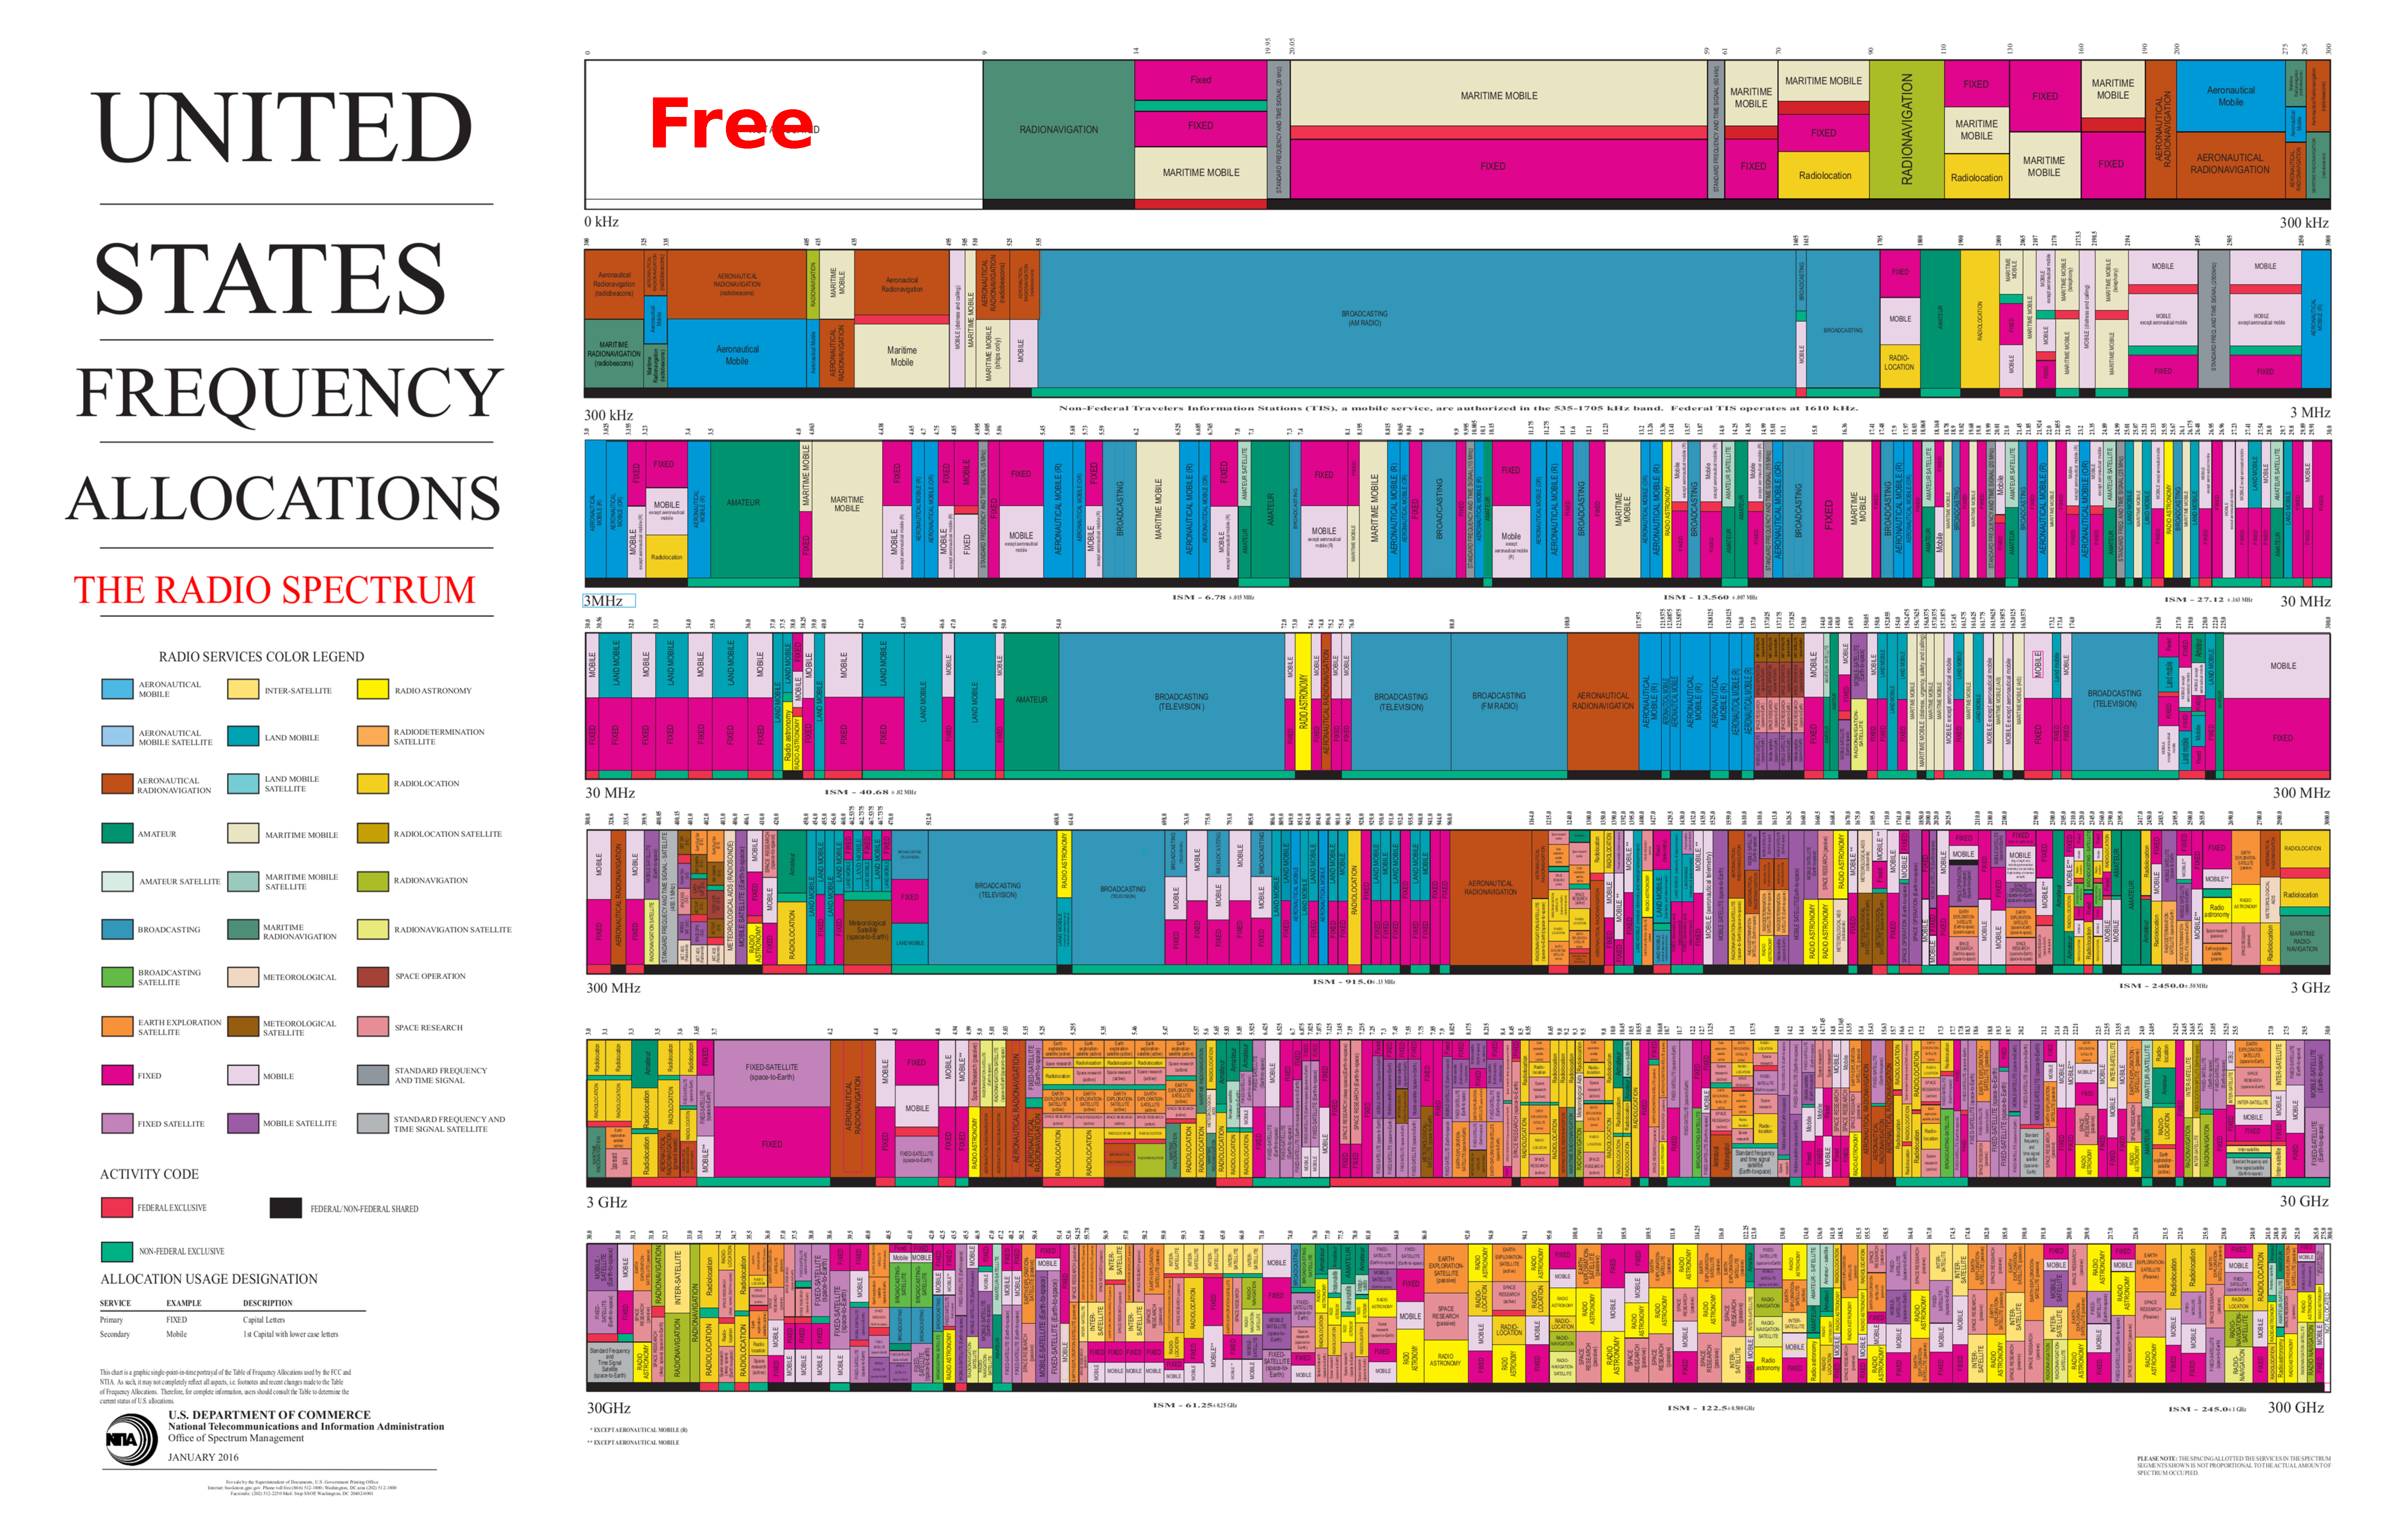
\includegraphics[width=0.65\textwidth]{United_States_Frequency_Allocations_Chart_2016_The_Radio_Spectrum_3}
    \end{center}
    \hfill{}
    {\tiny \textcolor{gray}{United States of North America, Department of Commerce, \textcopyright{} 16}}
\end{frameO}


% \begin{frameO}[But\dots world-wide non-homogeneous frequency usage]
%     But\dots almost everywhere and at anytime in the world, some radio channels are not used! (in any standard)
%     \begin{center}
%         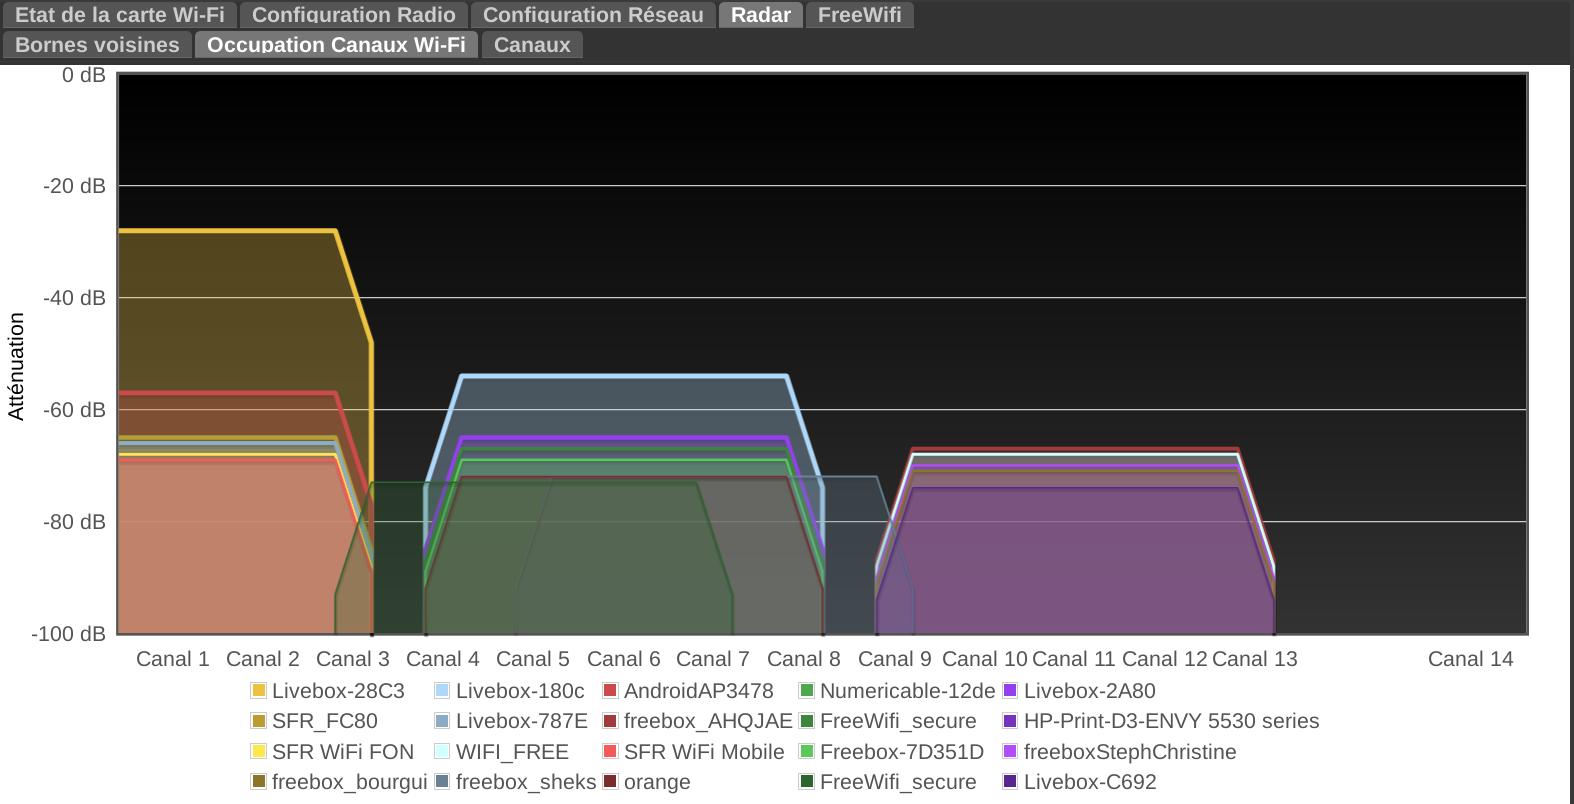
\includegraphics[width=0.80\textwidth]{scan_WiFi_maison}
%     \end{center}
%     \hfill{}
%     {\tiny \textcolor{gray}{Lilian Besson, screenshot from my FreeBox control interface, \textcopyright{} 2019}}

%     \vspace*{10pt}
%     \hfill{}
%     \thinkingface{}
%     \textbf{What if we could dynamically use the (most) empty channels?}
% \end{frameO}


% \begin{frameO}[What did I study during my PhD ? ($1/2$)]
\begin{frameO}[Target of this study]

    % \begin{darkblock}{Telecommunications technology\dots}
    %     \hspace{5pt} $\hookrightarrow$ wireless networks\dots\\
    %     \hspace{10pt} $\hookrightarrow$ networks with decentralized access\dots\\
    %     \hspace{15pt} $\hookrightarrow$ SOME/MANY wireless devices access a wireless network\\
    %     \hspace{30pt} served from ONE access point, in an unlicensed standard:\\
    %     \hspace{30pt} the base station is NOT affecting devices to radio resources\dots\\
    %     \hspace{35pt} $\hookrightarrow$ we focus on the case of \emph{Internet of Things} networks
    % \end{darkblock}

    \begin{darkblock}{Wireless networks\dots}
        % \hspace{5pt} $\hookrightarrow$ \textbf{\alert{wireless} networks}\dots
        \hspace{10pt} $\hookrightarrow$ networks with \textbf{\alert{decentralized} access}\dots

        \hspace{15pt} $\hookrightarrow$ \textbf{\alert{many} wireless devices} 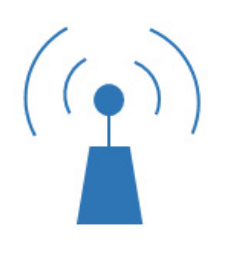
\includegraphics[height=0.37cm]{dynamic-devices.png}  access a wireless network\\
        \hspace{30pt} served from \textbf{\alert{one} access point}\\ % in an unlicensed standard:\\
        \hspace{30pt} the base station is \textbf{\alert{not}} affecting devices to radio resources\dots
    \end{darkblock}

    We focus on \textbf{\alert{Internet of Things}} networks (IoT) in unlicensed bands.

    \pause

    \begin{center}
        % \centering
        
\includegraphics[width=0.50\linewidth]{system_model1.eps}
        % \caption{In our system model, some dynamic devices (in the \textcolor{blue}{IoT network in blue}) transmit packets to a gateway and suffer from the interference generated by neighboring networks (in \textcolor{orange}{orange left/right}).}
        % \label{fig:41:system_model1}
    \end{center}
    % \hfill{}
    % \vspace*{-30pt}
    % {\tiny \textcolor{gray}{[Bonnefoi, Besson et al, CROWNCOM 2017], Ch.5}}

\end{frameO}


\begin{frameO}[The ``Internet of Things'']

    % Test !

    \begin{columns}%[onlytextwidth]
        \begin{column}{0.59\textwidth}
            \begin{colorblock}{Main constraints}
                \small
                \begin{itemize}
                    \item decentralized: \textcolor{orange}{devices initiate transmission}
                    \item can be in unlicensed radio bands
                    \item \textcolor{orange}{massive number of devices}
                    \item long range
                    \item ultra-low power devices
                    \item \textcolor{orange}{low duty cycle}
                    \item \textcolor{orange}{low data rate}
                \end{itemize}
            \end{colorblock}
        \end{column}
        % ...
        \begin{column}{0.40\textwidth}
            % Test !
            \vspace*{10pt}
            % % \begin{center}
                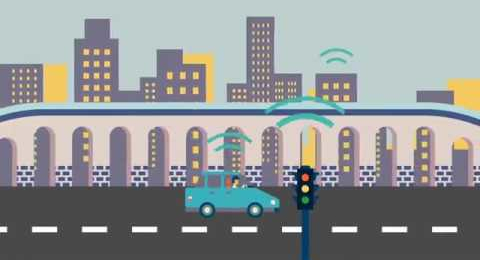
\includegraphics[width=1.00\linewidth]{Screenshot_from_what_is_the_Internet_of_Things_video.jpg}
                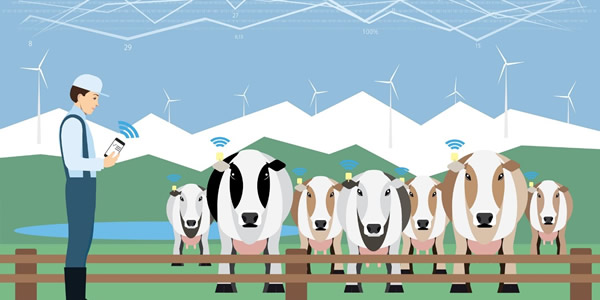
\includegraphics[width=1.00\linewidth]{Connected_cows.jpg}
            % % \end{center}
        \end{column}
    \end{columns}

    \vfill{}
    % \hfill{}
    {\tiny \textcolor{gray}{
        Images from \texttt{http://IBM.com/blogs/internet-of-things/what-is-the-iot}
        % \texttt{YouTu.be/QSIPNhOiMoE} and
        and \texttt{http://www.globalsign.com/en/blog/}\\
        \texttt{connected-cows-and-crop-control}\texttt{-to-drones-the-internet-of-things}\texttt{-is-rapidly-improving-agriculture/}
    }}

\end{frameO}


\begin{frameO}[Main questions]

    \begin{darkblock}{}
        % {Main questions}
        \begin{itemize}
            \item
            Can the IoT devices 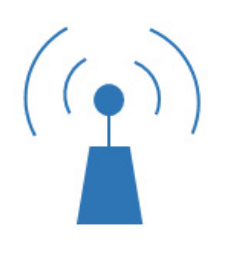
\includegraphics[height=0.37cm]{dynamic-devices.png} optimize their access to the radio resources\\
            in a \textbf{\alert{simple}}, \textbf{\alert{efficient}}, \textbf{\alert{automatic}} and \textbf{\alert{decentralized}} way?\\
            \textcolor{gray}{In a given location, and a given time, for a given radio standard\dots}

            % \item
            % \alert{Can the devices learn \textbf{on their own} to communicate \textbf{more efficiently}?}
        \end{itemize}
    \end{darkblock}

    % \vspace{5pt}
    \pause

    % \begin{colorblock}{Main goals}
        \begin{itemize}
            \item
            Goal: increase the battery life of IoT devices 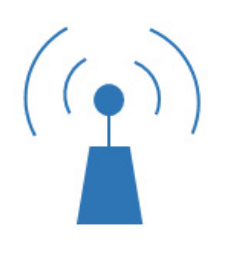
\includegraphics[height=0.37cm]{dynamic-devices.png}
            \item
            Fight the spectrum scarcity issue by using the spectrum more efficiently than a static or uniformly random allocation
        \end{itemize}
    % \end{colorblock}

    % \vspace{5pt}
    \pause

    \begin{lightblock}{\textbf{Main solutions !}}
        % \begin{itemize}
        %     \item
        % Yes we can! By letting the radio devices 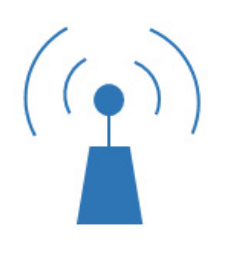
\includegraphics[height=0.37cm]{dynamic-devices.png} become ``intelligent'' \\
        % 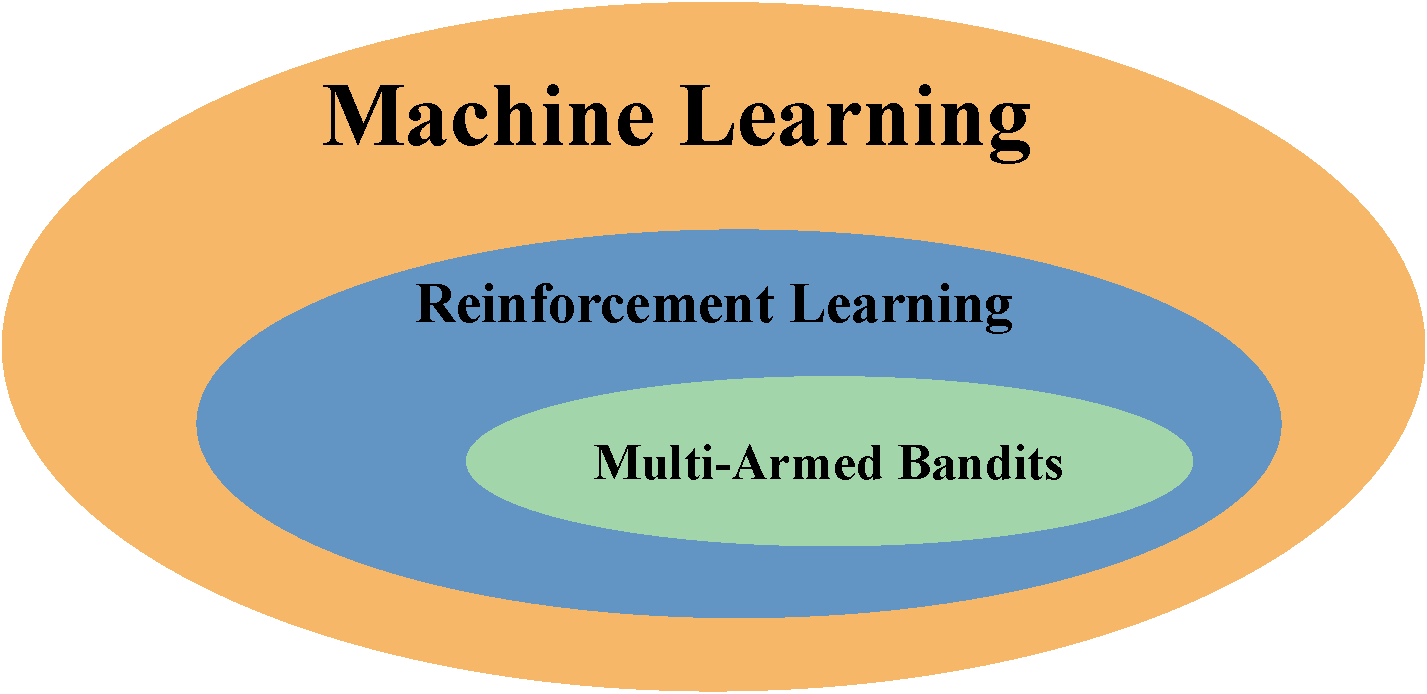
\includegraphics[height=3cm]{Venn_Diagram_ML_RL_MAB.pdf}
        % % \hspace{5pt} $\hookrightarrow$ by using \emph{Machine Learning} algorithms\dots\\
        % % \hspace{10pt} $\hookrightarrow$ of the \emph{Reinforcement Learning} family\dots\\
        % % \hspace{15pt} $\hookrightarrow$ we focus on \textbf{\alert{Multi-Armed Bandit}} algorithms\\
        % % % \hspace{30pt} and we showed they are well suited for (some of) these problems!
        % \end{itemize}

        \begin{columns}%[onlytextwidth]
            \begin{column}{0.50\textwidth}
                \begin{small}
                    \begin{itemize}
                        \item Yes we can! By \textcolor{orange}{letting the radio devices 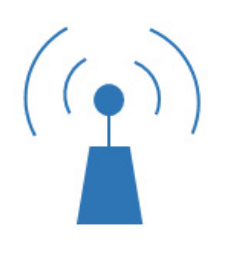
\includegraphics[height=0.37cm]{dynamic-devices.png} become ``intelligent''}
                        \item With \textcolor{darkgreen}{\textbf{MAB algorithms}} !
                    \end{itemize}
                \end{small}
            \end{column}
            % ...
            \begin{column}{0.49\textwidth}
                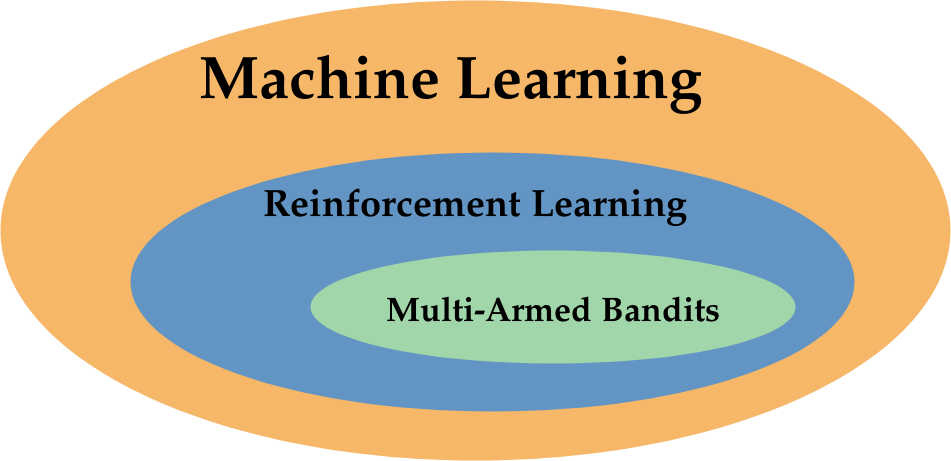
\includegraphics[height=2.75cm]{Venn_Diagram_ML_RL_MAB.png}
                % 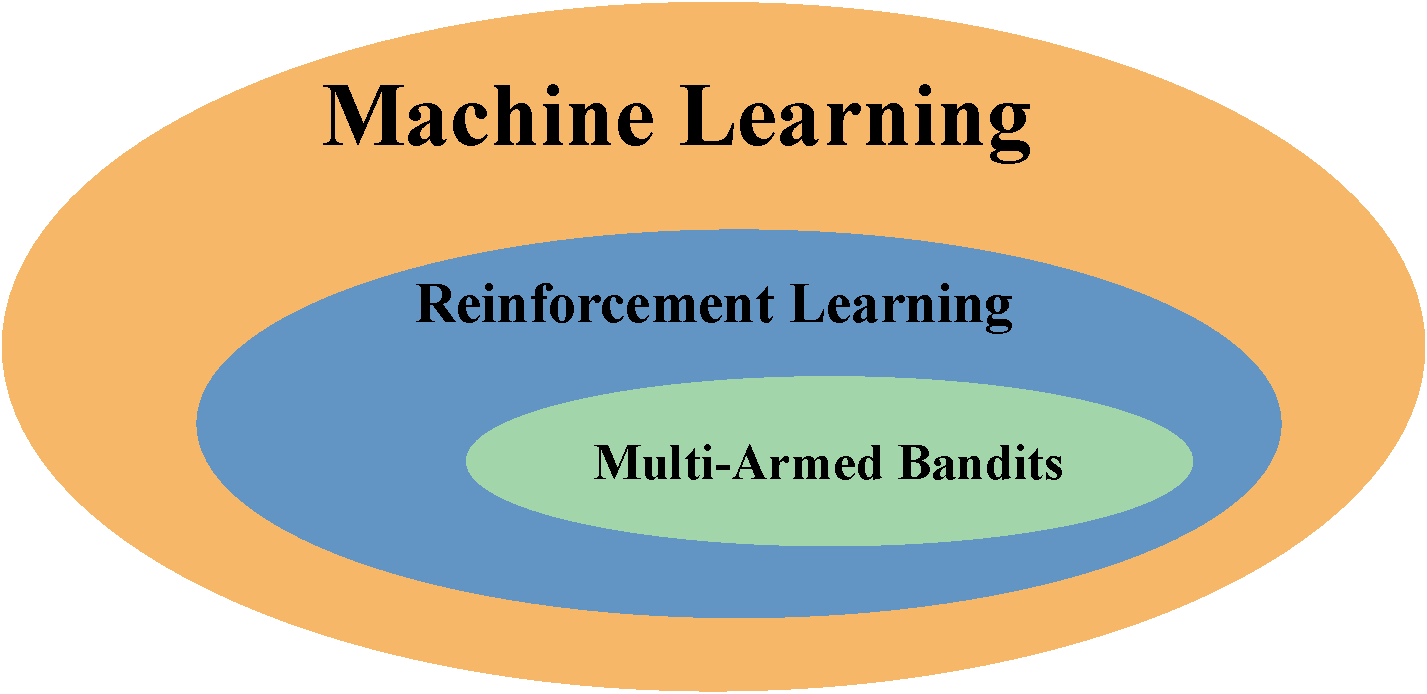
\includegraphics[height=2.75cm]{Venn_Diagram_ML_RL_MAB.pdf}
            \end{column}
        \end{columns}
    \end{lightblock}

\end{frameO}


\section{Outline of this presentation}

\begin{frameTI}
    \color{white}
    \begin{center}
        {\textcolor{white} {\Huge \textsc{Outline of this} }}
    \end{center}
    % \vspace*{5pt}
    \begin{center}
        {\textcolor{white} {\Huge \textsc{presentation} }}
    \end{center}
    % \vspace*{-15pt}
\end{frameTI}


% \begin{frameO}[Main contributions presented today]

%     \large

%     \begin{itemize}
%         \setlength\itemsep{10pt}
%         \item a simple model of IoT network, with decentralized learning embedded in the autonomous IoT devices,
%         \item numerical simulations proving the quality of the proposed solution,
%         \item a realistic implementation on radio hardware,
%         % \item my Python library SMPyBandits.
%         \item theoretical results in a simplified model: multi-player bandits,
%         \item and an extension beyond the stationary hypothesis.
%     \end{itemize}

% \end{frameO}


% \begin{frameO}[Chapters of my thesis addressed today]

%     \large

%     \begin{enumerate}[leftmargin=50pt]
%         \setlength\itemsep{10pt}
%         % \item[Ch.1)] Introduction
%         \item[Ch.2)] \textcolor{blue}{Stochastic Multi-Armed Bandits}
%         \item[\textcolor{gray}{Ch.3)}] \textcolor{gray}{SMPyBandits: an exhaustive Python library to simulate MAB problems}
%         \item[\textcolor{gray}{Ch.4)}] \textcolor{gray}{Expert aggregation for online MAB algorithms selection}
%         \item[Ch.5)] \textcolor{blue}{Improving Spectrum Usage of IoT Networks with Selfish MAB Learning}
%         \item[Ch.6)] \textcolor{blue}{Multi-Players Multi-Armed Bandits}
%         \item[Ch.7)] \textcolor{blue}{Piece-Wise Stationary Bandits}
%         % \item[Ch.8)] General Conclusion and Perspectives
%     \end{enumerate}

% \end{frameO}


% \begin{frameO}[Reading map of my thesis for today]
\begin{frameO}[Contributions of my thesis highlighted today]

    \begin{figure}[h!]
        \centering
        \resizebox{0.95\textwidth}{!}{
        \begin{tikzpicture}[>=latex',line join=bevel,scale=2.25]
            %
            \node[align=center] (introduction) at (0,3.25) [rectangle,draw,fill=blue!15] {\textbf{Chapter~1}\\Introduction};
            \node[align=center] (chapter2) at (0,2.25) [rectangle,draw,fill=green!15] {Chapter~2\\The Stochastic\\Multi-Armed Bandit models};
            \node[align=center] (chapter3) at (-2.5,2.25) [rectangle,draw,fill=gray!10,text=gray] {Chapter~3\\SMPyBandits: simulation\\library for MAB};
            \node[align=center] (chapter25) at (+2.5,2.25) [rectangle,draw,fill=gray!10,text=gray] {Chapter~4\\Online selection\\of the best algorithm};
            \node[align=center] (chapter4) at (-2.5,1) [rectangle,draw,fill=green!25] {\textbf{Chapter~5}\\Two MAB models\\for IoT networks};
            \node[align=center] (chapter5) at (0,1) [rectangle,draw,fill=green!25] {\textbf{Chapter~6}\\Multi-players\\Multi-Armed Bandits};
            \node[align=center] (chapter6) at (2.5,1) [rectangle,draw,fill=green!25] {\textbf{Chapter~7}\\Piece-Wise Stationary\\Multi-Armed Bandits};
            \node[align=center] (conclusion) at (0,-0.25) [rectangle,draw,fill=blue!20] {\textbf{Chapter~8}\\General Conclusion};
            % \node[align=center] (appendix) at (2.5,-0.25) [rectangle,draw,fill=yellow!10] {Appendix};
            %
            \draw [color=black,thick,->] (introduction) to (chapter2);
            \draw [color=black,dotted,->] (chapter2) to (chapter3);
            \draw [color=black,dotted,->] (chapter2) to (chapter25);
            \draw [color=black,thick,->] (chapter2) to (chapter4);
            % \draw [color=black,thick,->] (chapter2) to (chapter5);
            \draw [color=black,thick,->]   (chapter4) to (chapter5);
            % \draw [color=black,densely dotted,->] -| (chapter3) to (chapter25);
            % \draw [color=black,densely dotted,->] -| (chapter25) to (chapter6);
            \draw [color=black,thick,->]   (chapter5) to (chapter6);
            % \draw [color=black,thick,->] (chapter2) to (chapter6);
            % \draw [color=black,thick,->] (chapter4) to (conclusion);
            % \draw [color=black,thick,->] (chapter5) to (conclusion);
            \draw [color=black,thick,->] (chapter6) to (conclusion);
            % \draw [color=black,thick,->] (conclusion) to (appendix);
            %
        \end{tikzpicture}
        }
        % \caption[Organization of the thesis: a reading map.]{A reading map of the thesis. Any top-down path containing Chapter~\ref{chapter:1}, Chapter~\ref{chapter:2}, at least one of the three Chapters~\ref{chapter:4}, \ref{chapter:5} and \ref{chapter:6}, and the Conclusion is a self contained way to read this thesis.}
        \label{fig:1:organization}
    \end{figure}
\end{frameO}


\begin{frameO}[Outline of this presentation]
    \begin{large}

    \begin{itemize}
        \setlength\itemsep{2em}
        \item \textcolor{gray}{\textbf{Introduction.} Spectrum issues in wireless networks}
        % \item \textcolor{gray}{\sout{The Stochastic Multi-Armed Bandit models}}
        % \begin{itemize}
        %     \item \textcolor{gray}{applying bandit to Opportunistic Spectrum Access (OSA)}
        %     \item \textcolor{gray}{performance measure (regret) and first strategies}
        %     \item \textcolor{gray}{best possible regret? Lower bounds}
        %     \item \textcolor{gray}{upper Confidence Bounds (UCB) Algorithms}
        % \end{itemize}
        \item \textbf{Part I.} Selfish MAB learning in a new model of IoT network
        % \begin{itemize}
        %     % \item \textcolor{gray}{reference strategies}
        %     \item \textcolor{gray}{selfish applications of MAB algorithms}
        %     \item \textcolor{gray}{numerical simulations and illustrations}
        %     \item \textcolor{gray}{realistic implementation on real radio hardware}
        %     \item \textcolor{gray}{\emph{intractable} model in theory\dots}
        % \end{itemize}
        \item \textbf{Part II.} \emph{Two tractable problems} extending the classical bandit
        \begin{itemize}
            \item \textcolor{gray}{multi-player bandits in stationary settings}
            \item \textcolor{gray}{single-player bandits in piece-wise stationary settings}
        \end{itemize}
        \item \textbf{Conclusion and perspectives}
    \end{itemize}

    \end{large}

\end{frameO}



% \section{Introduction to Multi-Armed Bandits}

% \begin{frameTI}
%     \begin{center}
%         {\textcolor{white} {\Huge \textsc{Introduction to Multi-Armed Bandits} }}
%     \end{center}
%     \vspace*{-4pt}
% \end{frameTI}

% \begin{frame}[c]
%     \begin{changemargin}{-0.5cm}{-0.5cm}
%         \begin{center}
%             \vspace{-0.3in}
%             \textbf{\huge Introduction to Multi-Armed Bandits}
%             \vspace{1.5cm}

%             \textbf{\Large Why Bandits?}\\[0.5cm]
%             \textcolor{darkgray}{\textbf{\Large Performance measure}\\[0.5cm] }
%             \textcolor{darkgray}{\textbf{\Large Best possible regret?}\\[0.5cm] }
%             \textcolor{darkgray}{\textbf{\Large The optimism principle}\\[0.5cm] }
%         \end{center}
%     \end{changemargin}
% \end{frame}



% \begin{frameO}[Hum, what is a \emph{bandit}?]
%     \begin{center}
%         It's an old name for a casino machine!
%     \end{center}

%     \begin{center}
%         
\includegraphics[height=7cm]{Lucky_Luke__Le_Bandit_Manchot.jpg}

%         \begin{tiny}
%             \textcolor{gray}{
%                 \textcopyright{} Dargaud,
%                 \href{https://www.dargaud.com/bd/LUCKY-LUKE/Lucky-Luke/Lucky-Luke-tome-18-Bandit-manchot-Le}{\textcolor{blue}{Lucky Luke tome 18}}.
%             }
%         \end{tiny}
%     \end{center}
% \end{frameO}


% \begin{frameO}[Make money in a casino?]
%     \begin{center}
%         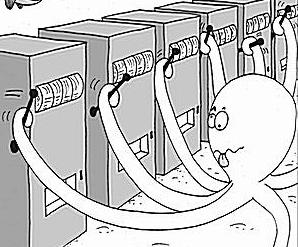
\includegraphics[height=3cm]{MABpieuvre}
%     \end{center}
%     \begin{center}
%         A (single) \blue agent \black facing (multiple) \red arms \black in a Multi-Armed Bandit.
%     \end{center}

%     \pause
%     \begin{center}
%         \Huge NO!
%     \end{center}
% \end{frameO}

% \begin{frameO}[Sequential resource allocation]
%     \textbf{Clinical trials}
%     \begin{itemize}
%         \item $K$ treatments for a given symptom (with unknown effect)

%               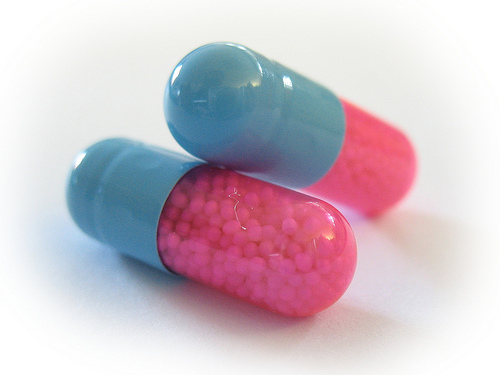
\includegraphics[width=0.12\linewidth]{medoc1.jpg}
%               \hspace{0.05cm}
%               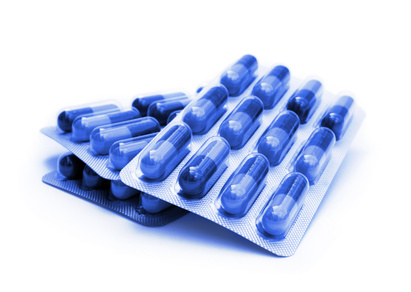
\includegraphics[width=0.12\linewidth]{medoc4.jpg}
%               \hspace{0.05cm}
%               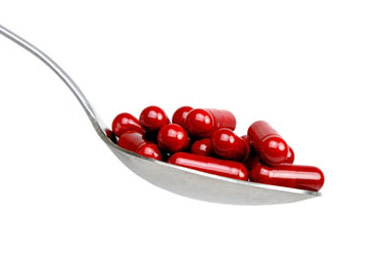
\includegraphics[width=0.12\linewidth]{medoc3.jpg}
%               \hspace{0.05cm}
%               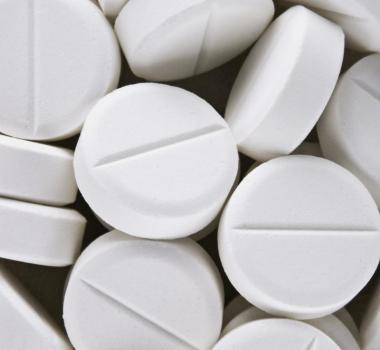
\includegraphics[width=0.12\linewidth]{medoc2.jpg}
%               \hspace{0.05cm}
%               
\includegraphics[width=0.12\linewidth]{medoc5.jpg}
%               \hspace{0.05cm}
%               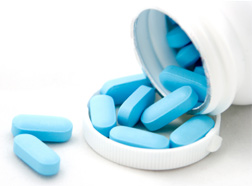
\includegraphics[width=0.12\linewidth]{medoc6.jpg}
%               \hspace{0.05cm}

%         \item What treatment should be allocated to the next patient, based on responses observed on previous patients?
%     \end{itemize}

%     \vspace{0.2cm}

%     \pause

%     \textbf{Online advertisement}
%     \begin{itemize}
%         \item $K$ adds that can be displayed
%               \vspace{0.1cm}

%               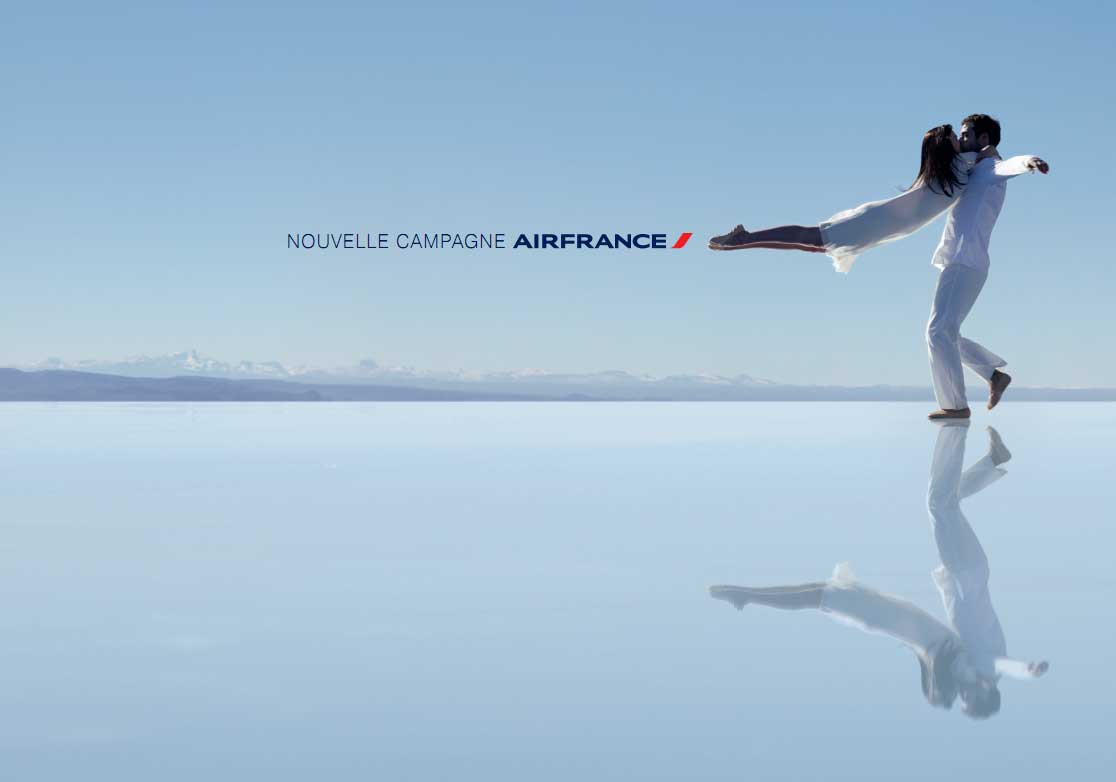
\includegraphics[height=0.15\paperheight]{ad6.jpg}
%               \hspace{0.1cm}
%               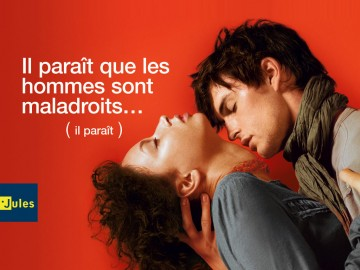
\includegraphics[height=0.15\paperheight]{ad2.jpg}
%               \hspace{0.1cm}
%               
\includegraphics[height=0.15\paperheight]{ad4.jpg}
%               \hspace{0.1cm}
%               
\includegraphics[height=0.15\paperheight]{ad5.jpg}
%               \hspace{0.05cm}

%         \item Which add should be displayed for a user, based on the previous clicks of previous (similar) users?
%     \end{itemize}

% \end{frameO}



% % \begin{frameO}[Dynamic allocation of computational resources]

% %     \vspace{0.4cm}

% %     \textbf{Numerical experiments} (bandits for ``black-box'' optimization)

% %     \vspace{-0.3cm}

% %     \begin{center}
% %         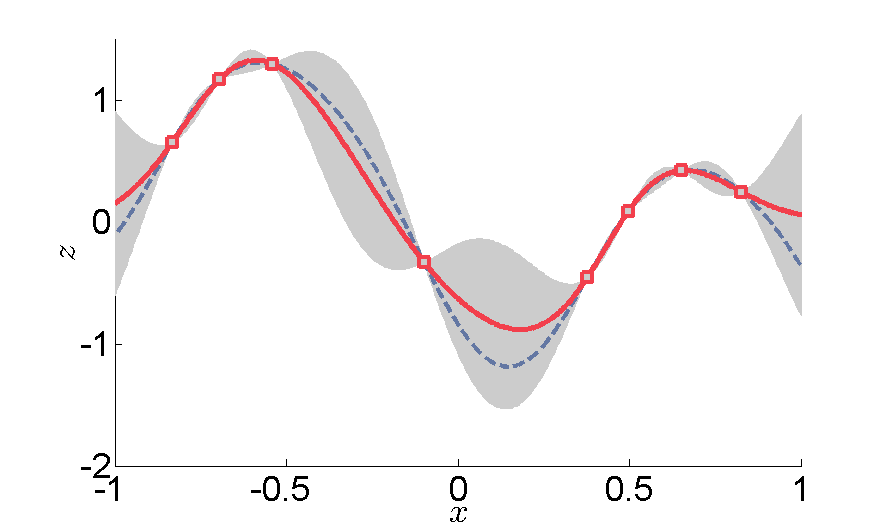
\includegraphics[height=2.5cm]{GP}
% %     \end{center}

% %     \vspace{-0.3cm}

% %     \begin{itemize}
% %         \item where to evaluate a costly function in order to find its maximum?
% %     \end{itemize}

% %     \pause

% %     \textbf{Artificial intelligence for games}

% %     \begin{center}
% %         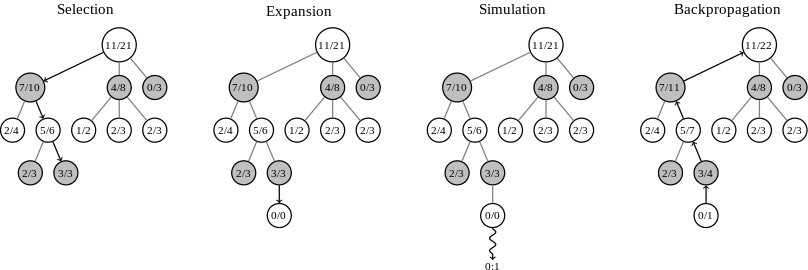
\includegraphics[height=2.2cm]{MCTSWiki}
% %     \end{center}

% %     \vspace{-0.5cm}

% %     \begin{itemize}
% %         \item where to choose the next evaluation to perform in order to find the best move to play next?
% %     \end{itemize}

% % \end{frameO}


% \begin{frameO}[Dynamic channel selection]

%     \vspace{0.3cm}

%     \textbf{Communications in presence of a central controller}
%     \begin{itemize}
%         \item $K$ assignments from $n$ users to $m$ antennas ($\rightsquigarrow$ \emph{combinatorial} bandit)

%               \hspace{2.5cm}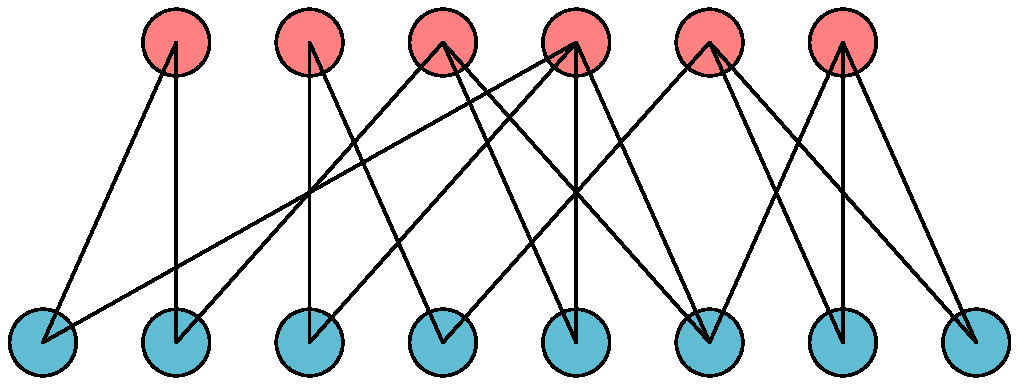
\includegraphics[height=0.2\paperheight]{assignements}
%         \item How to select the next \emph{matching} based on the throughput observed in previous communications?
%     \end{itemize}

%     \vspace{0.1cm}

%     \pause

%     \textbf{Opportunistic Spectrum Access (OSA)}
%     \begin{itemize}
%         \item $K$ radio channels (orthogonal frequency bands)

%               \hspace{0.4cm}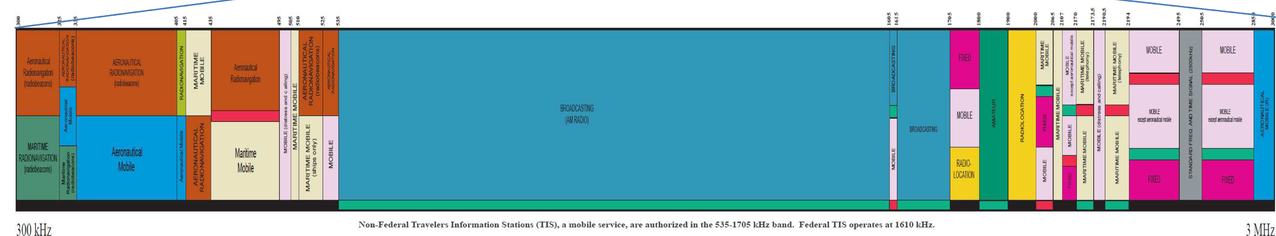
\includegraphics[height=0.17\paperheight]{spectrum}
%         \item In which channel should a radio device send a packet, based on the quality of its previous communications?
%     \end{itemize}

% \end{frameO}


% %%% TITLE SLIDE FOR PART I


% % standard slides for Part I

% \setbeamertemplate{background canvas}{
\includegraphics[width=\paperwidth,height=\paperheight]{../templateCS/PageTabInverse_CentraleSupelec}}

% \setbeamertemplate{footline}{\hspace{2cm} \raisebox{2.5ex}
%     {\textcolor{white}{PhD defense -- Lilian Besson -- \emph{``MAB Algorithms for IoT Networks''}}}\hfill
%     \raisebox{2.5ex}
%     {\textcolor{white}{20 November, 2019 -- \insertframenumber / \inserttotalframenumber \hspace{5mm} \null }}}

% \subsection{Multi-armed Bandit}

% \begin{frameO}[\alt<2>{The \blue Stochastic \color{white} Multi-Armed Bandit Setup}{The Multi-Armed Bandit Setup}]

%     \alt<2>{\vspace{0.4cm}}{}

%     \begin{center}
%         $K$ \textbf{arms} $\Leftrightarrow$ $K$ \alt<2>{\blue probability distributions \black : $\nu_a$ has mean $\blue\mu_a$}{rewards streams $(X_{a,t})_{t\in\N}$}
%     \end{center}

%     \begin{center}
%         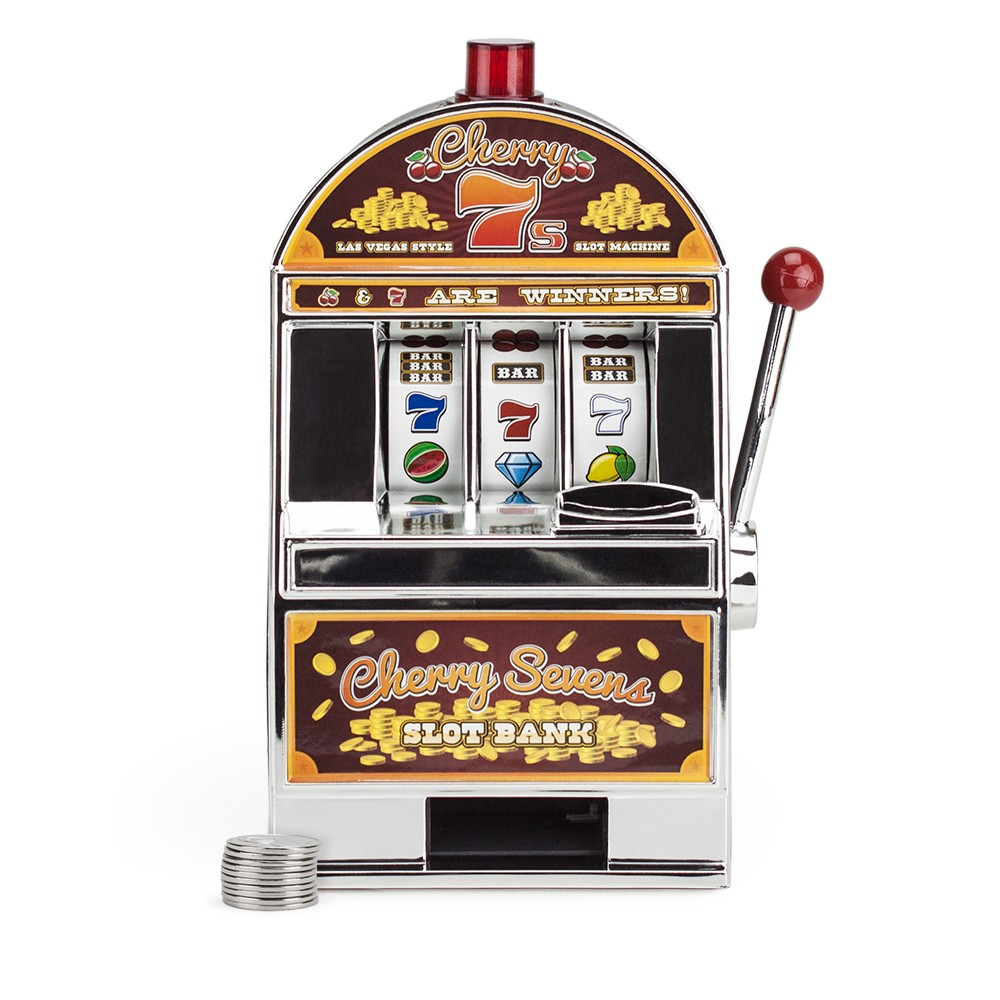
\includegraphics[height=0.15\textheight]{slot1.jpg}
%         \hspace{0.4cm}
%         \includegraphics[height=0.15\textheight]{slot2.jpg}
%         \hspace{0.4cm}
%         \includegraphics[height=0.15\textheight]{slot3.jpg}
%         \hspace{0.4cm}
%         \includegraphics[height=0.15\textheight]{slot4.jpg}
%         \hspace{0.5cm}
%         \includegraphics[height=0.15\textheight]{slot5.jpg}
%         \hspace{0.4cm}
%     \end{center}

%     \vspace{-0.8cm}

%     \[ \alt<2>{\blue\nu_1}{} \hspace{1.4cm} \alt<2>{\blue\nu_2}{} \hspace{1.4cm} \alt<2>{\blue\nu_3}{} \hspace{1.4cm} \alt<2>{\blue\nu_4}{} \hspace{1.4cm} \alt<2>{\blue\nu_5}{}\]

%     \alt<2>{\vspace{-0.4cm}}{}

%     At round $t$, an agent:
%     \begin{itemize}
%         \item chooses an  arm $A_t$
%         \item receives a reward \alt<2>{$R_t = X_{A_t,t}\blue \overset{\text{iid}}{\sim} \nu_{A_t}$ (i.i.d. from a distribution)}{$R_t = X_{A_t,t}$ (from the environment)}
%     \end{itemize}

%     \vspace{0.2cm}

%     \red Sequential \black sampling strategy (\textbf{bandit algorithm}):
%     $\red A_{t+1} = F_t (A_1,R_1,\dots,A_{t},R_{t})\black$.

%     \textbf{Goal:} Maximize sum of rewards \alt<2>{$\blue \bE\black\left[\sum\limits_{t=1}^T R_t\right]$}{$\sum\limits_{t=1}^T R_t$}.


% \end{frameO}

% \begin{frameO}[Discover bandits by playing this online demo!]

%     \begin{center}
%         \includegraphics[width=0.75\textwidth]{example_of_a_5_arm_bandit_problem.png}
%     \end{center}

%     % \begin{small}
%     $\hookrightarrow$ Interactive demo on this web-page
%     \href{https://perso.crans.org/besson/phd/MAB_interactive_demo/}{\textcolor{blue}{\texttt{perso.crans.org/besson/phd/MAB\_interactive\_demo/}}}
%     % Ref: [Bandits Algorithms, Lattimore \& Szepesv{\'a}ri, 2019],
%     % on \href{https://tor-lattimore.com/downloads/book/book.pdf}{\textcolor{blue}{\texttt{tor-lattimore.com/downloads/book/book.pdf}}}
%     % \end{small}

% \end{frameO}

% % \begin{frameO}[Clinical trials]

% %     \textbf{Historical motivation} \color{gray}[Thompson 1933]\color{black}

% %     \begin{center}
% %         \includegraphics[width=0.12\linewidth]{medoc1.jpg}
% %         \hspace{0.3cm}
% %         \includegraphics[width=0.12\linewidth]{medoc4.jpg}
% %         \hspace{0.3cm}
% %         \includegraphics[width=0.12\linewidth]{medoc3.jpg}
% %         \hspace{0.5cm}
% %         \includegraphics[width=0.12\linewidth]{medoc2.jpg}
% %         \hspace{0.5cm}
% %         \includegraphics[width=0.12\linewidth]{medoc5.jpg}
% %         \hspace{0.3cm}
% %     \end{center}
% %     \vspace{-0.8cm}

% %     \hspace{-0.3cm}\[ \cB(\mu_1) \hspace{0.9cm} \cB(\mu_2) \hspace{0.9cm} \cB(\mu_3) \hspace{0.8cm} \cB(\mu_4) \hspace{0.9cm} \cB(\mu_5)\]

% %     For the $t$-th patient in a clinical study,

% %     \begin{itemize}
% %         \item chooses a \blue treatment $A_t$\black
% %         \item observes a (Bernoulli) \blue response $R_t \in \{0,1\} : \bP(R_t = 1 | A_t = a) = \mu_{a}$\black
% %     \end{itemize}

% %     \vspace{0.3cm}


% %     \textbf{Goal:} maximize the expected number of patients healed.

% % \end{frameO}



% % \begin{frameO}[Online content optimization]

% %     \textbf{Modern motivation} ($\$\$\$\$$) \gray [Li et al, 2010] \black

% %     (recommender systems, online advertisement, etc)


% %     \begin{center}
% %         \includegraphics[height=0.15\textheight]{film1.jpg}
% %         \hspace{0.6cm}
% %         \includegraphics[height=0.15\textheight]{film2.jpg}
% %         \hspace{0.6cm}
% %         \includegraphics[height=0.15\textheight]{film3.jpg}
% %         \hspace{0.6cm}
% %         \includegraphics[height=0.15\textheight]{film4.jpg}
% %         \hspace{0.6cm}
% %         \includegraphics[height=0.15\textheight]{film5.jpg}
% %         \hspace{0.6cm}
% %     \end{center}

% %     \vspace{-0.8cm}

% %     \hspace{-0.2cm}\[ \nu_1 \hspace{1.4cm} \nu_2 \hspace{1.4cm} \nu_3 \hspace{1.4cm} \nu_4 \hspace{1.4cm} \nu_5\]

% %     For the $t$-th visitor of a website,
% %     \begin{itemize}
% %         \item recommend a  \blue movie $A_t$\black
% %         \item observe a \blue rating $R_t \sim \nu_{A_t}$\black \ (e.g. $R_t \in \{1,\dots,5\}$)
% %     \end{itemize}

% %     \vspace{0.3cm}

% %     \textbf{Goal:} maximize the sum of ratings.

% % \end{frameO}


% \begin{frameO}[Application to Cognitive Radios: OSA]

%     \textbf{Opportunistic Spectrum Access}
%     \textcolor{gray}{
%         % [Liu \& Zhao, 2010]
%         % [Anandkumar et al. 2011]
%         [Jouini, Moy et al. 2010]
%     }

%     \begin{center}

%         \emph{streams indicating channel quality}

%         \vspace{0.3cm}

%         \begin{tabular}{|c||c|c|c|c|c|c|c|}
%             \hline
%             Channel $1$ & \cellcolor{blue!25}$X_{1,1}$ & $X_{1,2}$                    & \dots & $X_{1,t}$                    & \dots & $X_{1,T}$                    & $\sim \nu_1$ \\
%             \hline
%             Channel $2$ & $X_{2,1}$                    & \cellcolor{blue!25}$X_{2,2}$ & \dots & $X_{2,t}$                    & \dots & \cellcolor{blue!25}$X_{2,T}$ & $\sim \nu_2$ \\
%             \hline
%             \dots       & \dots                        & \dots                        & \dots & \dots                        & \dots & \dots                        & \dots        \\
%             \hline
%             Channel $K$ & $X_{K,1}$                    & $X_{K,2}$                    & \dots & \cellcolor{blue!25}$X_{K,t}$ & \dots & $X_{K,T}$                    & $\sim \nu_K$ \\
%             \hline
%         \end{tabular}
%     \end{center}

%     \vspace{0.2cm}

%     At round $t$, the device:
%     \begin{itemize}
%         \item selects \blue{a channel} $A_t \in \{1,\dots,K\}$\black
%         \item observes the \blue quality of its communication  $R_t = X_{A_t,t} \in [0,1]$\black
%         \begin{itemize}
%             \item $R_T \in\{0,1\}$ binary reward: success/failure of message transmission
%             \item $R_T \in[0,1]$ continuous reward: e.g., received power,  etc
%         \end{itemize}
%     \end{itemize}

%     \vspace{0.2cm}

%     \textbf{Goal:} Maximize the overall quality of communications.

% \end{frameO}



% \subsection{Performance measure and first strategies}

% \begin{frame}[c]
%     \begin{changemargin}{-0.5cm}{-0.5cm}
%         \begin{center}
%             \vspace{-0.3in}
%             \textbf{\huge Introduction to Multi-Armed Bandits}
%             \vspace{1.5cm}

%             \textcolor{darkgray}{\textbf{\Large Why Bandits?}\\[0.5cm]}
%             \textbf{\Large Performance measure and first strategies}\\[0.5cm]
%             \textcolor{darkgray}{\textbf{\Large Best possible regret?}\\[0.5cm] }
%             \textcolor{darkgray}{\textbf{\Large The optimism principle}\\[0.5cm] }
%         \end{center}
%     \end{changemargin}
% \end{frame}


% \begin{frameO}[Regret of a bandit algorithm]

%     \bigskip

%     \textbf{Bandit instance:} $\bm\nu = (\nu_1,\nu_2, \dots,\nu_K)$, mean of arm $a$: $\mu_a = \bE_{X \sim \nu_a}[X]$.

%     \[\red\mu_\star = \max_{a \in \{1,\dots,K\}} \mu_a \ \ \text{and} \ \ \ a_\star = \argmax_{a \in \{1,\dots,K\}} \mu_a.\]
%     \[\begin{array}{ccl}\text{Maximizing rewards} & \Leftrightarrow & \text{selecting } a_\star \text{ as much as possible }         \\
%                                            & \Leftrightarrow & \text{minimizing the \blue regret } \gray \text{[Robbins, 52]}
%         \end{array}\]

%     \vspace{-0.4cm}

%     \begin{eqnarray*}
%         \blue \cR_{\bm\nu}(\cA,T) \eqdef \black\underbrace{\blue T \mu_\star}_{\substack{\text{sum of rewards of}\\ \text{an oracle strategy} \\ \text{always selecting } a_\star}} \blue- \black\underbrace{\blue\bE\left[\sum_{t=1}^{T}R_{t}\right]}_{\substack{\text{sum of rewards of}\\\text{the strategy} \cA}}
%     \end{eqnarray*}

%     \vspace{-0.4cm}
%     \pause

%     \begin{colorblock}{What regret rate can we achieve?}
%         \begin{itemize}
%             \item[$\Longrightarrow$] consistency \black $\cR_{\bm\nu}(\cA,T) / T \Longrightarrow 0$ (when $T\to\infty$)
%             \item[$\Longrightarrow$] can we be more precise?
%         \end{itemize}
%     \end{colorblock}
% \end{frameO}

% \begin{frameO}[Regret decomposition]

%     \vspace{0.6cm}

%     $N_a(t)$ : number of selections of arm $a$ in the first $t$ rounds

%     $\Delta_a \eqdef \mu_\star -\mu_a$ : sub-optimality gap of arm $a$

%     \begin{colorblock}{Regret decomposition}
%         \[\alert<1>{ \cR_{\bm\nu}(\cA,T) = \sum_{a=1}^K \Delta_a \bE\left[N_a(T)\right] }.\]
%     \end{colorblock}
%     \pause

%     \vspace{0.6cm}

%     A strategy with small regret should:
%     \begin{itemize}
%         \item select not too often arms for which $\Delta_a > 0$ (sub-optimal arms)
%         \item \dots which requires to try all arms to estimate the values of the $\Delta_a$
%     \end{itemize}

%     \vspace{0.5cm}

%     \begin{center}
%         \red $\Longrightarrow$ Exploration / Exploitation trade-off !
%     \end{center}

% \end{frameO}


% \begin{frameO}[Two naive strategies]

%     \vspace{0.4cm}

%     \begin{itemize}
%         \item \textbf{Idea 1 :}
%               \hfill{} \color{red}$\Longrightarrow$ EXPLORATION \color{black}
%               \begin{colorblock}{}Draw each arm $T/K$ times\end{colorblock}
%     \end{itemize}

%     \vspace{-0.3cm}

%     \[\hookrightarrow \cR_{\bm\nu}(\cA,T) = \left(\frac{1}{K}\sum_{a : \mu_a > \mu_\star} \Delta_a\right) T = \alert{\Omega(T)} \]

%     \pause

%     \begin{itemize}
%         \item \textbf{Idea 2 :} Always trust the empirical best arm
%               \hfill{} \color{red}$\Longrightarrow$ EXPLOITATION \color{black}
%     \end{itemize}
%     \begin{colorblock}{}
%         $A_{t+1}=\underset{a \in \{1,\dots,K\}}{\text{argmax}} \ \blue \widehat{\mu}_a(t)$
%         using estimates of the unknown means $\mu_a$

%         \[\blue \widehat{\mu}_a(t) =\frac{1}{N_a(t)}\sum_{s=1}^t X_{a,s} \ind_{(A_s=a)}\]
%     \end{colorblock}

%     \vspace{-0.3cm}

%     \[\hspace{1.5cm} \hookrightarrow \cR_{\bm\nu}(\cA,T) \geq  (1-\mu_1)\times \mu_2 \times (\mu_1 - \mu_2) T  = \alert{\Omega(T)} \]
%     \begin{center}\vspace{-0.2cm}
%         \hspace{1.5cm}(with $K=2$ Bernoulli arms of means $\mu_1 \neq \mu_2$)
%     \end{center}


% \end{frameO}



% \subsection{Best possible regret? Lower bounds}

% \begin{frame}[c]
%     \begin{changemargin}{-0.5cm}{-0.5cm}
%         \begin{center}
%             \vspace{-0.3in}
%             \textbf{\huge Introduction to Multi-Armed Bandits}
%             \vspace{1.5cm}

%             \textcolor{darkgray}{\textbf{\Large Why Bandits?}\\[0.5cm]}
%             \textcolor{darkgray}{\textbf{\Large Performance measure and first strategies}\\[0.5cm]}
%             \textbf{\Large Best possible regret? Lower bounds}\\[0.5cm]
%             \textcolor{darkgray}{\textbf{\Large The optimism principle}\\[0.5cm] }
%         \end{center}
%     \end{changemargin}
% \end{frame}


% \begin{frameO}[The Lai and Robbins lower bound]

%     \vspace{0.3cm}

%     \textbf{Context:} a \blue parametric bandit model \black where each arm is parameterized by its mean $\bm\nu =(\nu_{\mu_1},\dots,\nu_{\mu_K})$, $\mu_a \in \cI$.
%     \[ \text{distributions } \bm\nu \ \ \Leftrightarrow \ \ \bm\mu = (\mu_1,\dots,\mu_K) \text{ means} \]


%     \textbf{Key tool:} \blue Kullback-Leibler divergence\black.

%     \begin{colorblock}{Kullback-Leibler divergence}

%         \alt<3>{\vspace{-0.2cm}}{}

%         \[
%             \red \mathrm{kl}(\mu,\mu')  \black : =   \alt<3>{\mu\log \left(\frac{\mu}{\mu'}\right) + (1-\mu) \log \left(\frac{1-\mu}{1-\mu'}\right) \ \ \ (\text{Bernoulli bandits})}{\alt<2>{\frac{(\mu - \mu')^2}{2\sigma^2} \ \ \ (\text{Gaussian bandits with variance } \sigma^2)}{\text{KL}\left(\nu_\mu,\nu_{\mu'}\right) =\bE_{X \sim \nu_{\mu}}\left[\log \frac{d\nu_{\mu}}{d\nu_{\mu'}}(X)\right]}}
%         \]


%         \vspace{-0.3cm}

%     \end{colorblock}
%     \begin{colorblock}{Theorem \hfill{} \textcolor{gray}{[Lai and Robbins, 1985]}}
%         For uniformly efficient algorithms ($\cR_{\bm\mu}(\cA,T)=o(T^\alpha)$ for all $\alpha\in (0,1)$ and $\bm \mu \in \cI^K$),

%         \vspace{-0.4cm}

%         \[
%             \color{red}\mu_a<\mu_\star \Longrightarrow \liminf_{T\rightarrow\infty}\frac{\bE_{\bm \mu}[N_{a}(T)]}{\log T}\geq \frac{1}{\mathrm{kl}(\mu_a,\mu_\star)}.\color{black}
%         \]

%         \vspace{-0.3cm}

%     \end{colorblock}

% \end{frameO}


% \begin{frameO}[Other asymptotic lower bounds]

%     Such asymptotic lower bound can be generalized to extensions of the stationary single-player MAB model
%     $ \cR(\cA, T) \geq \Omega(C_{\text{problem}} K \log(T)) $.

%     \vspace*{2pt}

%     \begin{lightblock}{For \textbf{multi-player bandits} \hfill{} (with $2 \leq M \leq K$ players)}
%         Same lower-bound, with a problem-dependent constant $C'_{\text{problem}}$
%         \[ \cR(\cA, T) \geq \Omega(C'_{\text{problem}} M K \log(T)). \]
%     \end{lightblock}

%     \vspace*{2pt}

%     \begin{lightblock}{For \textbf{piece-wise stationary bandits} \hfill{} (with $\Upsilon_T$ stationary intervals)}
%         Larger lower-bound, with a problem-dependent constant $C''_{\text{problem}}$
%         \[ \cR(\cA, T) \geq \Omega(C''_{\text{problem}} \sqrt{K \Upsilon_T T}). \]
%     \end{lightblock}

%     \textcolor{gray}{(our proposed algorithms are asymptotically matching the lower-bounds)}

% \end{frameO}



% \subsection{The Optimism Principle and Upper Confidence Bounds Algorithms}

% \begin{frame}[c]
%     \begin{changemargin}{-0.5cm}{-0.5cm}
%         \begin{center}
%             \vspace{-0.3in}
%             \textbf{\huge Introduction to Multi-Armed Bandits}
%             \vspace{1.5cm}

%             \textcolor{darkgray}{\textbf{\Large Why Bandits?}\\[0.5cm]}
%             \textcolor{darkgray}{\textbf{\Large Performance measure and first strategies}\\[0.5cm]}
%             \textcolor{darkgray}{\textbf{\Large Best possible regret? Lower bounds}\\[0.5cm]}
%             \textbf{\Large The optimism principle:\\
%                 Upper Confidence Bounds Algorithms}\\[0.5cm]
%         \end{center}
%     \end{changemargin}
% \end{frame}


% \begin{frameO}[A first UCB algorithm]

%     \vspace{0.3cm}

%     \begin{itemize}
%         \item $N_a(t) = \sum_{s=1}^t\ind_{(A_s = a)}$ number of selections of $a$ after $t$ rounds
%         \item $\hat \mu_{a,s} = \frac{1}{s}\sum_{k=1}^s Y_{a,k}$ average of the first $s$ observations from arm $a$
%         \item $\widehat{\mu}_a(t) = \widehat{\mu}_{a,N_a(t)}$ empirical estimate of $\mu_a$ after $t$ rounds
%     \end{itemize}

%     \vspace{0.3cm}

%     UCB($\alpha$) selects  $A_{t+1} = \argmax_a \ \mathrm{UCB}_a(t)$
%     where
%     \[\blue \mathrm{UCB}_a(t) =\black \underbrace{\blue \widehat{\mu}_{a}(t)}_{\text{exploitation term}} + \underbrace{\blue\sqrt{\frac{\alpha\log(t)}{N_a(t)}}}_{\text{exploration bonus}}.\]

%     \vspace{0.3cm}

%     \begin{colorblock}{Hoeffding inequality + union bound \hfill{} \textcolor{gray}{[Auer et al. 2002]}}
%         \[ \bP\left(\mu_a \leq \red \widehat{\mu}_a(t) + \sigma\sqrt{\frac{\alpha\log(t)}{N_a(t)}} \black \right) \geq 1 - \frac{1}{t^{\frac{\alpha}{2} -1}} \]
%     \end{colorblock}

%     % \pause
%     % \textbf{Proof.}

%     % \vspace{-0.5cm}

%     % \begin{align*}
%     %      & \bP\left(\mu_a > \widehat{\mu}_a(t) + \sigma\sqrt{\frac{\alpha\log(t)}{N_a(t)}} \black \right) \leq  \bP\left(\exists s \leq t : \mu_a > \widehat{\mu}_{a,s} + \sigma\sqrt{\frac{\alpha\log(t)}{s}} \black\right) \\
%     %      & \leq \sum_{s=1}^t \bP\left(\widehat{\mu}_{a,s} < \mu_a - \sigma\sqrt{\frac{\alpha\log(t)}{s}}\right) \leq \sum_{s=1}^t \frac{1}{t^{\alpha/2}} = \frac{1}{t^{\alpha/2 - 1}}.
%     % \end{align*}


% \end{frameO}


% % \begin{frameO}[A first UCB algorithm]

% %     \vspace{0.4cm}

% %     UCB($\alpha$) selects  $A_{t+1} = \argmax_a \ \mathrm{UCB}_a(t)$
% %     where
% %     \[\blue \mathrm{UCB}_a(t) =\black \underbrace{\blue \widehat{\mu}_{a}(t)}_{\text{exploitation term}} + \underbrace{\blue\sqrt{\frac{\alpha\log(t)}{N_a(t)}}}_{\text{exploration bonus}}.\]

% %     \begin{itemize}
% %         \item this form of UCB was first proposed for Gaussian rewards

% %               \gray [Katehakis and Robbins, 95]\black
% %         \item popularized by \color{gray}[Auer et al. 02] \color{black} for bounded rewards:\\
% %               \red UCB1, for $\alpha=2$\black

% %         \item the analysis was UCB($\alpha$) was further refined to hold for $\alpha > 1/2$ in that case \gray [Bubeck, 11, Cappé et al. 13] \black
% %     \end{itemize}

% % \end{frameO}

% \begin{frameO}[A UCB algorithm in action \textcolor{gray}{[Kaufmann, 2014]} \hfill{} (movie)]

%     \begin{center}
%         \movie{\includegraphics[width=0.9\textwidth]{KLUCB.pdf}}{KLUCB.avi}
%     \end{center}
% \end{frameO}


% % \subsection{Analysis of UCB($\alpha$)}

% % \begin{frame}[c]
% %     \begin{changemargin}{-0.5cm}{-0.5cm}
% %         \begin{center}
% %             \vspace{-0.3in}
% %             \textbf{\huge Optimistic Algorithms}
% %             \vspace{1.5cm}

% %             \textcolor{darkgray}{\textbf{\Large Building Confidence Intervals}	\\[0.5cm]}
% %             {\textbf{\Large Analysis of UCB($\alpha$)}\\[0.5cm]		}
% %             % \textcolor{darkgray}{\textbf{\Large Other UCB algorithms}\\[0.5cm]}
% %         \end{center}
% %     \end{changemargin}
% % \end{frame}


% \begin{frameO}[Regret of UCB($\alpha$) for bounded rewards]

%     \vspace{0.3cm}

%     \begin{colorblock}{Theorem \hfill{} \gray[Auer et al, 02]\black}
%         UCB($\alpha$) with parameter $\alpha=2$ satisfies

%         \vspace{-0.4cm}

%         \[\cR_{\bm\nu}(\texttt{UCB1},T) \leq 8 \left(\sum_{a : \mu_a < \mu_\star} \frac{1}{\Delta_a}\right)\log(T) + (1+\frac{\pi^2}{3})\left(\sum_{a=1}^K \Delta_a\right).\]
%     \end{colorblock}

%     \vspace{1cm}

%     In some of our works, we use an extension of UCB called kl-UCB.

%     % FIXME talk about kl-UCB: just one block saying it works similarly but it is smarter?
%     \begin{colorblock}{Theorem \hfill{} \gray[Garivier et al, 2013]\black}
%         For bounded rewards, kl-UCB satisfies $\cR_{\bm\nu}(\texttt{kl-UCB},T) = \mathcal{O}(K C \log(T))$:

%         \vspace{-0.4cm}

%         \[\cR_{\bm\nu}(\texttt{kl-UCB},T) \leq \left(\sum_{a : \mu_a < \mu_\star} \frac{\Delta_a}{\texttt{kl}(\mu_a, \mu_\star)}\right)\log(T) + os(\log(T)).\]
%     \end{colorblock}


%     % \begin{itemize}
%     %     \item[$\Longrightarrow$] what we will prove today
%     % \end{itemize}


%     % \begin{colorblock}{Theorem} For every $\alpha>1$ and every sub-optimal arm $a$, there exists a constant $C_\alpha>0$ such that

%     %     \vspace{-0.8cm}

%     %     \[\bE_{\bm \mu}[N_a(T)] \leq \frac{4\alpha}{(\mu_\star - \mu_a)^2}\log(T) + C_\alpha.\]
%     % \end{colorblock}

%     % \vspace{0.2cm}

%     % It follows that

%     % \vspace{-0.6cm}

%     % \[\cR_{\bm\nu}(\mathrm{UCB}(\alpha),T) \leq 4\alpha\blue\left(\sum_{a : \mu_a < \mu_\star}\frac{1}{\Delta_a}\right)\black\log(T) + K C_\alpha\black.\]

% \end{frameO}


\section{Selfish MAB learning in IoT Networks}

\begin{frameTI}
    \begin{center}
        {\textcolor{white} {\Huge \textsc{Part I.} }}
    \end{center}
    \vspace*{10pt}
    \begin{center}
        {\textcolor{white} {\Huge \textsc{Selfish MAB Learning} }}
    \end{center}
    \begin{center}
        {\textcolor{white} {\Huge \textsc{in IoT Networks} }}
    \end{center}
    % \vspace*{-4pt}
    \vfill{}
    \small{\textcolor{lightgray}{Ref: Chapter 5 of my thesis, and [Bonnefoi, Besson et al, 17].}}
\end{frameTI}

\begin{frameO}[We want]

    A \emph{lot} of IoT devices want to access to a gateway (base station).

    \begin{itemize}
        % \tightlist
        \item
              Insert them in a \textbf{crowded wireless network}.
        \item
              With a protocol \textbf{slotted in time and frequency}.
        \item
              Each device has a \textbf{low duty cycle} (a few messages per day).
    \end{itemize}

    \pause

    \only<1-2>{
        % \begin{figure}[!h]
        \centering
        \includegraphics[width=0.70\linewidth]{system_model1.eps}
        % \caption{In our system model, some dynamic devices (in the \textcolor{blue}{IoT network in blue}) transmit packets to a gateway and suffer from the interference generated by neighboring networks (in \textcolor{orange}{orange left/right}).}
        % \label{fig:41:system_model1}
        % \end{figure}
    }

    \only<3>{
        % \pause

        \begin{colorblock}{Goal}
            \begin{itemize}
                % \tightlist
                \item Maintain a \textbf{good Quality of Service}.
                \item \textbf{Without} centralized supervision!
            \end{itemize}
        \end{colorblock}

        % \pause

        \begin{alertblock}{How?}
            \begin{itemize}
                % \tightlist
                \item Use \textbf{learning algorithms}: devices will learn on which frequency they should talk!
            \end{itemize}
        \end{alertblock}
    }

\end{frameO}



\subsection{Model and hypotheses}

\subsubsection{Model}

\begin{frameO}[Model]

    \begin{itemize}
        % \tightlist
        \item
              Discrete time \(t\geq1\) and \(K\) radio channels (\emph{e.g.}, 10)
              \hfill{} (\emph{known})
    \end{itemize}

    \begin{figure}[h!]
        \centering
        \includegraphics[height=0.35\textheight]{protocol.eps}\\
        {\small Chosen protocol : \textcolor{blue}{uplink messages $\nearrow$} followed by \textcolor{darkgreen}{\emph{acknowledgements} $\swarrow$}.}\\
        \hfill{} {\tiny \textcolor{gray}{[Bonnefoi, Besson et al, CROWNCOM 2017], Ch.5.3}}
    \end{figure}

    \begin{itemize}
        % \tightlist
        \item
              \(D\) \textbf{dynamic} devices try to access the network
              \emph{independently}
        \item
              \(S=S_1+\dots+S_{K}\) \textbf{static} devices occupy the network :
              \newline
              \(S_1,\dots,S_{K}\) in each channel \hfill{} (\emph{unknown}).
    \end{itemize}

\end{frameO}



\subsubsection{Hypotheses}

\begin{frameO}[Hypotheses ($1/2$)]

    \begin{colorblock}{Emission model for static and dynamic devices}

        \begin{itemize}
            % \tightlist
            \item
                  Each device has the same \emph{low} emission probability: \\
                  each step, each device sends a packet with probability \(p\).
                  \\
                  \hfill{}\small{(this gives a duty cycle proportional to $1/p$)}
        \end{itemize}

    \end{colorblock}

    \vspace*{20pt}

    \begin{lightblock}{Background ambiant traffic}

        \begin{itemize}
            % \tightlist
            \item
                  Each static device uses only one channel.
            \item
                  Their repartition is fixed in time \hfill{} $\implies$ \alert{stationary} hypothesis!
        \end{itemize}

        \(\implies\) This ambiant traffic \emph{perturbs} the dynamic devices!
    \end{lightblock}

\end{frameO}

\begin{frameO}[Hypotheses ($2/2$)]

    \begin{colorblock}{Dynamic radio reconfiguration}

        \begin{itemize}
            % \tightlist
            \item
                Each \textbf{dynamic device decides} the channel to use to send every packet.
            \item
                It has memory and computational capacity to implement a basic decision algorithm.
        \end{itemize}

    \end{colorblock}

    \vspace*{20pt}

    \begin{lightblock}{Problem}

        \begin{itemize}
            % \tightlist
            \item
                  \emph{Goal} : \emph{maximize packet loss ratio} (\(=\) number of
                  received \texttt{Ack}) in a \emph{finite-space discrete-time Decision
                      Making Problem}.
            \item
                  \emph{Solution ?} \textbf{Multi-Armed Bandit algorithms},
                  \textbf{decentralized} and used \textbf{independently} by each device.
        \end{itemize}

    \end{lightblock}

\end{frameO}



\subsection{Baseline algorithms}

\subsubsection{A naive strategy : uniformly random access}

\begin{frameO}[A naive strategy : uniformly random access]

    \begin{itemize}
        % \tightlist
        \item
              \textbf{Uniformly random access}: dynamic devices choose uniformly
              their channel in the pull of \(K\) channels.
        \item
              Natural strategy, dead simple to implement.
    \end{itemize}

    \pause

    \begin{itemize}
        % \tightlist
        \item
              Simple analysis, in term of \textbf{successful transmission
                  probability} (for every message from dynamic devices) :
    \end{itemize}

    \begin{small} \begin{align*}
            \mathbb{P}(\text{success}|\text{sent}) = \sum_{i=1}^{K} \underbrace{(1 - p / K)^{D-1}}_{\text{No other dynamic device}} \times \underbrace{(1-p)^{S_i}}_{\text{No static device}} \times\; \frac{1}{K}.
        \end{align*} \end{small}

    \pause

    \begin{itemize}
        % \tightlist
        \item
              Works fine only if all channels are similarly occupied,\newline
              but \textbf{it cannot learn} to exploit the best (more free)
              channels.
    \end{itemize}

\end{frameO}



\subsubsection{Optimal centralized strategy}

\begin{frameO}[Optimal centralized strategy]

    \begin{itemize}
        % \tightlist
        \item
              If an oracle can decide to affect \(D_i\) dynamic devices to channel
              \(i\), the \textbf{successful transmission probability} is:
              \vspace*{-10pt}

              \begin{small} \begin{align*}
                      \mathbb{P}(\text{success}|\text{sent}) = \sum_{i=1}^{K} \underbrace{(1 - p)^{D_i - 1}}_{\;\;D_i - 1 \;\text{others}\;\;} \times \underbrace{(1 - p)^{S_i}}_{\;\;\text{No static device}\;\;} \times \underbrace{ D_i / D }_{\;\;\text{Sent in channel}\; i}.
                  \end{align*} \end{small}
              \pause
        \item
              The oracle has to solve this \textbf{optimization problem}:
              \vspace*{-5pt}

              \begin{small} \begin{equation*} \begin{cases}
                          \underset{D_1,\dots,D_{K}}{\arg\max}\;\;\; & \sum_{i=1}^{K} D_i (1 - p)^{S_i + D_i -1}                                           \\
                          \text{such that}\;\;\;                     & \sum_{i=1}^{K} D_i = D \; \text{and} \; D_i \geq 0, \; \; \forall 1 \leq i \leq K .
                      \end{cases} \end{equation*} \end{small}
        \item
              We solved this quasi-convex optimization problem with \emph{Lagrange
                  multipliers}, only numerically.
    \end{itemize}

    \vfill{}
    \(\implies\) Very good performance, maximizing the transmission rate
    of all the \(D\) dynamic devices.

\end{frameO}

\begin{frameO}[Optimal centralized strategy]

    \begin{colorblock}{But unrealistic}

        But \textbf{not achievable in practice}:
        \begin{itemize}
            % \item
            % there is no oracle
            \item
                  \alert{because there is no centralized supervision!}
        \end{itemize}

    \end{colorblock}

    \vspace*{30pt}

    \begin{colorblock}{Let see \emph{realistic decentralized approaches}}

        \(\hookrightarrow\) Machine Learning ? \newline
        \hspace*{15pt}\(\hookrightarrow\) Reinforcement Learning ? \newline
        \hspace*{30pt} \(\hookrightarrow\) \emph{Multi-Armed Bandit} !

    \end{colorblock}

\end{frameO}



\begin{frameO}[Hum, what is a \emph{bandit}?]
    \begin{center}
        It's an old name for a casino machine!
    \end{center}

    \begin{center}
        \includegraphics[height=7cm]{Lucky_Luke__Le_Bandit_Manchot.jpg}

        \begin{tiny}
            \textcolor{gray}{
                \textcopyright{} Dargaud,
                \href{https://www.dargaud.com/bd/LUCKY-LUKE/Lucky-Luke/Lucky-Luke-tome-18-Bandit-manchot-Le}{\textcolor{blue}{Lucky Luke tome 18}}.
            }
        \end{tiny}
    \end{center}
\end{frameO}



\subsection{Multi-Armed Bandit algorithm : UCB}

\subsubsection{Multi-Armed Bandit formulation}

\begin{frameO}[Multi-Armed Bandit formulation]

    A dynamic device tries to collect \emph{rewards} when transmitting :

    \begin{itemize}
        % \tightlist
        \item
              it transmits following a Bernoulli process \newline
              (probability \(p\) of transmitting at each time step \(t\)),
        \item
              chooses a channel \(A(\tau) \in \{1,\dots,K\}\),
        \item
              if \texttt{Ack} (no collision) \hspace*{10pt} \(\implies\) reward
              \(r_{A(\tau)} = 1\),
        \item
              if collision (no \texttt{Ack}) \hspace*{10pt} \(\implies\) reward
              \(r_{A(\tau)} = 0\).
    \end{itemize}

    % \pause

    \begin{colorblock}{Reinforcement Learning interpretation}

        Maximize transmission rate \(\equiv\) \textbf{maximize cumulated
            rewards}
        \[\max_{\text{algorithm}\;A} \;\; \sum_{\tau=1}^{\text{horizon}} r_{A(\tau)}.\]

    \end{colorblock}

\end{frameO}

\subsubsection{Upper Confidence Bound algorithm : UCB}

\begin{frameO}[Upper Confidence Bound algorithm (\(\mathrm{UCB}_1\))]

    \only<1>{
        A dynamic device keeps \(\tau\) number of sent packets, \(N_k(\tau)\)
        selections of channel \(k\), \(X_k(\tau)\) successful transmission in
        channel \(k\).
    }

    \begin{enumerate}
        \def\labelenumi{\arabic{enumi}.}

        % \tightlist
        \only<1>{
            \item
              For the first \(K\) activations (\(\tau=1,\dots,K\)), try each channel
              \emph{once}.
        }
        \item
              Then for the next steps \(t\) :

              \begin{itemize}
                  % \tightlist
                  \item
                        With probability $p$, the device is active ($\tau := \tau + 1$)
                \only<1>{
                  \item
                        Compute the index
                        \(\mathrm{UCB}_k(\tau) := \overbrace{\frac{X_k(\tau)}{N_k(\tau)}}^{\text{Mean}\; \widehat{\mu_k}(\tau)} + \overbrace{\sqrt{\frac{\log(\tau)}{2 N_k(\tau)}},}^{\text{Upper Confidence Bound}}\)
                  \item
                        Choose channel
                        \(A(\tau) = \mathop{\arg\max}\limits_{k} \; \mathrm{UCB}_k(\tau)\),
                  \item
                        Update \(N_k(\tau+1)\) and \(X_k(\tau+1)\),
                }
                  \item
                        Wait for next message. \hfill{} (mean waiting time $\simeq 1/p$)
              \end{itemize}
    \end{enumerate}

    \only<2>{
    \begin{colorblock}{Random activation?}
        \begin{itemize}
            \item
                  The times $\tau$ are \textbf{not} the global time indexes $t$
            \item
                  each object transmits only with probability $p$ at each time $t$
            \item
                  following its Bernoulli activation pattern
            \item
                  \alert{$\implies$ the random activations make the model intractable in theory!}
        \end{itemize}
    \end{colorblock}
    }

    % \vfill{}\hfill{}\tiny{\textcolor{gray}{References: [Lai \& Robbins, 1985], [Auer et al, 2002], [Bubeck \& Cesa-Bianchi, 2012]}}

\end{frameO}



\subsection{Experimental results}

\subsubsection{Experiment setting}

\begin{frameO}[Experimental setting]

    \begin{colorblock}{Simulation parameters}

        \begin{itemize}
            \setlength\itemsep{10pt}
                  % 
                  % \tightlist
            \item
                  \(K = 10\) channels,
            \item
                  \(S + D = 10000\) devices in total,
            \item
                  \(p = 10^{-3}\) probability of emission,
            \item
                  Horizon \(T = 10^5\) total time slots (avg. \(\simeq 100\) messages \(/\)
                  device),
            \item
                  The proportion of dynamic devices \(D/(S+D)\) varies,
            \item
                  Various settings for \((S_1,\dots,S_{K})\) static devices
                  repartition.
        \end{itemize}

    \end{colorblock}

\end{frameO}



\subsubsection{First result: $10\%$}

\begin{frameO}[\(10\%\) of dynamic devices]

    \begin{figure}[h!]
        \centering
        \includegraphics[height=0.74\textheight]{10intelligent.eps}

        % \caption{
            $10\%$ of dynamic devices. Gives $7\%$ of gain.\\
            {\tiny \textcolor{gray}{[Bonnefoi, Besson et al, CROWNCOM 2017], Ch.5.3}}
        % }
    \end{figure}

\end{frameO}



\subsubsection{First result: $30\%$}

\begin{frameO}[\(30\%\) of dynamic devices]

    \begin{figure}[h!]
        \centering
        \includegraphics[height=0.74\textheight]{30intelligent.eps}

        % \caption{
            $30\%$ of dynamic devices. Gives $3\%$ of gain but not much is possible.
        % }
    \end{figure}

\end{frameO}


\subsubsection{Growing proportion of devices dynamic devices}

\begin{frameO}[Dependency on \(D/(S+D)\)]

    \begin{figure}[h!]
        \centering
        \includegraphics[height=0.70\textheight]{perf_learning.eps}

        % \caption{
            \emph{Almost optimal}, for any proportion of dynamic devices, \emph{after a short learning time}. Up-to $16\%$ gain over the naive approach!
        % }
    \end{figure}

\end{frameO}


\begin{frameO}[\emph{Positive} conclusion from experiments ($1/2$)]

    \begin{colorblock}{What do we show}

        \begin{itemize}
            \setlength\itemsep{10pt}
                  % \tightlist
            \item
                  After a short learning time, MAB algorithms are almost as efficient as
                  the oracle solution
            \item
                  Never worse than the naive solution, even at first iterations
            \item
                  Thompson sampling is more efficient than UCB
                  (as always)
            \item
                  The dynamic devices can learn to communicate more efficiently,\\
                  in any network configuration (we tried a lot more!)
        \end{itemize}

    \end{colorblock}

\end{frameO}


% \begin{frameO}[\emph{Negative} conclusion from experiments ($2/2$)]

%     \begin{lightblock}{But what are the limitations?}

%         \begin{itemize}
%             \setlength\itemsep{5pt}
%                   % \tightlist
%             \item
%                 \textcolor{orange}{\textbf{Only works empirically}!}
%                 \\
%                 Theoretically, we showed counter examples where the \textbf{Selfish} approach can fail, for the smallest case $D = 2$ devices, $p=1$ in $K=3$ channels
%             \item
%                 $p \times (D + S)$ devices in $K$ channels in average\\
%                 $\implies$ $p \ll \frac{K}{(D + S)}$ gives best performance
%             \item
%                 Only works empirically with a stationary hypothesis on the background traffic\dots
%             \item
%                 \textbf{Intractable model} in theory, mainly due to too much randomness (activations, collisions, selections\dots)
%         \end{itemize}

%     \end{lightblock}

% \end{frameO}



\begin{frameO}[We implemented this with real hardware \hfill{} ($1/3$)]

    We developed a realistic demonstration using USRP boards and GNU Radio,
    as a proof-of-concept in a ``toy'' IoT network.

    \begin{center}
        \movie{\includegraphics[width=0.65\textwidth]{screenshotDemoYouTube.png}}{videos/demoICT2018.mkv}
    \end{center}
    % \hfill{}
    \begin{tiny}
        \textcolor{gray}{[Bonnefoi et al, ICT 18], [Besson et al, WCNC 19], Ch.5.3}
        % \newline
        \textcolor{gray}{and video published on} \textcolor{blue}{\texttt{YouTu.be/HospLNQhcMk}}
    \end{tiny}
\end{frameO}


\begin{frameO}[Using USRP board to simulate IoT devices \hfill{} ($2/3$)]
    \begin{center}
        % \movie{\includegraphics[width=0.90\textwidth]{screenshotDemoYouTube_Partie1.png}}{videos/Partie1.mp4}
        \movie{\includegraphics[height=0.90\textheight]{our-demo}}{videos/Partie1.mp4}
    \end{center}
\end{frameO}


\begin{frameO}[GNU Radio for the UI of the demo \hfill{} ($3/3$)]
    \begin{center}
        % \movie{\includegraphics[width=0.90\textwidth]{screenshotDemoYouTube_Partie2.png}}{videos/Partie2.mp4}
        \movie{\includegraphics[width=1.01\textwidth]{UI}}{videos/Partie2.mp4}
    \end{center}
\end{frameO}


\begin{frameO}[From practice to theory]
    %  from part I : Selfish MAB learning for IoT

    \textcolor{orange}{\textbf{It works very well empirically}!}
    But \alert{random activation times} and \alert{collisions due to multiple devices} make the model \textbf{hard to analyze}\dots
    %
    \begin{itemize}
        \setlength\itemsep{5pt}
        % \tightlist
        \item \textcolor{darkgreen}{\underline{Hyp 1:}} in avg. $p \times D$ dynamic devices \includegraphics[height=0.37cm]{dynamic-devices.png} are using $K$ channels \slotmachine{}\newline
            \hfill{} $\implies$ so $p \leq \frac{K}{D}$ or $D \leq \frac{K}{p}$ gives best performance
        \item \textcolor{deeppurple}{\underline{Hyp 2:}} we assumed a stationary background traffic \includegraphics[height=0.37cm]{static-devices.png} \dots
    \end{itemize}

    \pause
    \begin{alertblock}{}
        \textbf{Goal}: obtain theoretical result for our proposed model of IoT networks,
        and guarantees about the observed behavior of \emph{Selfish MAB learning}.
    \end{alertblock}

    \pause
    \begin{colorblock}{}
        \textcolor{orange}{We can study theoretically two more specific models}
        % , in two directions
        \begin{itemize}
            \item \textcolor{darkgreen}{\underline{Model 1:}} \textbf{multi-player bandits}: devices \includegraphics[height=0.37cm]{dynamic-devices.png} are always activated\\
                ie. $p=1$ in their random activation process $\implies$ $D = M \leq \frac{K}{p} = K$
            \item \textcolor{deeppurple}{\underline{Model 2:}} \textbf{non-stationary bandits} (for one device \includegraphics[height=0.37cm]{dynamic-devices.png})
        \end{itemize}
        % \hfill{}
        % $\implies$ Both are \textbf{tractable problems} !
    \end{colorblock}

\end{frameO}


\section{Theoretical analysis of two relaxed models}

\begin{frameTI}
    \begin{center}
        {\textcolor{white} {\Huge \textsc{Part II.} }}
    \end{center}
    \vspace*{10pt}
    \begin{center}
        % {\textcolor{white} {\Huge \textsc{Theoretical analysis of two relaxed models} }}
        {\textcolor{white} {\Huge \textsc{Theoretical analysis of} }}
    \end{center}
    \begin{center}
        {\textcolor{white} {\Huge \textsc{two relaxed models} }}
    \end{center}
    % \vspace*{-4pt}
    \vfill{}
    \small{\textcolor{lightgray}{Ref: Chapters 6 and 7 of my thesis\newline
    and [Besson \& Kaufmann, 18]
    and [Besson et al, 19].}}
\end{frameTI}


% \begin{frame}[c]
%     \begin{changemargin}{-0.5cm}{-0.5cm}
%         \begin{center}
%             \vspace{-0.3in}
%             \textbf{\huge Theoretical analysis of \\two relaxed models}
%             \vspace{1.5cm}

%             \Large \textbf{Many different extensions}\\
%             \small{For your curiousity\dots}
%             \\[0.5cm]
%             \textcolor{darkgray}{\textbf{\Large Multi-player bandits}\\[0.5cm]}
%             \textcolor{darkgray}{\textbf{\Large Piece-wise stationary bandits}}
%         \end{center}
%     \end{changemargin}
% \end{frame}

% \begin{frameO}[Many other bandits models and problems (1/2)]

%     Most famous extensions:

%     \begin{itemize}%[<+->]
%         \setlength\itemsep{1em}
%         \item (centralized) multiple-actions
%               \begin{itemize}
%                   \item \textcolor{blue}{multiple choice}: choose $m\in\{2,\dots,K-1\}$ arms (fixed size)
%                   \item combinatorial: choose a subset of arms $S \subseteq \{1,\dots,K\}$ (large space)
%               \end{itemize}
%         \item non-stationary
%               \begin{itemize}
%                   \item \textcolor{blue}{piece-wise stationary / abruptly changing}
%                   \item slowly-varying, rotting\dots
%                   \item adversarial\dots
%               \end{itemize}
%         \item (decentralized) collaborative/communicating bandits over a graph
%         \item \textcolor{blue}{(decentralized) non-communicating multi-player bandits}
%     \end{itemize}

%     % \hspace*{5cm}
%     \vfill{}
%     \hfill{}
%     \textcolor{blue}{$\hookrightarrow$ Implemented in our library \textbf{SMPyBandits}!}

% \end{frameO}

% \begin{frameO}[Many other bandits models and problems (2/2)]

%     % \textcolor{gray}{And many more extensions\dots}

%     \begin{itemize}%[<+->]
%         \setlength\itemsep{0.6em}
%         \item \textcolor{blue}{non-stochastic, Markov models rested/restless}
%         \item best arm identification (vs reward maximization)
%               \begin{itemize}
%                   \item \textcolor{gray}{fixed budget setting}
%                   \item \textcolor{gray}{fixed confidence setting}
%                   \item \textcolor{gray}{PAC (probably approximately correct) algorithms}
%               \end{itemize}
%         \item for some applications (content recommendation etc)
%               \begin{itemize}
%                   \item \textcolor{gray}{contextual bandits: observe a reward and a \emph{context} ($C_t \in\mathbb{R}^d$)}
%                   \item \textcolor{gray}{cascading bandits}
%                   \item \textcolor{gray}{delayed feedback bandits}
%                   \item \textcolor{gray}{bandits with (differential) privacy constraints}
%               \end{itemize}
%         \item structured bandits (\textcolor{blue}{sparse}, low-rank, many-armed, Lipschitz etc)
%         \item $\mathcal{X}$-armed, continuous-armed bandits
%         \item \textcolor{gray}{and many more}
%     \end{itemize}

%     % \hspace*{5cm}
%     \vfill{}
%     \hfill{}
%     \textcolor{blue}{$\hookrightarrow$ Implemented in our library \textbf{SMPyBandits}!}

% \end{frameO}



\begin{frame}[c]
    \begin{changemargin}{-0.5cm}{-0.5cm}
        \begin{center}
            \vspace{-0.3in}
            \textbf{\huge Theoretical analysis of\\ two relaxed models}
            \vspace{1.5cm}

            % \textcolor{darkgray}{\Large \textbf{Many different extensions}	\\[0.5cm]}
            % \textcolor{darkgray}{\Large \textbf{Insights from the Optimal Solution}}	\\[0.5cm]
            \textbf{\Large Multi-player bandits}\\
            \small{\textcolor{gray}{Ref: Chapter 6 of my thesis, and [Besson \& Kaufmann, 18].}}
            \\[0.5cm]
            \textcolor{darkgray}{\textbf{\Large Piece-wise stationary bandits}}
        \end{center}
    \end{changemargin}
\end{frame}


\subsection{Bandits for multiple devices}

\begin{frameO}[Multi-players bandits: setup]

    \orange $M \geq 2$ players \black \includegraphics[height=0.37cm]{dynamic-devices.png} playing \textit{the same} $K$-armed bandit
    \hfill{} ($2 \leq M \leq K$)
    \newline
    they are all activated at each time step, ie. \textcolor{orange}{$p=1$}
    % with \textbf{no communication} between them

    \vspace{0.3cm}

    \begin{lightblock}{}
        At round $t \in\{1,\dots, T\}$:
        \begin{itemize}
            \item player $m$ selects arm $A^m_{t}$ \slotmachine{} ; then \textit{this arm generates} $s_{A^m_{t},t} \in \{0,1\}$
            \item and the reward is computed as
        \end{itemize}
        % \vspace{-0.2cm}
        \[\red r_{m,t} = \left\{ \begin{array}{cl}
                s_{A^m_{t},t} & \text{if no other player chose the same arm} \\
                0             & \text{else (= COLLISION)}
            \end{array}\right.\]
    \end{lightblock}

    \pause
    \vspace{-0.3cm}
    \begin{colorblock}{Goal}
        % \textbf{Goal:}
        \begin{itemize}
            \item maximize centralized (sum) rewards $\sum\limits_{m=1}^M \sum\limits_{t=1}^T r_{m,t}$
            \item \dots{} \textcolor{orange}{without (explicit) communication} between players
            \item trade-off: exploration / exploitation / \alert{and collisions !}
        \end{itemize}
    \end{colorblock}

    % \underline{\orange Cognitive radio}: (OSA) sensing, attempt of transmission if no PU, possible collisions with other SUs

\end{frameO}

\begin{frameO}[Multi-Players bandits for Cognitive Radios]

    \textcolor{darkblue}{Different observation models}:
    players observe $s_{A^m_{t},t}$ and/or $r_{m,t}$

    \vspace*{20pt}

    \begin{darkblock}{\# 1: ``Listen before talk''
        \hfill{} {\tiny \textcolor{lightgray}{[Liu \& Zhao, 10], [Jouini et al. 10], [Anandkumar et al. 11]}}
    }
        \begin{itemize}
            \item
            Good model for \textcolor{orange}{Opportunistic Spectrum Access} (OSA)

            \item
            First do sensing, attempt of transmission if no Primary User (PU), possible collisions with other Secondary Users (SU).

            \item
            \textcolor{darkblue}{\emph{Feedback model:}}
            \begin{itemize}
                \item
                observe first $s_{A^m_{t},t}$,
                \item
                if $s_{A^m_{t},t} = 1$, transmit and then observe the joint $r_{m,t}$,
                \item
                else don't transmit and don't observe a reward.
            \end{itemize}
        \end{itemize}
    \end{darkblock}

\end{frameO}

\begin{frameO}[M-P bandits for Cognitive Radios: proposed models]

    \begin{colorblock}{\# 2: ``Talk and maybe collide''
        \hfill{} \textcolor{lightgray}{[Besson \& Kaufmann, 18]}
    }
        \begin{itemize}
            \item
            Good model for \textcolor{orange}{Internet of Things} (IoT)

            \item
            Do not do any sensing, just transmit, and wait for an acknowledgment before any next message.

            \item
            \textcolor{darkblue}{\emph{Feedback model:}}
            \begin{itemize}
                \item
                observe only the joint information $r_{m, t}$,
                \item
                no collision if $r_{m, t} \neq 0$,
                \item
                but cannot distinguish between collision or zero reward if $r_{m, t} = 0$.
            \end{itemize}

            % \item
            % \textcolor{gray}{We studied an extension with retransmissions in [Bonnefoi et al, WCNC 19], Ch.5.4.}
        \end{itemize}
    \end{colorblock}

    \pause

    \begin{lightblock}{\# 3: ``Observe collision then talk?''
        \hfill{} {\tiny \textcolor{lightgray}{[Besson \& Kaufmann, 18], [Boursier et al, 19]}}
    }
        \begin{itemize}
            \item
            A third ``hybrid'' model
            {\small studied by several recent papers, following our work}

            \item
            \textcolor{darkblue}{\emph{Feedback model:}}
            \begin{itemize}
                \item
                first check if collision,
                \item
                then if not collision, receive joint reward $r_{m, t}$.
                % \alert{(less realistic for cognitive radio applications)}
            \end{itemize}
        \end{itemize}
    \end{lightblock}

\end{frameO}


% \begin{frameO}[Multi-players bandits: algorithms]

%     \only<1-2>{
%         \textbf{Idea:} combine a good \textit{bandit algorithm} (usually index policy)\newline
%         with an \emph{orthogonalization strategy} (collision avoidance protocol)

%         \vspace{0.2cm}
%     }

%     \only<1>{
%         \begin{darkblock}{Old idea: UCB1 index + $\rho^{\text{rand}}$ rule}
%             \begin{itemize}
%                 \item At round $t$, each player $m\in\{1,\dots,M\}$
%                 \item has a stored rank $R_{m,t} \in \{1,\dots,M\}$
%                 \item selects the arm that has \red the $R_{m,t}$-largest UCB\black
%                 \item if a collision occurs, draws a new rank $R_{m,t+1} \sim \cU(\{1,\dots,M\})$
%                 \item (any index policy may be used in place of UCB1)
%                 \item nice $\cR(\cA, T) = \mathcal{O}(M^2 K \log(T))$ regret bound\dots\\
%                     but \alert{their proof was wrong!}
%                 \item \textbf{Early references}: \color{gray} [Liu \& Zhao, 10] [Anandkumar et al., 11]\black
%             \end{itemize}
%         \end{darkblock}
%     }

%     \only<2->{
%         \begin{colorblock}{\textbf{Our algorithm:} klUCB index + MCTopM rule}
%             \begin{itemize}
%                 \only<2>{
%                 \item same idea, but don't use ranks, just fix on one of the $M$ best arms
%                 \item more complicated behavior (musical chair game)
%                 \item we obtain a $\cR(\cA, T) = \mathcal{O}(M^3 \frac{1}{\Delta_M} \log(T))$ regret upper bound
%                 \item lower bound is $\cR(\cA, T) \geq \Omega(M \frac{1}{\Delta_M} \log(T))$\\
%                     ($\equiv$ as easy as centralized multiple-play bandits)
%                 \item our algorithm is order optimal, not asymptotically optimal
%                 }
%                 \item \textbf{Our paper from ALT 2018}: \color{gray} [Besson \& Kaufmann, 2018]
%             \end{itemize}
%         \end{colorblock}
%     }

%     % \only<3->{
%     %     \textbf{Questions?}
%     %     \begin{itemize}
%     %         \item The number of players $M$ has to be known\\
%     %             $\Longrightarrow$ but it is possible to estimate it quickly, on the run
%     %         \item Our algorithm does not handle an evolving number of devices\\
%     %             (entering/leaving the network)
%     %         \item Is it a \textit{fair} orthogonalization rule? (yes! in average)
%     %         \vspace*{10pt}
%     %         \item Could players use the collision indicators to communicate? (yes!)\\
%     %         \end{itemize}
%     %         $\hookrightarrow$ \textbf{\textsc{Sic-MMAB}} strategy matches the centralized multiple-play lower-bound,
%     %         by using collision indicators to build a communication protocol between devices (\emph{in another feedback model})
%     %         \textcolor{gray}{[Boursier et al, 19]}
%     % }

% \end{frameO}


\begin{frameO}[Regret for multi-player bandits ($M$ players on $K$ arms)]

    % \only<2-2>{\vspace{-0.2cm}}

    \only<1>{
        \underline{Hypothesis:} arms sorted by decreasing mean: $\mu_1 \geq \mu_2 \geq \dots \geq \mu_K$
        $$R_{\bm\mu}(\cA,T) := \underbrace{\left(\sum_{k=1}^{M}{\mu_k}\right) T}_{\text{oracle total reward}} - {\bE_{\bm\mu}^{\cA}}\left[\sum_{t=1}^T\sum_{m=1}^M r_{m,t} \right]$$
    }

    \vspace{-0.3cm}

    \begin{colorblock}{Regret decomposition \hfill{} {\small \textcolor{lightgray}{[Besson \& Kaufmann, 18]}}}
        \begin{small}
        %
        % If all $M$ players follow the decentralized algorithm $\cA$
        %
        \alt<2>{
            \[R_{\bm\mu}(\cA,T) \leq \text{cst} \sum_{k=M+1}^K \bE\left[\textcolor{orange}{N_k(T)}\right] + \text{cst'} \sum_{k=1}^M \bE\left[\textcolor{red}{\mathcal{C}_k(T)}\right].\]
            % \vspace{0.2cm}
        }{
            \vspace*{-10pt}
            % \vspace{-0.3cm}
            \begin{align*}
                & R_{\bm\mu}(\cA,T) = {\sum_{k=M+1}^K (\mu_M -  \mu_k) \bE[\textcolor{orange}{N_k(T)}]} \\
                &\hspace{1cm}{+ {\sum_{k=1}^M (\mu_k -  \mu_M) \left(T - \bE[\textcolor<1>{orange}{N_k(T)}]\right)} + {\sum_{k=1}^{K} \mu_k \bE[\textcolor{red}{\mathcal{C}_k(T)}]}.}
            \end{align*}
        }
        \vspace*{-5pt}
        \end{small}
    \end{colorblock}

    % \only<2-2>{\vspace{0.3cm}}

    \alt<2>{
        \vspace*{15pt}
        A good algorithm has to control both
    \begin{itemize}
     \item the number of \textcolor{orange}{selections of sub-optimal arms}\newline
        $\hookrightarrow$ with a good classical bandit policy: like kl-UCB
     \item the number of \textcolor{red}{collisions} on optimal arms\newline
        $\hookrightarrow$ with a good orthogonalization procedure
    \end{itemize}}{
    \begin{itemize}
     \item \textcolor{orange}{$N_k(T)$ total number of selections of arm $k$}
     \item \textcolor{red}{$\cC_k(T)$ total number of collisions experienced on arm $k$}
    \end{itemize}}


\end{frameO}

\begin{frameO}[The MC-Top-$M$ algorithm (for the OSA case)]

    % \begin{colorblock}{Feedback model}
    %     Agent $m$ observes:
    %     \begin{itemize}
    %         \item the \orange sensing information \black of the chosen arm, $s_{A^m(t),t}$
    %         \item his reward $r_{m,t}$\black
    %     \end{itemize}
    % \end{colorblock}

    % \pause

    % \vspace{0.2cm}

    \begin{alertblock}{}
        At round $t$, player $m$ uses his past sensing information to:
        \begin{itemize}
            \item compute an Upper Confidence Bound for each mean $\mu_k$, $\UCB^m_k(t)$
            \item use the UCBs to \bluelight estimate the $M$ best arms
            \[\bluelight\hat{M}^m(t) := \left\{ \text{arms with } M \text{ largest } \UCB^m_k(t)\right\}\]
        \end{itemize}
    \end{alertblock}

    \vspace*{10pt}

    \begin{colorblock}{}
        Two simple ideas:
        \hfill{} {\small inspired by Musical Chair \color{gray}[Rosenski et al. 16] \color{black}}
        \begin{itemize}
            \item always pick an arm estimated as ``good'' \hfill{} $\color{red} A^m(t) \in \hat{M}^{m}(t-1)$
            \item try not to switch arm too often
        \end{itemize}
        \[\orange \sigma^m(t) := \left\{ \text{player } m \text{ is ``fixed'' at the end of round } t \right\}\]
        \vspace*{-5pt}
    \end{colorblock}

    % \vspace{-0.3cm}

    \vfill{}
    \begin{small}
        \emph{Other UCB-based algorithms}:
        TDFS \textcolor{gray}{[Lui and Zhao, 10]},\\
        Rho-Rand \textcolor{gray}{[Anandkumar et al., 11]},
        Selfish \textcolor{gray}{[Bonnefoi, Besson et al., 17]}
    \end{small}


\end{frameO}


\begin{frameO}[The MC-Top-$M$ algorithm (for the OSA case)]

    \begin{figure}[h!]
        \scalebox{0.63}{\begin{minipage}{1.65\textwidth}  %% https://tex.stackexchange.com/a/366403/
        \begin{tikzpicture}[>=latex',line join=bevel,scale=5.5]
            %
            \node (start) at (1.5,0.30) {$(0)$ Start $t=0$};
            % \pause
            \node (notfixed) at (1,0) [draw,rectangle,very thick] {Not fixed, $\overline{\sigma^m(t)}$};
            %
            \draw [color=black,very thick,->] (start) -> (notfixed.20);
            % \pause
            \path [color=blue,very thick,->] (notfixed) edge[loop right] node[right,text width=4cm,text badly centered,black] {\small \textcolor{blue}{$\bold{(2)}$}  $C^m(t), A^m(t) \in \hat{M}^{m}(t)$} (1);
            % \pause
            \path [color=red,very thick,->] (notfixed) edge[loop below] node[below,text centered,black] {\small \textcolor{red}{$\bold{(3)}$}  $A^m(t) \notin \hat{M}^{m}(t)$} (1);
            % \pause
            \node (fixed) at (0,0) [draw,rectangle,very thick] {Fixed, $\sigma^m(t)$};
            \draw [color=cyan,very thick,->] (notfixed) to[bend right] node[midway,above,text width=5cm,text centered,black] {\small \textcolor{cyan}{$\bold{(1)}$} $\overline{C^m(t)}, A^m(t) \in \hat{M}^{m}(t)$} (fixed);
            % \pause
            \path [color=darkgreen,very thick,->] (fixed) edge[loop left] node[left,text width=2.9cm,text badly centered,black] {\small \textcolor{darkgreen}{$\bold{(4)}$} $A^m(t) \in \hat{M}^{m}(t)$} (fixed);
            % \pause
            \draw [color=red,very thick,->] (fixed) to[bend right] node[midway,below,text centered,black] {\small \textcolor{red}{$\bold{(5)}$}  $A^m(t) \notin \hat{M}^{m}(t)$} (notfixed);
            %
        \end{tikzpicture}
        \end{minipage}}
        % \caption{\small Player $j$ using $\mathrm{MCTopM}$, represented as ``state machine'' with $5$ transitions.
        % Taking one of the five transitions means playing one round of Algorithm \MCTopM, to decide $A^m(t+1)$ using information of previous steps.}
        \label{fig:StateMachineAlgorithm_MCTopM}
        \end{figure}

    \begin{small}
    \begin{colorblock}{Sketch of the proof to bound number of collisions}
        \begin{itemize}
            \item any sequence of transitions \textcolor{blue}{$(2)$} has constant length
            \item $\mathcal{O}(\log T)$ number of transitions \textcolor{red}{$(3)$} and  \textcolor{red}{$(5)$}, by kl-UCB

            \item[$\implies$] player $m$ is fixed, for almost all rounds ($\mathcal{O}(T - \log T)$ times)
            \item nb of collisions $\leq$ $M \times$ nb of collisions of non fixed players
            \item[$\implies$] nb of collisions $= \mathcal{O}(\log T)$
            \hfill{} \& $\mathcal{O}(T - \log(T))$ sub-optimal selections \textcolor{darkgreen}{$(4)$}
        \end{itemize}
    \end{colorblock}
    \end{small}

\end{frameO}

% \begin{frameO}[The MC-Top-M algorithm]

%     Two simple ideas:
%     \hfill{} {\small inspired by Musical Chair \color{gray}[Rosenski et al. 16] \color{black}}
%     \begin{itemize}
%         \item always pick an arm estimated as ``good'' \hfill{} $\color{red} A^m(t) \in \hat{M}^{m}(t-1)$
%         \item try not to switch arm too often
%     \end{itemize}
%     \[\orange \sigma^m(t) := \left\{ \text{player } m \text{ is ``fixed'' at the end of round } t \right\}\]

%     \vspace{-0.3cm}

%     \pause

%     \begin{colorblock}{MC-Top-M}
%     \begin{itemize}
%      \item if $A^m(t-1) \notin  \hat{M}^{m}(t-1)$, \\ set $\orange \sigma^m(t) = \mathrm{False}$ and \color{orange}carefully select a new arm in $\hat M^m(t-1)$\color{black}.
%      \item else if $\overline{\sigma^m(t-1)}\cap C^m(t-1)$, pick a new arm at random

%      \vspace{-0.2cm}

%       \[A^m(t) \sim \mathcal{U} (\hat{M}^m(t-1)) \ \ \text{and} \ \ \sigma^m(t) = \mathrm{False} \]
%      \item else, draw the previous arm, and fix on it

%      \vspace{-0.2cm}

%       \[A^m(t) =A^m(t-1) \ \ \text{and} \ \ \orange \sigma^m(t) = \mathrm{True}\]
%     \end{itemize}

%     \vspace{-0.6cm}

%     \end{colorblock}

% \end{frameO}


\begin{frameO}[Theoretical results for MC-Top-$M$]

    % \only<1>{
        \vspace{0.2cm}
        MC-Top-$M$ with $\kl$-based confidence intervals
        \hfill{} \textcolor{gray}{[Cappé et al. 13]}
        \vspace{-0.3cm}
        \[\UCB^m_k(t) = \max \left\{ q : N^m_k(t) \kl \left(\hat{\mu}_k^m(t),q\right) \leq \ln(t) \right\},\]
        \textcolor{gray}{\small where $\kl(x,y) = \KL\left(\cB(x),\cB(y)\right) = x \ln\left(\frac{x}{y}\right) + (1-x)\ln\left(\frac{1-x}{1-y}\right)$.}
    % }

    \begin{colorblock}{Control of the \textcolor{orange}{sub-optimal selections} \hfill{} (state-of-the-art)}
    % \only<1>{
        For all sub-optimal arms $k \in \{M+1,\dots,K\}$,
        \vspace{-0.3cm}
        \[
            \bE[\textcolor{orange}{N_k^m(T)}] \leq \alt<2>{\purple\frac{\ln(T)}{\kl(\mu_k,\mu_{M})}\bluedark}{\frac{\ln(T)}{\kl(\mu_k,\mu_{M})}}+ C_{\boldsymbol{\mu}} \sqrt{\ln(T)}.
        \]
        \vspace{-0.2cm}
    % }
    % \only<2>{
    %     \begin{center}
    %         $\bE[\textcolor{orange}{N_k^m(T)}] \leq \mathcal{O}(\log T)$
    %     \end{center}
    % }
    \end{colorblock}

    \begin{lightblock}{Control of the \textcolor{lightred}{collisions} \hfill{} (new result)}
    % \only<1>{
        \[
            \bE\left[\sum_{k=1}^K \textcolor{red}{\cC_k(T)}\right]
            \leq M^2 \left(\sum_{a,b : \mu_a < \mu_b} \frac{2 M + 1}{\kl(\mu_a,\mu_b)} \right) \ln(T) + \mathcal{O}(\ln T).
        \]
    % }
    % \only<2>{
    %     \begin{center}
    %         $\bE\left[\textcolor{red}{\cC_k(T)}\right] \leq \mathcal{O}(\log T)$
    %     \end{center}
    % }
    \end{lightblock}

    % \only<2>{
    % \begin{lightblock}{$\implies$ \textbf{logarithmic regret!} \hfill{} \textcolor{lightgray}{[Besson \& Kaufmann, 18]}}
    %     \vspace*{-10pt}
    %     \begin{align*}
    %         R_{\bm\mu}(\cA,T)
    %         & \leq \text{cst} \sum_{k=M+1}^K \bE\left[\textcolor{orange}{N_k(T)}\right] + \text{cst'} \sum_{k=1}^M \bE\left[\textcolor{red}{\mathcal{C}_k(T)}\right] \\
    %         &= \textcolor{red}{M^2} \textcolor{blue}{\mathbf{C_{M,\mu}}} \log(T) + o(\log(T)),
    %     \end{align*}
    %     with $\textcolor{blue}{\mathbf{C_{M,\mu}}} = \sum\limits_{k: \mu_k < \mu_{M}^*} \sum\limits_{j=1}^M \frac{\mu_{M}^*}{\mathrm{kl}(\mu_k,\mu_j^*)}$
    %     {\small the same constant as in the centralized multiple-play bandit.}
    % \end{lightblock}
    % }

\end{frameO}

% \begin{frameO}[Results on a multi-player MAB problem]
\begin{frameO}[Results on a multi-player MAB problem ($1/2$)]

    \begin{figure}
        \centering
        \includegraphics[height=0.75\textheight]{MP__K9_M9_T10000_N200__4_algos/all_RegretCentralized____env1-1_2306423191427933958.pdf}
        \footnotesize{For $K=M$ devices, \textcolor{yellowgreen}{our strategy MC-Top-$M$ ($\nabla$)} achieves \textbf{constant} regret!\newline $\implies$ Our new orthogonalization procedure is very efficient!}
    \end{figure}

\end{frameO}

\begin{frameO}[Results on a multi-player MAB problem ($2/2$)]

    \begin{figure}
        % \centering
        % \includegraphics[height=0.75\textheight]{MP__K9_M6_T5000_N500__4_algos/all_RegretCentralized____env1-1_8318947830261751207.pdf}
        \includegraphics[height=0.80\textheight]{all_RegretCentralized_loglog____env1-1_8200873569864822246.pdf}
        \small{Ex: for $M=6$ devices, \textcolor{yellowgreen}{our strategy MC-Top-$M$ ($\nabla$)} largely outperforms \textcolor{lightblue}{$\rho^{\text{rand}}$} and other previous state-of-the-art policies (not included). ({\small log-log scale})}
    \end{figure}

\end{frameO}

% \begin{frameO}[Results on a multi-player MAB problem ($3/3$)]

%     \centering
%     \includegraphics[height=0.80\textheight]{all_RegretCentralized_loglog____env1-1_6747959631471381163.pdf}
%     \caption{\footnotesize{For $M=6$ objects, our strategy (MCTopM) largely outperform \textsc{Sic-MMAB} and $\rho^{\text{rand}}$. \textcolor{cyan}{MCTopM + klUCB} achieves the best performance (among decentralized algorithms) !}}

% \end{frameO}

\begin{frame}[shrink=22]
    \mytitle{centralesupelecdark}{centralesupelec}{State-of-the-art multi-player algorithms}

    \vspace*{0.6cm}

    \begin{center}
        \begin{tabular}{ m{2.7cm} | c | c | c | c | m{3cm} }
            \textbf{Algorithm} & \textbf{Ref.} & \textbf{Regret bound}
            & \parbox[c]{2cm}{\textbf{\small Performance} \newline {\footnotesize \textcolor{orange}{\etoilenorm{}} \textcolor{gray}{is worst}}}
            & \parbox[c]{1.5cm}{\textbf{\small Speed} \newline {\footnotesize \textcolor{gray}{\tgvsmall{} is worst}}}
            & \textbf{Parameters} \\
            \hline
            \textcolor{deeppurple}{\small Centralized multi-play kl-UCB} & \textcolor{gray}{[1]} & $\textcolor{blue}{\mathbf{C_{M,\mu}}} \log(T)$ & {\textcolor{orange}{\etoile{}\etoile{}\etoile{}\etoile{}\etoile{}}} & {\textcolor{orange}{\tgv{}\tgv{}}} & {just $M$ but \newline \textcolor{deeppurple}{in another model!} } \\
            % \vspace*{3pt}
            \hline
            % \vspace*{3pt}
            $\rho^{\text{rand}}$ UCB & \textcolor{gray}{[2]} & $\textcolor{red}{M^3 \mathbf{C}_2} \log(T)$ & {\textcolor{orange}{\etoile{}\etoile{}}} & {\textcolor{orange}{\tgv{}\tgv{}}} & just $M$ \\
            \hline
            \textsc{MEGA} & \textcolor{gray}{[3]} & $\mathbf{C}_3 \textcolor{red}{T^{3/4}}$ & {\textcolor{orange}{\etoile{}}} & {\textcolor{orange}{\tgv{}\tgv{}}} & {\footnotesize 4 params, \newline \textcolor{red}{\emph{impossible to tune}} } \\
            \hline
            Musical Chair & \textcolor{gray}{[4]} & $\textcolor{red}{{2M \choose M} \mathbf{C}_4} \log(T)$ & {\textcolor{orange}{\etoile{}\etoile{}}} & {\textcolor{orange}{\tgv{}\tgv{}}} & {\footnotesize 1 parameter $T_0$ \newline \textcolor{red}{\emph{hard to tune}} } \\
            \hline
            \textcolor{orange}{Selfish UCB} & \textcolor{orange}{[5]} & $\textcolor{red}{T}$ in some case & {\textcolor{orange}{\etoile{} $/$ \etoile{}\etoile{}\etoile{}}} & {\textcolor{orange}{\tgv{}\tgv{}\tgv{}}} & \textbf{none!} \\
            % \vspace*{3pt}
            \hline
            % \vspace*{3pt}
            {\small \textcolor{orange}{MCTop$M$ klUCB}} & \textcolor{orange}{[6]} & {\small $(\textcolor{red}{M} \textcolor{blue}{\mathbf{C_{M,\mu}}} + \textcolor{red}{M^2 \mathbf{C}_6}) \log(T)$} & {\textcolor{orange}{\etoile{}\etoile{}\etoile{}\etoile{}}} & {\textcolor{orange}{\tgv{}\tgv{}}} & just $M$ \\
            \hline
            \textsc{Sic-MMAB} & \textcolor{gray}{[7]} & $(\textcolor{blue}{\mathbf{C_{M,\mu}}} \textcolor{red}{+ MK}) \log(T)$ & {\textcolor{orange}{\etoile{}\etoile{}\etoile{}\etoile{}}} & {\textcolor{orange}{\tgv{}}} & \textbf{none!} but \newline \textcolor{deeppurple}{in another model!} \\
            \textsc{DPE} & \textcolor{gray}{[8]} & $\textcolor{blue}{\mathbf{C_{M,\mu}}} \log(T)$ & {\textcolor{orange}{??}} & {\textcolor{orange}{\tgv{}}} & \textbf{none!} but \newline \textcolor{deeppurple}{in another model!}
            % \\
            %  & & & \textcolor{gray}{(\etoile{}\etoile{}\etoile{}\etoile{} is better)} & \textcolor{gray}{(\tgv{}\tgv{}\tgv{}\tgv{}\tgv{} is better)} &
        \end{tabular}
    \end{center}

    \vspace*{5pt}
    % \vfill{}

    Optimal \textbf{regret bound} is multiple-play bound $\cR(\cA, T) \leq \textcolor{blue}{\mathbf{C_{M,\mu}}} \log(T) + o(\log(T))$,
    with $\textcolor{blue}{\mathbf{C_{M,\mu}}} = \sum\limits_{k: \mu_k < \mu_{M}^*} \sum\limits_{j=1}^M \frac{\mu_{M}^*}{\mathrm{kl}(\mu_k,\mu_j^*)}$,
    %
    and $\textcolor{red}{\mathbf{C}_i} \gg \textcolor{blue}{\mathbf{C_{M,\mu}}}$ are much larger constants.

    \vspace*{5pt}
    \begin{small}
        \textbf{Papers:}
            [1] \textcolor{gray}{Anantharam et al, 87}
            [2] \textcolor{gray}{Anandkumar et al, 11}
            [3] \textcolor{gray}{Avner et al, 15}
            [4] \textcolor{gray}{Rosenski et al, 15}
            \newline\hspace*{10pt}
            [5] \textcolor{orange}{Bonnefoi et al 17}
            [6] \textcolor{orange}{Besson \& Kaufmann, 18}
            [7] \textcolor{gray}{Boursier et al, 19}
            [8] \textcolor{gray}{Proutière et al, 19}
    \end{small}

\end{frame}


\begin{frame}[c]
    \begin{changemargin}{-0.5cm}{-0.5cm}
        \begin{center}
            \vspace{-0.3in}
            \textbf{\huge Theoretical analysis of\\ two relaxed models}
            \vspace{1.5cm}

            % \textcolor{darkgray}{\Large \textbf{Many different extensions}\\[0.5cm]}
            % \textcolor{darkgray}{\Large \textbf{Insights from the Optimal Solution}}	\\[0.5cm]
            \textcolor{darkgray}{\textbf{\Large Multi-player bandits}\\[0.5cm]}
            \textbf{\Large Piece-wise stationary bandits}\\
            \small{\textcolor{gray}{Ref: Chapter 7 of my thesis, and [Besson et al, 19].}}
        \end{center}
    \end{changemargin}
\end{frame}


\subsection{Piece-wise stationary bandits}

\begin{frameO}[Piece-wise stationary bandits]

    \begin{orangeblock}{Stationary MAB problems}
        Arm $k$ \slotmachine{} samples rewards from \textcolor{orange}{the same distribution} for any round
        \[ \forall t, r_k(t) \overset{\text{iid}}{\sim} \textcolor{orange}{\nu_k} = \mathcal{B}(\textcolor{orange}{\mu_k}). \]
    \end{orangeblock}

    \pause
    \begin{alertblock}{Non stationary MAB problems?}
        \alert{(possibly) different distributions} for any round !
        \[ \forall t, r_k(t) \overset{\text{iid}}{\sim} \nu_k\alert{(t)} = \mathcal{B}(\mu_k\alert{(t)}). \]
    \end{alertblock}

    $\implies$ \alert{harder problem!}
    % And very hard if $\mu_k(t)$ can change at any step!
    And impossible with no extra hypothesis

    \pause
    \begin{colorblock}{\textbf{Piece-wise stationary} problems!}
        % $\hookrightarrow$
        The literature usually focuses on the easier case,
        when there are at most $\Upsilon_T = o(\sqrt{T})$ intervals, on which the means are all stationary.
    \end{colorblock}
\end{frameO}

\begin{frameO}[Example of a piece-wise stationary MAB problem]
    We plots the means \textcolor{red}{$\mu_1(t)$}, \textcolor{green}{$\mu_2(t)$}, \textcolor{blue}{$\mu_3(t)$}
    of $K=3$ arms \slotmachine{}.\\
    There are $\Upsilon_T=4$ break-points and $5$ sequences
    % between $t=1$ and $t=T=5000$:
    in $\{1,\dots,T=5000\}$
    \vspace*{-25pt}
    % \begin{center}
        \includegraphics[width=1.05\textwidth]{Problem_1.pdf}
    % \end{center}
\end{frameO}

\begin{frameO}[Regret for piece-wise stationary bandits]

    The ``oracle'' plays the (\alert{unknown}) best arm $k^*(t) = \argmax \mu_k(t)$\\
    (which changes between the $\Upsilon_T \geq 1$ stationary sequences)
    %
    \begin{align*}
        \cR(\cA,T) &= \mathbb{E}\left[ \sum\limits_{t=1}^T r_{\alert{k^*(t)}}(t) \right] - \sum\limits_{t=1}^T \mathbb{E}\left[ r(t) \right] \\
        &= \underbrace{\left(\alert{\sum_{t=1}^T \max_k \mu_k(t)} \right)}_{\text{oracle total reward}} - \sum\limits_{t=1}^T \mathbb{E}\left[ r(t) \right].
    \end{align*}

    \pause
    \vspace*{5pt}

    \begin{colorblock}{Typical regimes for piece-wise stationary bandits}
        \begin{itemize}
            % \item Naive kl-UCB algorithms can obtain $\cR(\cA,T) \leq \mathcal{O}(T)$ in worst-case
            % \item ``Oracle restart'' kl-UCB obtains
            % $\cR(\cA,T) \leq \mathcal{O}((K / \Delta_{\text{opt}}^2) \Upsilon_T \log(T))$\\
            % when knowing the locations of $\Upsilon_T$ break-points

            % \pause
            % \vspace*{10pt}

            \item The (minimax) \emph{worst-case lower-bound} is
            $\cR(\cA,T) \geq \Omega(\sqrt{K T \Upsilon_T})$
            % on a ``bad'' problem
            \vspace*{5pt}
            \item State-of-the-art algorithms $\mathcal{A}$ obtain $\cR(\cA,T) \leq \mathcal{O}(K \sqrt{T \Upsilon_T \log(T)})$
            % \item
            %     Currently, state-of-the-art algorithms $\mathcal{A}$ obtain
            %     \begin{itemize}
            %     % \tightlist
            %         \item
            %             $\cR(\cA,T) \leq \mathcal{O}((K / \Delta_{\text{change}}^2) \sqrt{T \Upsilon_T \log(T)})$
            %             if $T$ and $\Upsilon_T$ are known
            %         \item
            %             $\cR(\cA,T) \leq \mathcal{O}((K / \Delta_{\text{change}}^2) \textcolor{orange}{\Upsilon_T} \sqrt{T \log(T)})$
            %             if $T$ and \textcolor{orange}{$\Upsilon_T$ are unknown}
            %     \end{itemize}
        \end{itemize}
    \end{colorblock}

\end{frameO}

\begin{frameO}[Our new algorithm: kl-UCB index + BGLR detector]

    % \only<1>{
    \begin{colorblock}{Three components of our algorithm \hfill{} \textcolor{lightgray}{[Besson et al, 19]}}

        \begin{quote}
        \begin{small}
            Our algorithm is inspired by CUSUM-UCB
            \textcolor{gray}{[Liu et al, 18]}
            and M-UCB
            \textcolor{gray}{[Cao et al, 19]},
            and new analysis of the GLR test \textcolor{gray}{[Maillard, 19]}
        \end{small}
        \end{quote}

        \begin{itemize}[<+->]
            \item A classical bandit index policy: \textbf{kl-UCB}\newline
                which gets \emph{restarted} after \textcolor{orange}{a change-point is detected}
            \item A \textcolor{orange}{change-point detection algorithm}:
            the \textbf{Generalized Likelihood Ratio Test} for sub-Bernoulli observations (BGLR),
            we can bound
            \begin{itemize}
                \item its false alarm probability (if enough samples between two restarts)
                \item its detection delay (for ``easy enough'' problems)
            \end{itemize}
            \item Forced exploration of parameter $\alpha\in(0,1)$ (tuned with $\Upsilon_T$)
        \end{itemize}
    \end{colorblock}
    % }

    \pause
    % \only<2>{
    \begin{lightblock}{Regret bound (if $T$ and $\Upsilon_T$ are both known)}
        Our algorithm obtains
        % \begin{itemize}
        % \tightlist
            % \item
                $\cR(\cA,T) \leq \mathcal{O} \left( \frac{K}{\Delta_{\text{change}}^2} \sqrt{T \Upsilon_T \log(T)} \right)$
        %     \item
        %         $\cR(\cA,T) \leq \mathcal{O}((K / \Delta_{\text{change}}^2) \textcolor{orange}{\Upsilon_T} \sqrt{T \log(T)})$
        %         if $T$ and \textcolor{orange}{$\Upsilon_T$ are unknown}
        % \end{itemize}
        % {\small with finite time and more precise results in the thesis\dots}
    \end{lightblock}
    % }

\end{frameO}

\begin{frameO}[Results on a piece-wise stationary MAB problem]

    % \textbf{Idea:} combine a good \textit{bandit algorithm} with a \emph{break-point detector}

    \begin{center}
        \includegraphics[width=1.05\textwidth]{regret_problem1.png}
    \end{center}
    \vspace*{-15pt}
    \begin{small}
        $\hookrightarrow$ \textcolor{deeppurple}{kl-UCB + BGLR ($\star$)} achieves the best performance (among non-oracle)!
    \end{small}
\end{frameO}

% \begin{frameO}[More results ($1/3$)]

%     \begin{center}
%         \includegraphics[width=0.99\textwidth]{regret_problem2.png}
%     \end{center}

%     \textcolor{blue}{klUCB + BGLR} achieves the best performance (among non-oracle)!
% \end{frameO}

% \begin{frameO}[More results ($2/3$)]

%     \begin{center}
%         \includegraphics[width=0.99\textwidth]{regret_problem3.png}
%     \end{center}

%     \textcolor{blue}{klUCB + BGLR} achieves the best performance (among non-oracle)!
% \end{frameO}

% \begin{frameO}[More results ($3/3$)]

%     \begin{center}
%         \includegraphics[width=0.99\textwidth]{regret_problem4.png}
%     \end{center}

%     \textcolor{blue}{klUCB + BGLR} achieves the best performance (among non-oracle)!
% \end{frameO}

\begin{frame}[shrink=23]
    \mytitle{centralesupelecdark}{centralesupelec}{State-of-the-art piece-wise stationary algorithms}

    \vspace*{1.5cm}

    \begin{tabular}{ m{3.5cm} | c | c | c | c | m{3cm} }
        \textbf{Algorithm} & \textbf{Ref.} & \textbf{Regret bound}
        & \parbox[c]{2cm}{\textbf{Performance} \newline {\footnotesize \textcolor{orange}{\etoilenorm{}} \textcolor{gray}{is worst}}}
        & \parbox[c]{1.5cm}{\textbf{Speed} \newline {\footnotesize \textcolor{gray}{\tgvsmall{} is worst}}}
        & \textbf{Parameters} \\
        \hline
        Naive UCB & \textcolor{gray}{[1]} & \textcolor{red}{$T$} \emph{in worst case} & {\textcolor{orange}{\etoile{}}}  & {\textcolor{orange}{\tgv{}\tgv{}\tgv{}\tgv{}\tgv{}}} & \textbf{none!} \\
        \hline
        \textcolor{deeppurple}{Oracle-Restart UCB} & \textcolor{gray}{[1]} & $\textcolor{blue}{\mathbf{C}} \Upsilon_T \log(T)$ & {\textcolor{orange}{\etoile{}\etoile{}\etoile{}\etoile{}\etoile{}}} & {\textcolor{orange}{\tgv{}\tgv{}\tgv{}\tgv{}\tgv{}}} & {\footnotesize the break-points \newline  \textcolor{deeppurple}{(unrealistic oracle!)}} \\
        \hline
        Discounted UCB & \textcolor{gray}{[2]} & $\textcolor{red}{\mathbf{C}_2} \sqrt{T \Upsilon_T} \textcolor{red}{\log(T)}$ & {\textcolor{orange}{\etoile{}}}  & {\textcolor{orange}{\tgv{}\tgv{}\tgv{}\tgv{}}} & $T$ and $\Upsilon_T$ \\
        Sliding-Window UCB & \textcolor{gray}{[2]} & $\textcolor{red}{\mathbf{C}_2'} \sqrt{T \Upsilon_T \log(T)}$ & {\textcolor{orange}{\etoile{}}}  & {\textcolor{orange}{\tgv{}\tgv{}\tgv{}\tgv{}}} & $T$ and $\Upsilon_T$ \\
        \hline
        Exp3.S & \textcolor{gray}{[3]} & $\textcolor{blue}{\mathbf{C}} \sqrt{T \Upsilon_T \log(T)}$ & {\textcolor{orange}{\etoile{}}} & {\textcolor{orange}{\tgv{}\tgv{}\tgv{}\tgv{}\tgv{}}} & $\Upsilon_T$ \\
        Discounted TS & \textcolor{gray}{[4]} & \emph{not yet proven} & {\textcolor{orange}{\etoile{}\etoile{}}}  & {\textcolor{orange}{\tgv{}\tgv{}\tgv{}\tgv{}}} & {\footnotesize \textcolor{red}{how to tune $\gamma$ ?}} \\
        \hline
        CUSUM-UCB & \textcolor{gray}{[5]} & $\textcolor{red}{\mathbf{C}_5} \sqrt{T \Upsilon_T \log(\frac{T}{\Upsilon_T})}$ & {\textcolor{orange}{\etoile{}\etoile{}\etoile{}}}  & {\textcolor{orange}{\tgv{}\tgv{}}}& {\footnotesize $T$, $\Upsilon_T$ \textcolor{red}{and $\delta_{\min}$}} \\
        % \hline
        M-UCB & \textcolor{gray}{[6]} & $\textcolor{red}{\mathbf{C}_6} \sqrt{T \Upsilon_T \log(T)}$ & {\textcolor{orange}{\etoile{}\etoile{}}} & {\textcolor{orange}{\tgv{}\tgv{}\tgv{}}} & {\footnotesize $T$, $\Upsilon_T$ \textcolor{red}{and $\delta_{\min}$}} \\
        \hline
        \textbf{\textcolor{orange}{BGLR + kl-UCB}} & \textcolor{orange}{[7]} & $\textcolor{blue}{\mathbf{C}} \sqrt{T \Upsilon_T \log(T)}$ & {\textcolor{orange}{\etoile{}\etoile{}\etoile{}\etoile{}}} & {\textcolor{orange}{\tgv{}\tgv{}}} & $T$ and $\Upsilon_T$ \\
        \hline
        AdSwitch & \textcolor{gray}{[8]} & $\textcolor{red}{\mathbf{C}_8} \sqrt{T \Upsilon_T \log(T)}$ & {\textcolor{orange}{\etoile{}\etoile{}}} & {\textcolor{orange}{\tgv{}}} & just $T$ \\
        % \hline
        Ada-ILTCB$^+$ & \textcolor{gray}{[9]} & $\textcolor{red}{\mathbf{C}_9} \sqrt{T \Upsilon_T \log(T)}$ & {\textcolor{orange}{??}} & {\textcolor{orange}{\tgv{}}} & just $T$
    \end{tabular}


    \vspace*{15pt}
    \vfill{}

    Optimal minimax \textbf{regret bound} is $\cR(\cA, T) = \mathcal{O}(\sqrt{K T \Upsilon_T})$,
    and $\textcolor{blue}{\mathbf{C}} = \textcolor{blue}{\mathbf{C}_{\Upsilon_T,\mu}} = \mathcal{O}(\frac{K}{\Delta_{\text{change}}^2})$.
    %
    $\textcolor{red}{\mathbf{C}_i} \gg \textcolor{blue}{\mathbf{C}_{\Upsilon_T,\mu}}$ are much larger constants,
    and $\delta_{\min} < \Delta_{\text{change}}$ lower-bounds the problem difficulty.

    \vspace*{10pt}

    \begin{small}
        \textbf{Papers:}
            [1] \textcolor{gray}{Auer et al. 02}
            [2] \textcolor{gray}{Garivier et al. 09}
            [3] \textcolor{gray}{Auer et al. 02}
            [5] \textcolor{gray}{Raj et al. 17}
            \newline
            \hspace*{10pt}
            [5] \textcolor{gray}{Liu et al. 18}
            [6] \textcolor{gray}{Cao et al. 19}
            [7] \textcolor{orange}{Besson et al. 19}
            [8] \textcolor{gray}{Auer et al. 19}
            [9] \textcolor{gray}{Chen et al. 19}
    \end{small}

\end{frame}

% \begin{frameO}[More results ($4/4$)]

%     \begin{center}
%         \includegraphics[width=0.99\textwidth]{regret_problem5.png}
%     \end{center}

%     \textcolor{blue}{klUCB + BGLR} achieves the best performance (among non-oracle)!
% \end{frameO}

% \begin{frameO}[Other piece-wise stationary bandit models]
%     Our change-point detection GLR is useful for other bandit models

%     \only<1>{
%         \begin{center}
%             \includegraphics[width=0.90\textwidth]{GLRTest_for_PieceWise-Stationary_Combinatorial_Bandits.png}
%         \end{center}
%     }

%     \only<2>{
%         \begin{center}
%             \includegraphics[width=0.90\textwidth]{GLRTest_for_PieceWise-Stationary_Cascading_Bandits.png}
%         \end{center}
%     }
% \end{frameO}


% \section{Numerical simulations with SMPyBandits}

% \begin{frameTI}
%     \begin{center}
%         {\textcolor{white} {\Huge \textsc{Numerical simulations with SMPyBandits} }}
%     \end{center}
%     \vspace*{-4pt}
% \end{frameTI}

% \begin{frameO}[Numerical simulations with SMPyBandits]

%     FIXME

% \end{frameO}


\section{Summary}

\begin{frameTI}
    \begin{center}
        {\textcolor{white} {\Huge \textsc{Summary} }}
    \end{center}
    % \vspace*{15pt}
    % \begin{center}
    %     {\textcolor{white} {\huge \textsc{Thanks for your attention!} }}
    % \end{center}
\end{frameTI}


\begin{frameO}[Contributions \hfill{} ($1/3$)]

    % \pause
    % \begin{colorblock}{What we showed}
        \large
        \textbf{Part I:}
        \uncover<2->{
        \begin{itemize}%[<+->]
            \setlength\itemsep{6pt}
            \item A simple model of IoT network, where autonomous IoT devices can embed decentralized learning (``\textcolor{orange}{selfish MAB learning}''),
            \item numerical simulations proving the quality of our solution,
            \item a realistic implementation on radio hardware.
            % \item my Python library SMPyBandits.
            % \vspace*{10pt}
        \end{itemize}
        }

        \vspace*{10pt}
        % \pause
        \textbf{Part II:}
        \uncover<3>{
        \begin{itemize}%[<+->]
            \setlength\itemsep{6pt}
            \item New algorithms and regret bounds, in two simplified models:
            \begin{itemize}
                \item for \textcolor{orange}{multi-player bandits}, with $M \leq K$ players,
                \item for \textcolor{orange}{piece-wise stationary bandits}, with $\Upsilon_T = o(T)$ break-points,
            \end{itemize}
            % \item and comparisons of both numerical and theoretical results, showing our proposed algorithms achieve state-of-the-art performance.
            \item our proposed algorithms achieve state-of-the-art performance
            \begin{itemize}
                \item on both numerical,
                \item and theoretical results.
            \end{itemize}
        \end{itemize}
        }
    % \end{colorblock}

\end{frameO}


\begin{frameO}[Perspectives \hfill{} ($2/3$)]

    % \begin{lightblock}{What could be done with another year(s) ?}

        % \large
        \begin{itemize}[<+->]
            \setlength\itemsep{2pt}
            \item Unify the \emph{multi-player} and \emph{non-stationary} bandit models\\
                \textcolor{gray}{\small $\hookrightarrow$ in progress: already one paper from last year (\texttt{arXiv:1812.05165}), we can probably do a better job with our tools!}
            \item More validation of our contributions in real-world IoT environments\\
                \textcolor{gray}{\small $\hookrightarrow$ started in summer $2019$ with an intern working with Christophe Moy}
            \vspace*{10pt}
            \item \textcolor{orange}{Study the ``Graal'' goal:}
            \begin{itemize}
                \item propose a more realistic model for IoT networks \newline
                    (exogenous activation, non stationary traffic, etc)
                \item propose an efficient decentralized low-cost algorithm
                \item that works empirically \emph{and} has strong theoretical guarantees!
            \end{itemize}
                % {\small also let the devices learn \emph{when} to transmit (choose time), not only \emph{where/how} to transmit (choose frequency, etc)\dots{}
                % % \hfill{}
                % \alert{Much harder!} search space is VERY LARGE!}
            \vspace*{10pt}
            % \item
            % try to study the ``selfish model'' from other perspectives,
            % % (game theory\dots{}?),
            % for large $M$ nb of devices and small $p$ activation probabilities\dots?
            \item Extend my Python library \textcolor{blue}{SMPyBandits} to cover many other bandit models
            (cascading, delay feedback, combinatorial, contextual etc)\newline
                \hfill{} \textcolor{gray}{\small $\hookrightarrow$ it is already online, free and open-source on \href{https://GitHub.com/SMPyBandits/}{\textcolor{blue}{\texttt{GitHub.com/SMPyBandits}}}}
        \end{itemize}
    % \end{lightblock}

\end{frameO}


\begin{frame}[shrink=17]
    \mytitle{centralesupelecdark}{centralesupelec}{List of publications \hfill{} ($3/3$)}

    \vspace*{1.25cm}

    \textcolor{orange}{\textbf{8 International conferences with proceedings:}}
    \begin{itemize}
        \item ``\emph{MAB Learning in IoT Networks}'', Bonnefoi, \textbf{Besson} et al, \textcolor{orange}{CROWNCOM}, \textcolor{blue}{2017}

        \item ``\emph{Aggregation of MAB for OSA}'', \textbf{Besson}, Kaufmman, Moy, \textcolor{orange}{IEEE WCNC}, \textcolor{blue}{2018}
        \item ``\emph{Multi-Player Bandits Revisited}'', \textbf{Besson} \& Kaufmann, \textcolor{orange}{ALT}, \textcolor{blue}{2018}
        \item ``\emph{MALIN with GRC \dots}'', Bonnefoi, \textbf{Besson}, Moy, \textcolor{orange}{demo at ICT}, \textcolor{blue}{2018}

        \item ``\emph{GNU Radio Implementation of MALIN \dots}'', \textbf{Besson} et al, \textcolor{orange}{IEEE WCNC}, \textcolor{blue}{2019}
        \item ``\emph{UCB \dots LPWAN w/ Retransmissions}'', Bonnefoi, \textbf{Besson} et al, \textcolor{orange}{IEEE WCNC}, \textcolor{blue}{2019}
        \item ``\emph{Decentralized Spectrum Learning \dots}'', Moy \& \textbf{Besson}, \textcolor{orange}{ISIoT}, \textcolor{blue}{2019}
        \item ``\emph{Analyse non asymptotique \dots}'', \textbf{Besson} \& Kaufmann, \textcolor{orange}{GRETSI}, \textcolor{blue}{2019}
    \end{itemize}

    \vspace*{0.50cm}

    \textcolor{darkgreen}{\textbf{1 Preprints:}}
    \begin{itemize}
        \item ``\emph{Doubling-Trick \dots}'', \textbf{Besson} \& Kaufmann, \textcolor{darkgreen}{\texttt{arXiv:1803.06971}}, \textcolor{blue}{2018}
        % \texttt{hal-01736357} \&
        % \item ``\emph{GLRT meets klUCB \dots}'', \textbf{Besson} \& Kaufmann, \texttt{hal-0\textcolor{blue}{2006471} }\texttt{arXiv:1902.01575}, \textcolor{blue}{2019}
    \end{itemize}

    \vspace*{0.50cm}

    \textcolor{darkred}{\textbf{3 Submitted works:}}
    \begin{itemize}
        \item ``\emph{Decentralized Spectrum Learning \dots}'', Moy, \textbf{Besson} et al, for \textcolor{darkred}{Annals of Telecommunications}, \textcolor{blue}{July 2019}
        \item ``\emph{GLRT meets klUCB \dots}'', \textbf{Besson} \& Kaufmann \& Maillard, for \textcolor{darkred}{AISTATS}, \textcolor{blue}{Oct.2019}
        \item ``\emph{SMPyBandits \dots}'', \textbf{Besson}, for \textcolor{darkred}{JMLR MLOSS}, \textcolor{blue}{October 2019}
        % \texttt{hal-01840022} \& \texttt{arXiv:1902.01575},
    \end{itemize}

\end{frame}


\begin{frameO}[Conclusion]

    \begin{center}
        \begin{huge}
            \textbf{Thanks for your attention!}
        \end{huge}
    \end{center}

    \vspace*{30pt}

    \begin{center}
        \begin{huge}
            \thinkingfacelarge{}
            \textbf{Questions \& Discussion}
        \end{huge}
    \end{center}

    % \vspace*{10pt}
    % \pause

    % % FIXME pour la soutenance
    % \begin{center}
    %     \begin{huge}
    %         % FIXME pour la fausse soutenance à Lille
    %         \textcolor{darkgreen}{On se retrouve à 14h pour le pot (cafet Inria bât. A) !}
    %         % FIXME pour la vraie soutenance à Rennes
    %         \textcolor{darkgreen}{On se retrouve à 14h pour le pot (cafet 1er étage) !}
    %     \end{huge}
    % \end{center}

\end{frameO}


% FIXME?
\appendix{}


\begin{frameO}[Didn't have time to talk about\dots \hfill{} ($2/4$)]

    % \begin{darkblock}{Didn't have time to talk about\dots}
        \large
        \begin{itemize}[<+->]
            \setlength\itemsep{10pt}
            \item an extension of our model of IoT network to account for retransmissions (Section 5.4),
            \item my Python library \textcolor{blue}{SMPyBandits} (Chapter 3),
            \item our proposed algorithm for aggregating bandit algorithms (Chapter 4),
            \item details about our algorithms, their precise theoretical results and proofs (Chapters 6 \& 7),
            \item our work on the ``doubling trick'' (to make an algorithm $\cA$ anytime and keep its regret bounds).
        \end{itemize}
    % \end{darkblock}

\end{frameO}


\begin{frameTI}
    \begin{center}
        \color{white} \Huge \textsc{References and publications}

    \end{center}
    \vspace*{-4pt}
\end{frameTI}


\begin{frameO}[Where to know more: about bandits \hfill{} ($1/3$)]

    Check out the

    \vspace{1cm}

    \Huge
    \centering

    \href{https://tor-lattimore.com/downloads/book/book.pdf}{\textcolor{blue}{``The Bandit Book''}}

    \normalsize
    by Tor Lattimore and Csaba Szepesvári\\
    Cambridge University Press, 2019.

    \vspace{0.3cm}

    \normalsize $\hookrightarrow$ \href{https://tor-lattimore.com/downloads/book/book.pdf}{{\textcolor{blue}{\texttt{tor-lattimore.com/downloads/book/book.pdf}}}}

\end{frameO}


\begin{frameO}[Where to know more: about our work? \hfill{} ($2/3$)]

    Reach me (or Christophe or Émilie) out by email, if you have questions

    \vspace{15pt}

    \large
    \centering

    \href{https://perso.crans.org/besson/}{\textcolor{darkgreen}{\texttt{Lilian.Besson @ CentraleSupelec.fr}}}

    $\hookrightarrow$ \href{https://perso.crans.org/besson/}{{\textcolor{darkgreen}{\texttt{perso.crans.org/besson/}}}}

    \vspace{15pt}

    \href{https://moychristophe.wordpress.com/}{\textcolor{centralesupelec}{\texttt{Christophe.Moy @ Univ-Rennes1.fr}}}

    $\hookrightarrow$ \href{https://moychristophe.wordpress.com/}{{\textcolor{centralesupelec}{\texttt{moychristophe.wordpress.com}}}}

    \vspace{15pt}

    \href{http://chercheurs.lille.inria.fr/ekaufman/}{\textcolor{orange}{\texttt{Emilie.Kaufmann @ Univ-Lille.fr}}}

    $\hookrightarrow$ \href{http://chercheurs.lille.inria.fr/ekaufman/}{{\textcolor{orange}{\texttt{chercheurs.lille.inria.fr/ekaufman}}}}

\end{frameO}


\begin{frameO}[Where to know more: in practice \hfill{} ($3/3$)]

    Experiment with bandits by yourself!

    \vspace{1cm}

    Interactive demo on this web-page\\
    $\hookrightarrow$ \href{https://perso.crans.org/besson/phd/MAB_interactive_demo/}{\textcolor{blue}{\texttt{perso.crans.org/besson/phd/MAB\_interactive\_demo/}}}

    \vspace{1cm}

    Use my Python library for simulations of MAB problems \textbf{SMPyBandits} \\
    $\hookrightarrow$ \href{https://smpybandits.github.io/}{\textcolor{blue}{\texttt{SMPyBandits.GitHub.io}}}  \& \href{https://GitHub.com/SMPyBandits/}{\textcolor{blue}{\texttt{GitHub.com/SMPyBandits}}} \\
    \begin{itemize}
        \item Install with \texttt{$\$$ pip install SMPyBandits}
        \item Free and open-source (MIT license)
        \item Easy to set up your own bandit experiments, add new algorithms etc.
    \end{itemize}

\end{frameO}

\begin{frameO}[$\hookrightarrow$ \href{https://smpybandits.github.io/}{\textcolor{lightlightblue}{\texttt{SMPyBandits.GitHub.io}}}]

    \begin{center}
        \includegraphics[height=0.85\textheight]{overview_documentation_1}
    \end{center}

\end{frameO}


\begin{frameO}[Main references]

    \begin{itemize}
        \item My PhD thesis (Lilian Besson)\\
              \href{https://github.com/Naereen/phd-thesis/}{\textcolor{blue}{``Multi-players Bandit Algorithms for Internet of Things Networks''}}\\
              $\hookrightarrow$ Online at \href{https://perso.crans.org/besson/phd/}{\textcolor{blue}{\texttt{perso.crans.org/besson/phd/}}}\\
              $\hookrightarrow$ Open-source at \href{https://github.com/Naereen/phd-thesis/}{\textcolor{blue}{\texttt{GitHub.com/Naereen/phd-thesis/}}}

              \vspace*{10pt}

        \item My Python library for simulations of MAB problems, \textbf{SMPyBandits}\\
              $\hookrightarrow$ \href{https://smpybandits.github.io/}{\textcolor{blue}{\texttt{SMPyBandits.GitHub.io}}}

              \vspace*{10pt}

        \item \href{https://tor-lattimore.com/downloads/book/book.pdf}{\textcolor{blue}{``The Bandit Book''}},
              by Tor Lattimore and Csaba Szepesvári\\
              $\hookrightarrow$ \href{https://tor-lattimore.com/downloads/book/book.pdf}{{\textcolor{blue}{\texttt{tor-lattimore.com/downloads/book/book.pdf}}}}

              \vspace*{10pt}

        \item \href{https://arxiv.org/abs/1904.07272}{\textcolor{blue}{``Introduction to Multi-Armed Bandits''}},
              by Alex Slivkins\\
              $\hookrightarrow$ \href{https://arxiv.org/abs/1904.07272}{{\textcolor{blue}{\texttt{arXiv.org/abs/1904.07272}}}}

    \end{itemize}

\end{frameO}


\begin{frame}[c]
    \begin{changemargin}{-0.5cm}{-0.5cm}
        \begin{center}
            \vspace{-0.3in}
            \textbf{\huge List of publications}
            \vspace{1.5cm}
            \vspace*{10pt}

            \small{Cf.: \textcolor{blue}{\texttt{CV.archives-ouvertes.fr/lilian-besson}}}
        \end{center}
    \end{changemargin}
\end{frame}


\begin{frameO}[International conferences with proceedings ($1/2)$]

    {\footnotesize

    \begin{itemize}
    \item
        \emph{Decentralized Spectrum Learning for IoT Wireless Networks Collision Mitigation},\\
        by Christophe Moy \& \textbf{Lilian Besson}.\\
        1st International ISIoT workshop,
        % \footnote{~See \href{https://sites.google.com/view/ISIoT2019}{\texttt{sites.google.com/view/ISIoT2019}}},
        at \textcolor{orange}{\emph{Conference on Distributed Computing in Sensor Systems}},
        % \footnote{~IEEE DCOSS 2019, see \href{http://2019.dcoss.org}{\texttt{2019.dcoss.org}}},
        Santorini, Greece, \textcolor{blue}{May $2019$}.\\
        % \href{https://HAL.Inria.fr/hal-02144465}{\texttt{HAL.Inria.fr/hal-02144465}}.
        \emph{See Chapter~5.}
        % \cite{MoyBesson2019}

        % \emph{$\hookrightarrow$ Note that we are already working on an extended version that will be submitted to a journal on Machine Learning for Wireless Communications, in \textcolor{blue}{July $2019$}.}

    \item
        \emph{Upper-Confidence Bound for Channel Selection in LPWA Networks with Retransmissions},\\
        by Rémi Bonnefoi, \textbf{Lilian Besson}, Julio Manco-Vasquez \& Christophe Moy.\\
        1st International MOTIoN workshop,
        % \footnote{~MOTIoN 2019, see \href{https://sites.google.com/view/wcncworkshop-motion2019}{\texttt{sites.google.com/view/wcncworkshop-motion2019}}},
        at \textcolor{orange}{\emph{WCNC}}, Marrakech, Morocco, \textcolor{blue}{April $2019$}.\\
        % \href{https://HAL.Inria.fr/hal-02049824}{\texttt{HAL.Inria.fr/hal-02049824}}.
        \emph{See Section~5.4.}
        % \cite{Bonnefoi2019WCNC}

    \item
        \emph{GNU Radio Implementation of MALIN: ``Multi-Armed bandits Learning for Internet-of-things Networks''},\\
        by \textbf{Lilian Besson}, Rémi Bonnefoi \& Christophe Moy.\\
        \textcolor{orange}{\emph{Wireless Communication and Networks Conference}},
        % \footnote{~IEEE WCNC 2019, see \href{http://wcnc2019.ieee-wcnc.org}{\texttt{wcnc2019.ieee-wcnc.org}}},
        Marrakech, \textcolor{blue}{April $2019$}.\\
        % \href{https://HAL.Inria.fr/hal-02006825}{\texttt{HAL.Inria.fr/hal-02006825}}.
        \emph{See Section~5.3.}
        % \cite{Besson2019WCNC}

    \end{itemize}

    \hfill{}
    For more details, see:
    \textcolor{blue}{\href{https://cv.archives-ouvertes.fr/lilian-besson/}{\texttt{CV.Archives-Ouvertes.fr/lilian-besson}}}.
    }
\end{frameO}


\begin{frameO}[International conferences with proceedings ($2/2)$]

    {\footnotesize

    \begin{itemize}
    \item
        \emph{Multi-Player Bandits Revisited},\\
        by \textbf{Lilian Besson} \& Émilie Kaufmann.\\
        \textcolor{orange}{\emph{Algorithmic Learning Theory}},
        % \footnote{~ALT 2018, see \href{http://www.cs.cornell.edu/conferences/alt2018}{\texttt{www.cs.cornell.edu/conferences/alt2018}}},
        Lanzarote, Spain, \textcolor{blue}{April $2018$}.\\
        % \href{https://HAL.Inria.fr/hal-01629733}{\texttt{HAL.Inria.fr/hal-01629733}}.
        \emph{See Chapter~6.}
        % \cite{Besson2018ALT}

    \item
        \emph{Aggregation of Multi-Armed Bandits learning algorithms for Opportunistic Spectrum Access},\\
        by \textbf{Lilian Besson}, Émilie Kaufmann \& Christophe Moy.\\
        \textcolor{orange}{\emph{Wireless Communication and Networks Conference}},
        % \footnote{~IEEE WCNC 2018, see \href{http://wcnc2018.ieee-wcnc.org}{\texttt{wcnc2018.ieee-wcnc.org}}},
        Barcelona, Spain, \textcolor{blue}{April $2018$}.\\
        % \href{https://HAL.Inria.fr/hal-01705292}{\texttt{HAL.Inria.fr/hal-01705292}}.
        \emph{See Chapter~4.}
        % \cite{Besson2018WCNC}

    \item
        \emph{Multi-Armed Bandit Learning in IoT Networks and non-stationary settings},\\
        by Rémi Bonnefoi, \textbf{L.Besson}, C.Moy, É.Kaufmann \& Jacques Palicot.\\
        \textcolor{orange}{\emph{Conference on Cognitive Radio Oriented Wireless Networks}},
        % \footnote{~CROWNCOM 2017, see \href{http://crowncom.org/2017}{\texttt{crowncom.org/2017}}},
        Lisboa, Portugal, \textcolor{blue}{September $2017$}.
        % \href{https://HAL.Inria.fr/hal-01575419}{\texttt{HAL.Inria.fr/hal-01575419}},
        \textbf{Best Paper Award}.\\
        \emph{See Section~5.2.}
        % \cite{Bonnefoi17}

    \end{itemize}
    }
\end{frameO}


\begin{frameO}[Demonstrations in international conferences]

{\footnotesize

    \begin{itemize}

    \item
        \emph{MALIN: ``Multi-Arm bandit Learning for Iot Networks'' with GRC: A TestBed Implementation and Demonstration that Learning Helps},\\
        by \textbf{Lilian Besson}, Rémi Bonnefoi, Christophe Moy.\\
        Demonstration presented in \textcolor{orange}{\emph{International Conference on Communication}},
        % \footnote{~ICT 2018, see \href{http://ict-2018.org/demos}{\texttt{ict-2018.org/demos}}},
        Saint-Malo, France, \textcolor{blue}{June $2018$}.\\
        See \href{https://YouTu.be/HospLNQhcMk}{\textcolor{blue}{\texttt{YouTu.be/HospLNQhcMk}}} for a $6$-minutes presentation video.\\
        \emph{See Section~5.3.}
        % \cite{Besson2018ICT}

    \end{itemize}
    }
\end{frameO}


\begin{frameO}[French language conferences with proceedings]

{\footnotesize

    \begin{itemize}
    \item
        \emph{Analyse non asymptotique d'un test séquentiel de détection de ruptures et application aux bandits non stationnaires} (in French),\\
        by \textbf{Lilian Besson} \& Émilie Kaufmann,\\
        \textcolor{orange}{\emph{GRETSI}},
        % \footnote{~GRETSI 2019, see \href{http://GRETSI.fr/colloque2019}{\texttt{GRETSI.fr/colloque2019}}},
        \textcolor{blue}{August $2019$}.\\
        % \href{https://HAL.Inria.fr/hal-02006471}{\texttt{HAL.Inria.fr/hal-02006471}}.\\
        \emph{See Chapter~7.}
        % \cite{Besson2019Gretsi}

    \end{itemize}
    }
\end{frameO}


\begin{frameO}[Submitted works\dots]

{\footnotesize

    \begin{itemize}

    \item
        \emph{Decentralized Spectrum Learning for Radio Collision Mitigation in Ultra-Dense IoT Networks: LoRaWAN Case Study and Measurements},\\
        by Christophe Moy, \textbf{Lilian Besson}, G. Delbarre \& L. Toutain,
        \textcolor{blue}{July $2019$}.\\
        Submitted for a special volume of \textcolor{darkred}{\href{https://annalsoftelecommunications.wp.imt.fr/}{the Annals of Telecommunications}} journal, on ``Machine Learning for Intelligent Wireless Communications and Networking''.\\
        \emph{See Chapter~5.}
        % Preprint at \href{https://HAL.Inria.fr/hal-XXX}{\texttt{HAL.Inria.fr/hal-XXX}}.
        % \cite{MoyBesson2019Annales}

        % \emph{$\hookrightarrow$ Note that we are already working on an extended version that will be submitted to a journal on Machine Learning and Statistical Learning, in autumn $2019$.}

    \item
        \emph{The Generalized Likelihood Ratio Test meets klUCB: an Improved Algorithm for Piece-Wise Non-Stationary Bandits},\\
        by \textbf{Lilian Besson} \& Émilie Kaufmann \& Odalric-Ambrym Maillard,
        \textcolor{blue}{October $2019$}.\\
        Submitted for \textcolor{darkred}{\href{https://www.aistats.org/}{AISTATS 2020}}.
        Preprint at \href{https://HAL.Inria.fr/hal-02006471}{\texttt{HAL.Inria.fr/hal-02006471}}.\\
        \emph{See Chapter~7.}
        % \cite{Besson2019GLRT}

    \item
        \emph{SMPyBandits: an Open-Source Research Framework for Single and Multi-Players Multi-Arms Bandits (MAB) Algorithms in Python},\\
        by \textbf{Lilian Besson}\\
        Active development since October $2016$,
        \href{https://HAL.Inria.fr/hal-01840022}{\texttt{HAL.Inria.fr/hal-01840022}}.\\
        It currently consists in about $45000$ lines of code, hosted on \href{https://GitHub.com/SMPyBandits}{\texttt{GitHub.com/SMPyBandits}},
        and a complete documentation accessible on \href{https://SMPyBandits.rtfd.io}{\texttt{SMPyBandits.rtfd.io}} or \href{https://SMPyBandits.GitHub.io}{\texttt{SMPyBandits.GitHub.io}}.\\
        Submitted for \textcolor{darkred}{\href{https://jmlr.org/mloss/}{JMLR MLOSS}}, in \textcolor{blue}{October $2019$}.\\
        \emph{See Chapter~3.}
        % \cite{SMPyBanditsJMLR,SMPyBandits}

    \end{itemize}
    }
\end{frameO}


\begin{frameO}[In progress works waiting for a new submission\dots]

{\footnotesize

    \begin{itemize}

    \item
        \emph{What Doubling-Trick Can and Can't Do for Multi-Armed Bandits},\\
        by \textbf{Lilian Besson} \& Émilie Kaufmann,
        September $2018$.\\
        Preprint at \href{https://HAL.Inria.fr/hal-01736357}{\texttt{HAL.Inria.fr/hal-01736357}}.
        % \cite{Besson2018DoublingTricks}

    \end{itemize}
    }
\end{frameO}


% FIXME terminer ces slides backup
\begin{frameO}[Backup slides]

    \begin{Large}
        I included here some extra slides\dots

        \vspace*{15pt}

        \begin{itemize}
            \item pseudo code of Rand-Top-$M$ + kl-UCB
            \item pseudo code of MC-Top-$M$ + kl-UCB
            \item exact regret bound of MC-Top-$M$ + kl-UCB
            % \item drawing explaining the proof of regret bound of MCTopM + kl-UCB
        \end{itemize}

        \vspace*{15pt}

        \begin{itemize}
            \item pseudo code of GLRT + kl-UCB
            \item exact regret bound of GLRT + kl-UCB
        \end{itemize}
    \end{Large}

\end{frameO}


\begin{frameO}[Our algorithm Rand-Top-$M$]
    \begin{center}
        \includegraphics[width=0.99\textwidth]{Backup_Slides__algo_RandTopM.png}
    \end{center}
\end{frameO}

\begin{frameO}[Our algorithm MC-Top-$M$]
    \begin{center}
        \includegraphics[width=0.99\textwidth]{Backup_Slides__algo_MCTopM.png}
    \end{center}
\end{frameO}

\begin{frameO}[Lemma: bad selections for MC-Top-$M$ with kl-UCB]
    \begin{center}
        \includegraphics[width=1.04\textwidth]{Backup_Slides__lemma_MCTopM_bad_selections.png}
    \end{center}
\end{frameO}

\begin{frameO}[Lemma: collisions for MC-Top-$M$ with kl-UCB]
    \begin{center}
        \includegraphics[width=1.04\textwidth]{Backup_Slides__lemma_MCTopM_collisions.png}
    \end{center}
\end{frameO}

\begin{frameO}[Theoreom: regret for MC-Top-$M$ with kl-UCB]
    \begin{center}
        \includegraphics[width=1.04\textwidth]{Backup_Slides__lemma_MCTopM_regret.png}
    \end{center}
\end{frameO}

\begin{frameO}[Our algorigthm GLRT and kl-UCB]
    \begin{center}
        \includegraphics[width=0.99\textwidth]{Backup_Slides__algo_GLRT_klUCB.png}
    \end{center}
\end{frameO}

\begin{frameO}[Theorem: regret bound for GLRT + kl-UCB (global)]
    \begin{center}
        \includegraphics[width=1.04\textwidth]{Backup_Slides__lemma_GLR_regret.png}
    \end{center}
\end{frameO}

\begin{frameO}[Corollary: regret bounds for GLRT + kl-UCB (global)]
    \begin{center}
        \includegraphics[width=1.04\textwidth]{Backup_Slides__cor_GLR_regret.png}
    \end{center}
\end{frameO}


\begin{frameO}[Theorem: regret bound for GLRT + kl-UCB (local)]
    \begin{center}
        \includegraphics[width=1.04\textwidth]{Backup_Slides__lemma_GLRlocal_regret.png}
    \end{center}
\end{frameO}

\begin{frameO}[Corollary: regret bounds for GLRT + kl-UCB (local)]
    \begin{center}
        \includegraphics[width=0.80\textwidth]{Backup_Slides__cor_GLRlocal_regret.png}
    \end{center}
\end{frameO}

\begin{frameO}[End of backup slides]
    \begin{center}
        \begin{LARGE}
            End of backup slides
            \vfill{}
            Thanks for your attention!
        \end{LARGE}
    \end{center}
\end{frameO}


% % FIXME remettre pour la vraie soutenance ?
\begin{frameO}[What about the climatic crisis?]

    \begin{center}
        \includegraphics[height=0.75\textheight]{../common/TalkAboutGlobalWarmingNow.png}

        \begin{tiny}
            \textcopyright{} Jeph Jacques, 2015,
            \href{https://QuestionableContent.net/view.php?comic=3074}{\textcolor{blue}{\texttt{QuestionableContent.net/view.php?comic=3074}}}
        \end{tiny}
    \end{center}

\end{frameO}

% \begin{frameO}[Let's talk about actions against the climatic crisis !]

%     \begin{center}
%         \includegraphics[height=0.28\textheight]{../common/TalkAboutGlobalWarmingNow.png}
%     \end{center}

%     \begin{alertblock}{We are \emph{scientists}\ldots}
%         Goals: \alert{inform ourselves, think, find, communicate}!
%         \begin{itemize}
%             \item \alert{Inform ourselves} of the \alert{causes} and \alert{consequences} of climatic crisis,
%             \item \alert{Think} of all the problems, at political, local and individual scales,
%             \item \alert{Find} simple solutions !\\
%                   $\implies$ Aim at sobriety: transports, tourism, clothing, housing, technologies, food, computations, fighting smoking, etc.
%             \item \alert{Communicate} our awareness, and our actions !
%         \end{itemize}
%     \end{alertblock}

% \end{frameO}


% \begin{frameO}[References ($1/6$)]

%     TODO: update! remove a lot of references on bandits, and add on radio
%     TODO: add work of Wassim, Navik, Christophe, etc.
%     TODO: add a slide listing my publications?

%     {\footnotesize

%         \begin{itemize}
%             \item W.R. Thompson (1933). On the likelihood that one unknown probability exceeds another in view of the evidence of two samples. Biometrika.
%             \item H. Robbins (1952). Some aspects of the sequential design of experiments. \emph{Bulletin of the American Mathematical Society}.
%             \item Bradt, R., Johnson, S., and Karlin, S. (1956). On sequential designs for maximizing the sum of n observations. \emph{Annals of Mathematical Statistics}.
%             \item R. Bellman (1956). A problem in the sequential design of experiments. \emph{The indian journal of statistics}.
%             \item Gittins, J. (1979). Bandit processes and dynamic allocation indices. \emph{Journal of the Royal Statistical Society}.
%             \item Berry, D. and Fristedt, B. Bandit Problems (1985). Sequential allocation of experiments. \emph{Chapman and Hall}.
%             \item Lai, T. and Robbins, H. (1985). Asymptotically efficient adaptive allocation rules. \emph{Advances in Applied Mathematics}.
%             \item Lai, T. (1987). Adaptive treatment allocation and the multi-armed bandit problem. \emph{Annals of Statistics}.
%         \end{itemize}
%     }

% \end{frameO}

% \begin{frameO}[References ($2/6$)]

%     {\footnotesize

%         \begin{itemize}
%             \item Agrawal, R. (1995). Sample mean based index policies with $\mathcal{O}(\log n)$ regret for the multi-armed bandit problem. \emph{Advances in Applied Probability}.
%             \item Katehakis, M. and Robbins, H. (1995). Sequential choice from several populations. \emph{Proceedings of the National Academy of Science}.
%             \item Burnetas, A. and Katehakis, M. (1996). Optimal adaptive policies for sequential allocation problems. \emph{Advances in Applied Mathematics}.
%             \item Auer, P., Cesa-Bianchi, N., and Fischer, P. (2002). Finite-time analysis of the multiarmed bandit problem. \emph{Machine Learning}.
%             \item Auer, P., Cesa-Bianchi, N., Freund, Y., and Schapire, R. (2002). The nonstochastic multiarmed bandit problem. \emph{SIAM Journal of Computing}.
%             \item Burnetas, A. and Katehakis, M. (2003). Asymptotic Bayes Analysis
%                   for the finite horizon one armed bandit problem. \emph{Probability in the Engineering and Informational Sciences}.
%             \item Cesa-Bianchi, N. and Lugosi, G. (2006). Prediction, Learning and
%                   Games. \emph{Cambridge University Press}.
%             \item Audibert, J-Y., Munos, R. and Szepesvari, C. (2009). Exploration-exploitation trade-off using varianceestimates in multi-armed bandits. \emph{Theoretical Computer Science}.
%         \end{itemize}
%     }

% \end{frameO}

% \begin{frameO}[References ($3/6$)]

%     {\footnotesize

%         \begin{itemize}
%             \item Audibert, J.-Y. and Bubeck, S. (2010). Regret Bounds and Minimax Policies under Partial Monitoring. \emph{Journal of Machine Learning Research}.
%             \item Li, L., Chu, W., Langford, J. and Shapire, R. (2010). A Contextual-Bandit Approach to Personalized News Article Recommendation. \emph{WWW}.
%             \item Honda, J. and Takemura, A. (2010). An Asymptotically Optimal Bandit
%                   Algorithm for Bounded Support Models. \emph{COLT}.
%             \item Bubeck, S. (2010). Jeux de bandits et fondation du clustering. PhD thesis, Université de Lille 1.
%             \item A. Anandkumar, N. Michael, A. K. Tang, and S. Agrawal (2011). Distributed algorithms for learning and cognitive medium access with logarithmic regret. \emph{IEEE Journal on Selected Areas in Communications}
%             \item Garivier, A. and Cappé, O. (2011). The KL-UCB algorithm for bounded stochastic bandits and beyond. \emph{COLT}.
%             \item Maillard, O.-A., Munos, R., and Stoltz, G. (2011). A Finite-Time Analysis of Multi-armed Bandits Problems with Kullback-Leibler Divergences. \emph{COLT}.
%             \item Chapelle, O. and Li, L. (2011). An empirical evaluation of Thompson Sampling. \emph{NIPS}.
%         \end{itemize}
%     }

% \end{frameO}

% \begin{frameO}[References ($4/6$)]

%     {
%         \footnotesize

%         \begin{itemize}
%             \item {E. Kaufmann}, O. Cappé, A. Garivier (2012). On Bayesian Upper Confidence Bounds for Bandits Problems. \emph{AISTATS}.
%             \item Agrawal, S. and Goyal, N. (2012). Analysis of Thompson Sampling for the multi-armed bandit problem. \emph{COLT}.
%             \item E. Kaufmann, N. Korda, R. Munos (2012), {Thompson Sampling~: an Asymptotically Optimal Finite-Time Analysis}. \emph{Algorithmic Learning Theory}.
%             \item Bubeck, S. and Cesa-Bianchi, N. (2012). Regret analysis of stochastic and nonstochastic multi-armed bandit problems. \emph{Fondations and Trends in Machine Learning}.
%             \item Agrawal, S. and Goyal, N. (2013). Further Optimal Regret Bounds for Thompson Sampling. \emph{AISTATS}.
%             \item O. Cappé, A. Garivier, O-A. Maillard, R. Munos, and G. Stoltz (2013). Kullback-Leibler upper confidence bounds for optimal sequential allocation. \emph{Annals of Statistics}.
%             \item Korda, N., Kaufmann, E., and Munos, R. (2013). Thompson Sampling for 1-dimensional Exponential family bandits. \emph{NIPS}.
%         \end{itemize}
%     }

% \end{frameO}

% \begin{frameO}[References ($5/6$)]

%     {\footnotesize

%         \begin{itemize}
%             \item Honda, J. and Takemura, A. (2014). Optimality of Thompson Sampling for Gaussian Bandits depends on priors. \emph{AISTATS}.
%             \item Baransi, Maillard, Mannor (2014). Sub-sampling for multi-armed bandits. \emph{ECML}.
%             \item Honda, J. and Takemura, A. (2015). Non-asymptotic analysis of a new bandit algorithm for semi-bounded rewards. \emph{JMLR}.
%             \item Kaufmann, E., Capp\'e O. and Garivier, A. (2016). On the complexity of best arm identification in multi-armed bandit problems. \emph{JMLR}
%             \item Lattimore, T. (2016). Regret Analysis of the Finite-Horizon Gittins Index Strategy for Multi-Armed Bandits. \emph{COLT}.
%             \item Garivier, A., Kaufmann, E. and Lattimore, T. (2016). On Explore-Then-Commit strategies. \emph{NIPS}.
%             \item E.Kaufmann (2017), On Bayesian index policies for sequential resource allocation. \emph{Annals of Statistics}.
%             \item Agrawal, S. and Goyal, N. (2017). Near-Optimal Regret Bounds for Thompson Sampling. \emph{Journal of ACM}.
%         \end{itemize}

%     }


% \end{frameO}

% \begin{frameO}[    ($6/6$)]

%     {\footnotesize
%         \begin{itemize}
%             \item Maillard, O-A (2017). Boundary Crossing for General Exponential Families. \emph{Algorithmic Learning Theory}.
%             \item Besson, L., Kaufmann E. (2018). Multi-Player Bandits Revisited. \emph{Algorithmic Learning Theory}.
%             \item Cowan, W., Honda, J. and Katehakis, M.N. (2018). Normal Bandits of Unknown Means and Variances. \emph{JMLR}.
%             \item Garivier,A. and Ménard, P. and Stoltz, G. (2018). Explore first, exploite next: the true shape of regret in bandit problems, \emph{Mathematics of Operations Research}
%             \item Garivier, A. and Hadiji, H. and Ménard, P. and Stoltz, G. (2018).
%                   KL-UCB-switch: optimal regret bounds for stochastic bandits from both a distribution-dependent and a distribution-free viewpoints. \emph{arXiv: 1805.05071}.
%             \item Besson, L., Kaufmann E. (2019). The Generalized Likelihood Ratio Test meets klUCB: an Improved Algorithm for Piece-Wise Non-Stationary Bandits. \emph{Algorithmic Learning Theory}. \emph{arXiv: 1902.01575}.
%         \end{itemize}
%     }

% \end{frameO}


\end{document}
